\documentclass[a4paper,12pt]{report}
\usepackage[utf8]{inputenc}
\usepackage{fontenc}
\usepackage{hyperref}
\usepackage{xltxtra}
\usepackage{setspace}
\usepackage{yfonts} %fonts gothi
%\onehalfspacing
\usepackage{float}
\usepackage{here}
\usepackage{ifpdf}
%\usepackage[french, arabic ]{babel} % If you write in French
\usepackage{a4wide}
\usepackage{graphicx}
\usepackage{placeins}
\usepackage{chngcntr} 
\counterwithout*{footnote}{part}

%pour la mise en page des tableaux
\usepackage{array}
\usepackage{tabularx}
\usepackage[table,xcdraw]{xcolor}
\usepackage{wrapfig}
\usepackage{subcaption}
\usepackage{color, colortbl}
\definecolor{Gray}{gray}{0.9}
\definecolor{LightCyan}{rgb}{0.88,1,1}
\usepackage{longtable}
\usepackage{float}
\usepackage{array} % for extrarowheight
\usepackage{lscape}
\usepackage{afterpage}
\usepackage{rotating}
\usepackage[nottoc,notlof,notlot]{tocbibind}
\usepackage{tocloft}
\usepackage{pdfpages}
\graphicspath{{images/}{images_pfe/}}
\newlength\figureheight
\newlength\figurewidth
\usepackage{ifthen}
\usepackage{ifpdf}
\ifpdf
\usepackage[pdftex]{hyperref}
\else
%\usepackage{hyperref}
%\usepackage{tikz}
%\usetikzlibrary{trees}
%\usepackage{forest}
\usepackage{color}
\hypersetup{%
colorlinks=true,
linkcolor=black,
citecolor=black,
urlcolor=blue}
% \urlstyle{same}
\usepackage[top=2.5cm,bottom=2.5cm,right=2.5cm,left=2.5cm]{geometry}
\usepackage{marginnote}
\usepackage{changepage}
\usepackage {lipsum}
%\usepackage{arabtex}
\usepackage{tabularx}
    \newcolumntype{L}{>{\raggedright\arraybackslash}X}
%\usepackage{longtable}

\usepackage{xltabular}
\usepackage{setspace}
\onehalfspacing

\usepackage{fontspec}
\setmainfont{Times New Roman} % ou votre police principale

% Arabe sans bidi automatique
\newfontfamily\arabicfont[
    Script=Arabic,
    Scale=1,
    RightToLeft
]{Amiri}

% Commande pour le texte arabe inline
\newcommand{\arb}[1]{{\arabicfont\RL{#1}}}

\usepackage{xcolor}
\usepackage{graphicx}
\usepackage [top=2cm, bottom=2cm, left=2cm, right=2cm]{geometry}
%\usepackage{fancyhdr}

%\usepackage{lastpage}
%\usepackage{hyperref}
\usepackage{enumerate}
%\usepackage{enumitem}
\usepackage{pifont}
\usepackage{pdfpages}
\usepackage{graphicx}
\usepackage{array}
\graphicspath{ {figures/} }
\renewcommand{\listfigurename}{Liste de figures}

%\usepackage[hyperfootnotes=false]{hyperref}
\usepackage{hyperref}

\hypersetup{
    colorlinks=true,
    linkcolor=blue,
    filecolor=magenta,      
    urlcolor=cyan,
    pdftitle={Overleaf Example},
    pdfpagemode=FullScreen,
    }
\usepackage{dad}
\usepackage[utf8]{inputenc}
\usepackage{covington}
%\usepackage{sectsty}
%\usepackage[Conny]{fncychap}
%\usepackage[Glenn]{fncychap}
%\usepackage[Sonny]{fncychap}
%\usepackage[Bjarne]{fncychap}
%\usepackage[Lenny]{fncychap}
%\usepackage[Rejne]{fncychap}
%\usepackage[Bjornestrup]{fncychap}



%%%%%%%%%%%%%%%%%%%%%%ùtranslittératin arab
\usepackage{tipa}
\newcommand{\hith}{\tipaLoweraccent[+.1ex]{\u{}}{h}}%%%pour ériet 
\usepackage{blindtext}
\usepackage{multicol}
\setlength{\columnsep}{3cm}
\setlength{\columnseprule}{0.9pt}



\usepackage{tocbasic}
\usepackage{academicons}
\usepackage{url}

\begin{document}




\begin{titlepage}

    \centering
   
   \textswab{ \huge Universite de Strasbourg}\vspace*{0.2cm}

    \textswab{\LARGE Faculte des sciences historiques}\vspace*{0.2cm}
  
    \textswab{\Large Parcours : Mondes musulmans}
    

\begin{figure} 
 
      
\includegraphics [height=1.85cm, width=5cm]{logo unistra.png} 
  
\end{figure} 


%\rule{\linewidth}{0.2mm} \\[1cm]
\vspace{15mm}

{\large  Mémoire de fin d’études}\\[0.2cm]
{\large Pour l'obtention du diplôme de Master en Histoire des Mondes musulmans}\\[0.5cm]

\textbf{\Large L'intitulé du mémoire :}



 \\ 
\vspace{10mm}
% Title

\rule{\linewidth}{0.1mm} \\[0.2cm]


  \textbf{\Large\textit{ Kitāb al-ḥuǧǧa fī al-qirāʾāt}}
  \textbf{\Large du grammairien abū ʿAlī al-Fārisī̄ (m. 377/987):} 
  
\textbf{\Large   
  Édition partielle de la \textit{sourate} (30)}
 \\  
 \textbf{\Large \&} \\
\textbf{\Large Les certificats de lecture-audition, les notes de possession et les licences de transmission  }

\rule{\linewidth}{0.1mm} \\[1cm]
\vspace{10mm}



\centering \large

   {\textbf{Texte établi, présenté et commenté par}} :  M. Tabti  Youcef  \\

   \textbf{Sous la direction de}: Mme Anne-Sylvie Boisliveau 





\vfill \normalsize {Année universitaire:
{2021 - 2022}}



\end{titlepage}

\newpage
\thispagestyle{empty}
\mbox{}
\newpage

\addtocontents{toc}{\protect\thispagestyle{empty}}
\pagenumbering{gobble}
\tableofcontents
\addtocontents{toc}{\protect\thispagestyle{empty}}
\thispagestyle{empty}

\newpage
\thispagestyle{empty}
\listoffigures
   \thispagestyle{empty}  

\newpage
\pagenumbering{roman}
\setcounter{page}{1}

\normalsize

\chapter*{Remerciements }
\addcontentsline{toc}{chapter}{Remerciements}

\thispagestyle{empty}

Je tiens d'abord à remercier ma directrice de recherche Mme Anne-Sylvie Boisliveau d'avoir accepter de diriger ce travail, de l'encouragement et les orientations bibliographiques. Merci aussi de m'avoir aidé pour obtenir une bourse  de séjour scientifique à Leiden University.  Toute éventuelle erreur ou imprécision dans ce travail  ne m'engage que moi-même. 

Mes remerciements vont également à tout le corps professoral du département du Mondes musulmans de l'université de Strasbourg Professeur Moussa Abou Ramadane et le responsable du Master monsieur Erdal Kaynar. \

 J'ai suivi aussi au cours de ma formation les enseignements de trois excellents professeurs :  professeur  Lamine Anne-sophie   de la faculté de sociologie,  Professeur Eric Vallet du département d'études arabes et   professeur Thierry Legrand du département de théologie protestante. Je les remercie.     
\
Ce travail doit également ( et beaucoup) a des personnes et des institutions qui nous ont aidé au cours de ce Master. J'ai suivi  plusieurs  formations et min-stages sur l'édition des textes. J'adresse mes remerciements à tous et toutes. 

\ding{169}  L’édition critique des textes arabes, centre de recherche en sciences islamiques et civilisation,  Laghouat, Algérie, (en ligne) du 25/07/2020 au 29/07/2020.   

\ding{169}  Les éléments constituants du livre manuscrit arabe,   , Iraq/Egypte, (en ligne), 	du 10/12/2020 au 14/12/2020.

\ding{169}   Étudier et publier les textes arabes avec le numérique, Groupement d’Intérêt Scientifique Moyen-Orient et mondes musulmans, Paris, France. 07/ 12/2020 au 9/12/2020.

\ding{169}  troisième  école d’été  des humanités digitales islamiques. Hambourg, Allemagne. 30/08/2021 au 10/09/2021.

\ding{169}  	Contribution au projet OCR et manuscrits maghrébine (\textit{khaṭṭ maghribī}), Groupement d’Intérêt Scientifique Moyen-Orient et mondes musulmans, Paris, France.15/12/2021 au 14/03/2022. 

  \vspace{ 2cm}

 \hfill 
\textgoth{Strasbourg,  Le 23,08, 2022 M. TABTI Youcef }
\vspace{1cm} 
\newpage
\pagenumbering{roman}
\setcounter{page}{2}
\chapter*{Dédicace}
\addcontentsline{toc}{chapter}{Dédicace}
\thispagestyle{empty}

\begin{Arabic}

    \\[2 cm]  
اُهدى هذا العمل من خالص قلبى
إلى
 :\par \begin{itemize} 

\\[2 cm]
    \item 
    أُمى العزيزة والتى -لأسباب لا تَعلمها و انتفى وُجُودُها لِلْأَبد-  لا تستطيع قراءة  ما كُتِب هنا ؛ لا من   يساره  إلى  يمينه ولا  من يمينه إلى يساره ومن خِلالِها إلى كُلِّ عجائِز نيسابور. أنتظر لقاءكِ قريبا بِفارغ الصبر. \par

    \item 	إلى فَقِيد عائلتنا، إلى روح جدّى الطاهرة (1936 / 23-ديسمبر- 2021) وكل 
    أفراد العائلة فى الجزائر الحبيبة وخارجها  
    كلٌ بقَدرِِه وعِلْمِه 
     
   

  \vspace{ 9cm}
  \par \begin{flushleft}
وكتب يوسف ثابتى
بِمَدينة استراسبورغ الجميلة فى
\\
23 أوت  
2022
الموافق لـــ
26 محرّم
1444

    \end{flushleft}

\end{Arabic}



     










\newpage

\thispagestyle{empty}
\begin{Arabic}
 \centering \Large ﴿ فَإِذَا قَرَأۡنَٰهُ فَٱتَّبِعۡ قُرۡءَانَهُۥ﴾
 القيامة , 19

\end{Arabic}




    \ding{45 }
    
     " But when we shall have read the same unto thee by the tongue of the angel, do thou follow the reading thereof " \textbf{ George Sale (1734)}
    
   \ding{45 } 

   "And when We read it, follow thou the reading;" \textbf{Marmaduke Pickthall (1930)}

 \ding{45 } 
 
      So, when We recite it, follow thou its recitation. 
      \textbf{Arthur John Arberry (1955)}

    \ding{45 } 
      
  "Quand Nous le prêchons, suis-en la prédication" \textbf{Régis Blachère (1957)}

 \ding{45}
 
  "Suis sa récitation, lorsque nous le récitons" \textbf{Denise Masson (1967)}
 
   
 \ding{45}  
 
 " Quand donc Nous le récitons, suis sa récitation." \textbf{Muhammad Hamidullah, révisée par le Complexe du roi Fahd (2000)}
    
\ding{45} 

" When We have recited it, repeat the
recitation " \textbf{M. A. S. Abdel Haleem (2004)}


 \ding{45} 
 
" When We recite it, follow its recitation "\textbf{ Tarif Khalidi  (2009)}


\newpage
\pagenumbering{roman}
\setcounter{page}{3}
%%%%%%%%%%%%%%%%%%%%%%% Translittération et abréviations 
\chapter*{ Translittération, abréviations \& sigles  }
\addcontentsline{toc}{chapter}{Translittération,   abréviations \& sigles}
\thispagestyle{empty}


Le système de translittération utilisé est celui de la revue \textit{Arabcia}\footnote{ Vers la fin de ce travail, nous avons constaté que la lettre H souscrite\textit{ ḫ} n'est pas bien compilé dans les notes de bas de page (quand en italique) . Par manque de temps, nous avons souligné les titres  d'ouvrages  translitérés  en notes de bas de page. En revanche, Aucun problème dans le corps du texte ou la bibliographie générale. Cette lacune sera remédiée si le jury estime que cela est nécessaire }. 

Nous avons aussi  plusieurs sigles et abréviations

\begin{itemize}
   
    \item \textit{EI2} = Encyclopédie de l'Islam, édition 2.  
    \item (éd)= l'éditeur/l'édition de 
    \item FIG= Figure
     \item   A = Le manuscrit désigné  dans l'édition par la lettre arabe 
\begin{Arabic}
 \Large ع 
\end{Arabic}
    \item K = Le manuscrit désigné dans l'édition par la lettre arabe 
    \begin{Arabic}
 \Large ك 
\end{Arabic}
    \item  M = Le manuscrit désigné dans l'édition par la lettre arabe  \begin{Arabic}
 \Large م
\end{Arabic}
    \item  F  = Le manuscrit désigné dans l'édition par la lettre arabe  \begin{Arabic}
 \Large ف
\end{Arabic}
    \item V: 1 , V: 2,....etc = variante  de la sourate al-Rūm, variante deux de la sourate al-Rūm ...etc
   
    \item Vol = Volume 
    \item Lig. = ligne 

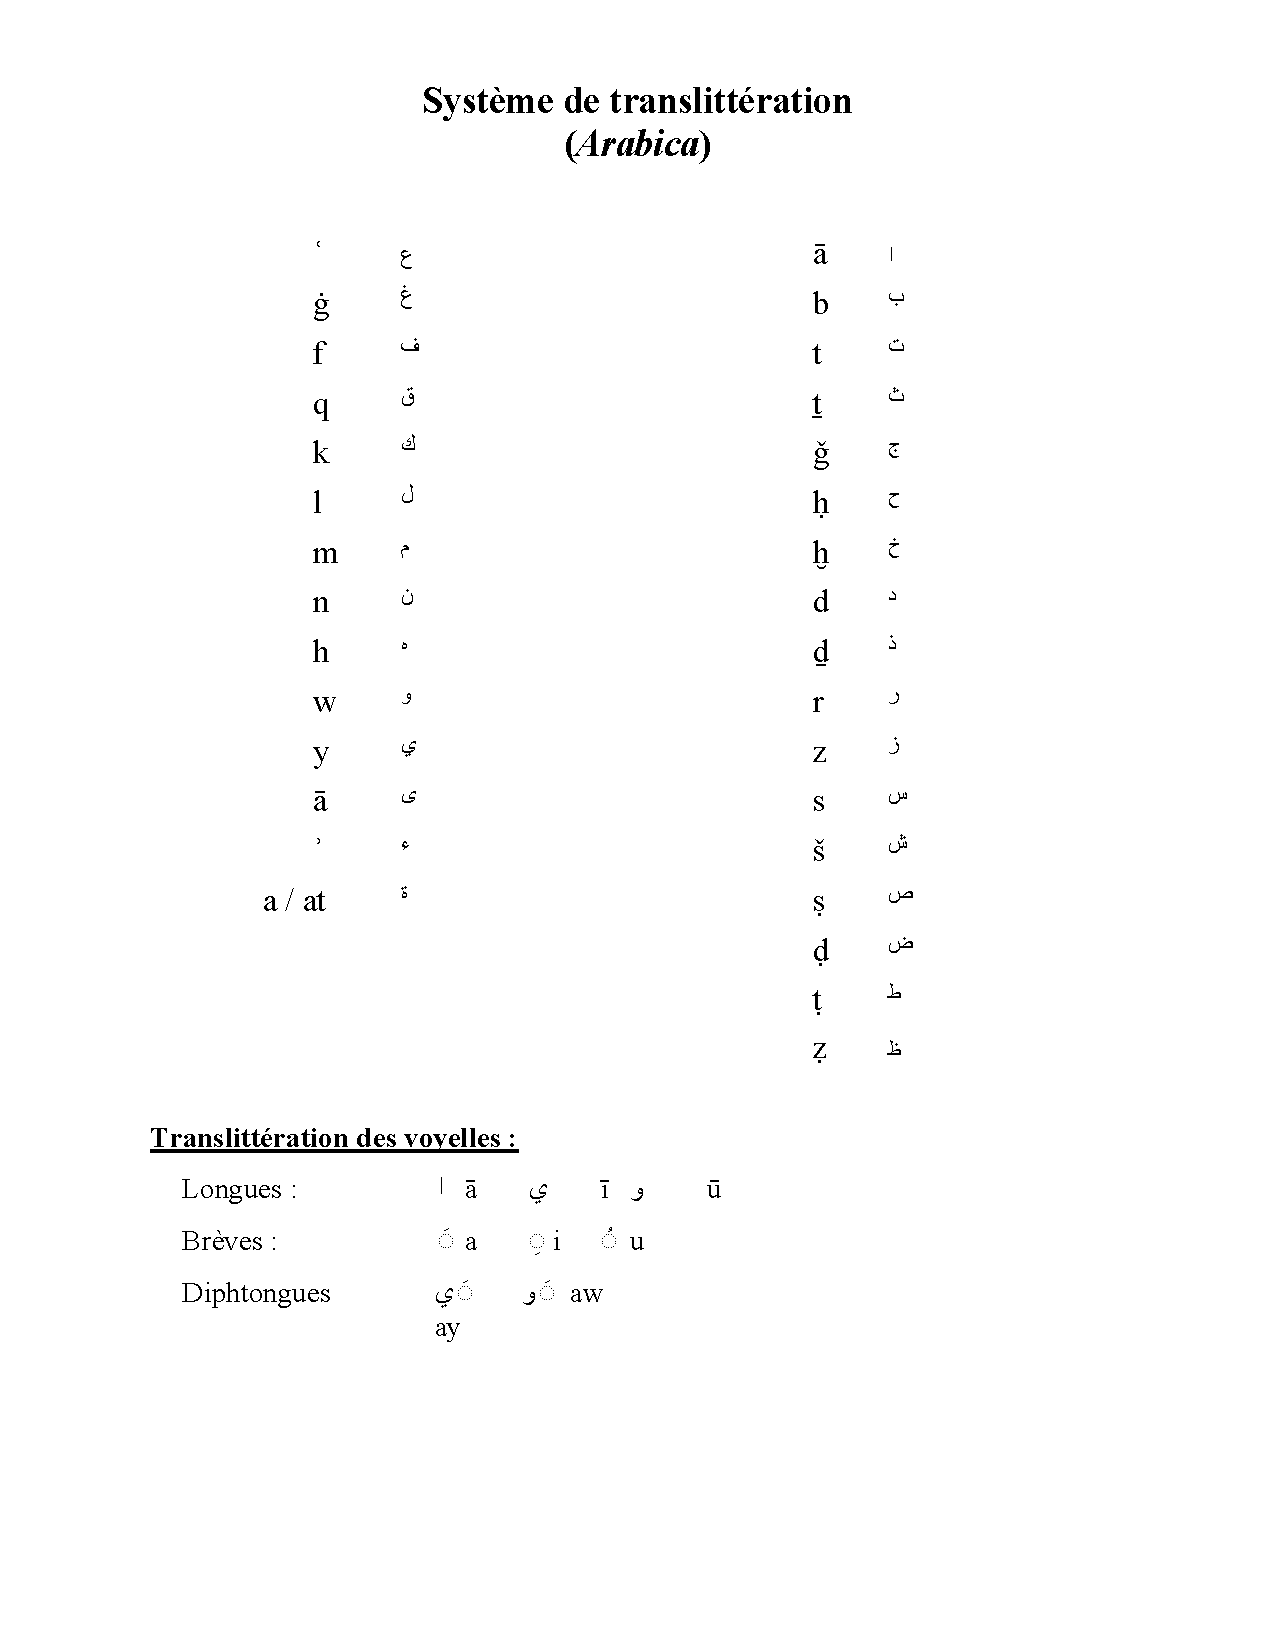
\includepdf{transli.pdf}












\newpage
\pagenumbering{roman}
\setcounter{page}{4}

\chapter*{Notes préliminaires}
\addcontentsline{toc}{chapter}{Notes préliminaires}

\thispagestyle{empty}
Depuis quelques années le monde de l'édition des textes et documents manuscrits (antiques, médiévaux et modernes) vit un basculement vers d'autres horizons. L'introduction progressive de l'outil informatique a changé complètement les méthodes, les pratiques \footnote { Voir par exemple : le site de Stefan Hagel, développeur d'un logiciel pour l'édition critique des textes   \url{ https://cte.oeaw.ac.at/} 

Ou cet outil pour la collation des manuscrits \url{https://cental.uclouvain.be/chrysocollate/} Ou ce nouveau logiciel de visualisation et modélisation VCEditor, conçu par  \textit{Schoenberg Institute for Manuscript Studies} de l'université de  Pennsylvania et autres universités  \url{https://viscoll.org/} } et exigences de l'édition des textes et documents. De plus en plus, on parle ces dernières années d'une édition électronique et d'édition sur support électronique ou d'édition hybride \footnote{ voir par exemple l'édition électronique du chef-d'œuvre de la littérature française moderne : Madame Bovary de Gustave Flaubert \url{ https://www.bovary.fr/ } dernière consultation le 08 août 2022.}  
\paragraph{}

Pour accompagner ( très modestement) ce changement et cette révolution numérique, nous avons  rédigé les  deux parties de ce  travail ( l'édition, la présentation \& le commentaire)  avec  le langage d'édition et système de composition des documents \LaTeX   .

Les vertus de ce langage  de rédaction  professionnelle  sont innombrables. En plus  d'une haute et irréprochable qualité typographique, il permet, pour l'éditeur scientifique, de générer des textes très soignés, logiquement organisés et surtout de gérer efficacement son apparat critique, ses paragraphes, indexes, glossaires, \textit{stemma codicum} ,...etc. En un seul mot, d'avoir en main ou presque les éléments et étapes de son édition. \footnote { L'auteur de ce mémoire  a volontairement appris  ce langage spécialement pour rédiger ce travail. il n'avait eu aucun acquis préalable. Notre ambition de départ était d'éditer avec un  \textit{package} spécial de Latex conçu pour l'édition des textes:\textit{ ekdosis}. Pour diverses raisons nous avons dû renoncer à ce choix. Le grand avantage de ce \textit{package }est la  conversion vers le format TEI xml

Pour plus de détails sur les avantages de \textit{ ekdosis}  voir le blog personnel de Robert Alessi, le développeur du package \url{http://www.robertalessi.net/.}  Dernière consultation le 08 Août 2022. Attention, à cause des bugs le blog n'est pas souvent accessible. 

Ou  ce petit billet de présentation générale et rapide du package sur le blog de L’ÉquIHSAM (Équipe Internationale d’Histoire des Sciences Antiques et Médiévales) (\url{https://equihsam.hypotheses.org/outils-numeriques/ekdosis.} 
Dernière consultation le 08 Août 2022.

Je tiens à remercier vivement Madame Emmanuelle Kuhry  post doctorante à l’IRHT (l'Institut National de l'Histoire des Textes) de m'avoir indiquer l'existence de ce package d'édition multilingue des textes.}  

\newpage 
\thispagestyle{empty}

 Le mode de fonctionnement de \LaTeX   est différent des autres outils et logiciels de rédaction sur un point capital. Contrairement aux logiciels de rédaction ordinaires qui se basent sur le principe de WYSIWYG ( What You See Is What You Get ), \LaTeX  fonctionne selon le principe de WYMIWYG  ( What You Mean Is What You Get ).   Entre voir et donner sens il y a, sans aucun doute,  tout un écart. 


TeX est le début d'un terme grec qui veut dire : art, science . Le système \LaTeX   a été créé dans les années 1980  par le mathématicien, l'informaticien américain et  professeur émérite à l'université de Stanford Donald Knuth   \footnote{  \url { https://www-cs-faculty.stanford.edu/~knuth/index.html} dernière consultation le 08  août 2022. }. Le trait de génie du professeur  Knuth est de confier \LaTeX \TeX à l'American Mathematical Society et d'en faire un logiciel libre.  \LaTeX est aujourd'hui la référence pour la rédaction  professionnelle des documents dans les centaines de revues scientifiques dans le monde. Il existe en version bureautique ( \TeX Maker, \TeX studio...etc)  
et ligne (overleaf \aiOverleaf ) \footnote {\url{https://www.overleaf.com/project} La version de \LaTeX en ligne \aiOverleaf 
offre plusieurs avantage: le travail collaboratif, une compilation plus rapide, une documentation riche et à jour, dès exemples de travaux,  enregistrement en ligne instantané et automatique, possibilité de téléchargement ou de partage..etc

Le site de référence pour l'actualité, mise à jour et nouveauté \LaTeX  est : The Comprehensive TEX Archive Network \url{ https://www.ctan.org/}
}   

L'écriture de droit à gauche a été introduite plus tard, elle exige souvent le passage  par un compilateur-éditeur spécialisé. Dans notre  cas (la langue arabe ) nous avons utilisé l'éditeur  \XeLaTeX. Il existe aussi le compilateur Lua\LaTeX .  

\paragraph{
}La rédaction d'un travail  dans deux langues différente n'est pas du tout facile, il nécessite une attention particulière à beaucoup d'aspects dans chaque langue. L'auteur du mémoire a fourni un maximum d'efforts pour rendre un travail correcte sur tous les plans. Nous sommes conscients que l'explication de certains dimensions de notre travail tel que: les mécanismes de transmission de savoir en Islam médiéval ou sur les variantes de lecture  est en soi un/des projet (s). Nous avons essayé de donner autant que possible une bibliographie permettant au lecteur d'élargir certains points ou d'aller plus loin que nous. 









\chapter*{Introduction générale}
\addcontentsline{toc}{chapter}{Introduction générale}
\pagenumbering{arabic}
\setcounter{page}{1}


\textgoth{L}e texte  édité que nous proposons de présenter  et d’en commenter une partie est  \textit{Kitāb al-ḥuǧǧa f\=i al-qirāʾāt al-sabʿa}. Il est  une œuvre fondamentale de la littérature classique sur le Coran et, plus précisément, sur les Variantes de lecture coraniques dites ( \textit{qirāʾāt} ). Cette oeuvre a été rédigé par le grand grammairien du IV/X siècle: Abū ʿAlī al-Fārisī. Les variantes de lecture  sont considérées comme une discipline qui s’intéresse aux différentes façons de réciter/lire le texte coranique. Elle est née, sans vraiment porter le nom ( \textit{qirāʾāt} ), celui-ci s’imposa  tardivement vers le troisième et le quatrième siècle de l’ère musulmane.  

L'importance de l'ouvrage  est de présenter une idée sur les débuts de la reconnaissance  effective des Variantes de lecture et particulièrement, le système dit de sept lecture ( voire la suite du  travail). Ce dernier  consiste  à adopter des lectures  et de rejeter des autres pour des raisons diverses: non adéquation avec la langue arabe ou les voies de transmission de ces lectures ne sont pas fiables...etc. \footnote{ En plus de ce système de sept lecture, il existe aussi d'autres systèmes : les dix lectures, les quatorze lectures ...etc}
\paragraph{}

 Abū ʿAlī al-Fāris\=i se situe  dans cette œuvre à  la jonction de deux disciplines relativement autonomes. La première discipline   est la grammaire et la philologie arabe ( \textit{al-naḥw wa al-luġa} ) . La deuxième discipline est  consacrée et promue par les lettrés musulmans comme domaine d’étude : les Variantes de lecture coraniques \textit{qirāʾāt} ( voir  la définition ci-après)\footnote { Cette même dichotomie est  reprise dans les travaux et études universitaires et scientifiques. L'ambition de ce travail est de proposer de réfléchir sur les Variantes de lecture à partir d'une perspective interdisciplinaire }. Ce qui réunit la grammaire et les variantes de lecture est la langue, ce qui les différencie est aussi et paradoxalement la langue. 
 
Alors que la grammaire  étudie la langue des locuteurs arabes  ( une langue dans son acception générale et étendue)  ou, ce que les grammairiens désignent par   \textit{al-kalām  al-mawḍūʿ } ( la  parole conventionnelle et positive ), les variantes de lectures est une discipline qui  étudie  exclusivement la langue  du Coran  \textit{al-kalām al-muḥa}̄ (  la parole   révélée  ).Il faut noter et préciser que le Coran est  pour les musulmans  la parole de Dieu \textit{ipsissima verba}, révélée en langue arabe. 

\paragraph{}
En  utilisant le terme  discipline, nous voulons surtout insinuer le fait qu’au début les deux disciplines ( la grammaire et les variantes de lectures) étaient indissociables l'un de l'autre. Par la suite, chaque  discipline  a constitué son propre appareil conceptuel et terminologique,  ses lettrés, ses traités et ses compilations ( \textit{muṣanafāt} ). Ceci est bien visible à partir de la fin du III/VIII ème siècle . Régis Blachère remarque que  « Les premières traces d'une réflexion grammaticale apparaissent dans le courant de VIIIème siècle principalement dans le milieu  des lecteurs  ( \textit{qurā}ʾ), spécialistes du texte coranique, dont ils s'emploient à fixer le texte  en vue de sa récitation. » \footnote{ Blachère Régis, 1952-1966.\textit{Histoire de la littérature arabe}, vol. I. Paris : Libraire Amérique et d'orient Adrien-Maisonneuve, p. 108-110. Cité par Guillaume Jean Patrick  dans:  « L'hypothèse grecque et le débat sur les origines de la tradition grammaticale arabe», in : \textit{Histoire Épistémologie Langage}, 43-1, 2021. p. 62.  

Jean Patrick Guillaume souligne aussi très brièvement dans le même contexte les massorètes de la tradition hébraïque et des \textit{maqreyyane} de la tradition syriaque.}  

Dans le même sens des propos de Balchère, nous pouvons citer trois exemples  témoignant d'une relation étroite entre réflexion sur la langue et la réflexion sur le Coran et ses variantes de lecture


\hspace*{1cm} \ding{172} Dès le début le Coran constitue un sujet de réflexion grammaticale . Par exemple,  Dans le premier traité de grammaire qui nous est parvenu ( Kitāb de Sībawayh (m. ? 176) ) le Coran et la poésie représentent la matière essentielle de ce traité.   \footnote {ʿUḍayma ʿAbd al- Ḫāliq, \underline {Fahāris  Kitāb de Sībawayh}, ?, ?, 1985, pp. 720-761.

Nous soulignons que l'auteur de l'index adopte la seule Variante de lecture de Ḥafs, la plus dominante aujourd'hui dans le monde musulman . Ceci nous prive de poursuivre les autres variantes de lecture  dans le  Kitāb. } 

\hspace*{1cm} \ding{173} Deux parmi les sept lecteurs sont aussi des illustres grammairiens:    abū ʿAmr b. al- ʿAlāʾ (m.154/770) et al-Kisāʾī (m.189/804). Si nousn consultons les premiers  traités de \textit{ Ṭabaqāt }  (littéralement: «classes )\footnote{un genre littéraire spécialisé dans la recension et le classement des auteurs et savants de chaque discipline.  } consacrés aux grammairiens et lecteurs du Coran   «\textit{( « qurāʾ)}  nous rendons compte que les uns et les autres ne font qu'un \footnote{ A titre d'exemple, l'un des plus anciens ouvrages biographiques des grammairiens et philologues  de	al-Zabīdī abū Bakr (m.379/989) 

\underline {Ṭabaqāt al-naḥwiyīn wa al-luġawiwīn}, (éd) Abu al-Faḏl Ibrāhim,  le Caire, Dār al-maʿārif , 1984.} 
 
  

\hspace*{1cm}\ding{174} A partir de la fin du II et le début IIIème siècle, des grammairiens et philologues ont rédigés  des ouvrages entièrement consacrés à l'étude du Coran. On peut citer à titre d'exemple :  


    \hspace*{2cm} \ding{43} \textit{maʿānī al-qurʾān}  de al-Far\=aʾ (m. 207/822)\footnote {Yaḥyā al-Farr\=aʾ,\underline {maʿānī al-qurʾān}, (éd) ʿAlī al-Nadǧār et al,  le Caire, Dār al-Kutub al-Miṣriyya, 1955.}

     \hspace*{2cm} \ding{43} \textit{maʿānī al-qurʾān}  de al-ʾAḫfaš al-Awsaṭ (m. 215/830)\footnote { Voir la présentation de l'auteur et l'œuvre dans l'introduction de l'éditrice:   Abū al-Ḥassan  Saʿīd b. Masʿada   dit (al-ʾAḫfaš al-Awsaṭ), \underline{maʿānī al-qurʾān}, (éd) Hudā Qarāʿa, maktabat al-ḫānǧī, le Caire, 1990.} 

\hspace*{2cm} \ding{43} \textit{maʿānī al-qurʾān wa muškil iʿrābih} de Quṭrub (m. après 214/229) \footnote {Ce livre a une histoire particulière. Il a été toujours compté comme perdu. Très récemment une grande partie de l'oeuvre  a été retrouvée dans une école religieuse \textit{Z\=awiya} au sud de l'Algérie ( ville de Biskra). Il a été édité et publié en 2021 

Quṭrub  Abū  ʿAlī, 
 \underline{maʿānī al-qurʾān wa muškil iʿrābih} (éd) Moḥamad Laqrīz, Riyad, Dār al-Rušd, 2021
} 
\paragraph{}
Dans les études académiques modernes, l'intérêt porté aux variantes de lecture  dans l'histoire du texte coranique en particulier  ou l'histoire de la langue arabe  d'une manière générale revient essentiellement aux linguistes et philologues allemands. En effet, durant la fin du XIXème siècle, et tout le XXème siècle plusieurs travaux historiques \footnote {comme le grand classique des études coraniques en Occident aujourd'hui: \textit{l'histoire du Coran} de Theodor Nöldeke.  Écrit durant la deuxième moitié du XIXème siècle et traduit un siècle et demi plus tard de l'allemand vers l'arabe en 2004 grâce au soutien de la fondation  Konrad-Adenauer-Stiftung (KAS) sous le titre : \textit{Tārīḫ al-quraʾān }.  Theodor Nöldeke,\underline {Tārīḫ al-quraʾān}, revu par Friedrich Schwally, (trad de l’allemand par Géorges Tāmer et al), Beirut, Konrad-Adenauer-Stiftung , 1er éd, 2004.

Et très récemment vers la langue anglaise.
Theodor Nöldeke, \textit{the history of the Qurān}, edited and translated by Wolfgang H. Behn, Leiden, Brill, 2013

Toutefois, il faut souligner aussi que la question de la paternité de l'ouvrage  (\textit{authorship}) reste quand même flou. Un ouvrage rédigé et révisé par quatre auteurs ( tel que figure dans le titre de la traduction anglaise)   Theodor Nöldeke (m.1930) Friedrich Schwally (m.1919) , Gotthelf Bergsträßer (m.1933),Otto Pretzl (m.1941) reflète sans aucun doute l'esprit de travail collectif mais, pour le chercheur ou lecteur cela reste moins clair. } 
ou d'édition des traités des variantes de lecture ont été réalisés. \footnote{ Par exemple le livre des sept lecture canonique :
\underline{ kitāb al-taysīr fī al-qirāʾāt al-sabʿ}a de Al-Dānī Abū  ʿAmr (m.444/1053)  édité et publié par Otto Pretzel (m.1941).

Ou encore le livre des lectures non canoniques : \underline{muḫtasar šaw\=aḏ al-qirāʾāt} de Ibn Ḫālawīh (m. 370/980) édité et publié par Gotthelf Bergsträßer (m.1933) }





Les approches et tendances actuelles de recherche sur Coran et les Variantes de lecture sont très diverses: Il  existe les approches historiques, les approches philologiques mais également les approches littéraires et l'étude des manuscrits coraniques. Durant les vingt  dernières années plusieurs   projets de recherche ont vu le jour \footnote{ Comme le projet allemand  Corpus coranicum,  créé en 2007 par la Berlin-Brandenburgische Akademie der Wissenschaften pour une durée de dix-huit ans, jusqu’en 2024. Voir le site du projet sur  {\url{ https://www.bbaw.de/}  dernière consultation le 8 août 2022} 

Ou encore le projet « Le Coran Européen : l’étude du Texte Sacré de l’Islam à travers la Culture et Religion Européenne 1150-1850 » (EuQu) pour une durée de six ans 2019-2025. \url{https://euqu.eu/} dernière consultation le 8 août 2022. 

Ou la création de chaires revues et chaires spécialisées. A titre d'exemple Histoire du  Coran. Texte et Transmission : 
\url{ https://www.college-de-france.fr/site/histoire-coran-texte-transmission/Presentation.htm}  } , des colloques internationaux \footnote{ Comme  le dernier colloque qui s'est tenu le 2-3 Juin 2022 à Paris.
Voir la retransmission des interventions sur  \url{https://www.collège-de-france.fr/site/francois-deroche/symposium-2021-2022.htm} dernière consultation le 8 août 2022} et des publications scientifiques encyclopédiques\footnote{Comme: Mohammed Ali Amir-Moezzi et Guillaume Dye (dir), \textit{Le Coran des historiens}, Paris, les Éditions du Cerf, 2019.}.   

Au delà des approches appliquées ou les résultats de recherche attendus, nous avons constaté  que les recherches qui se font sur le variantes de lecture (l'objet de notre étude ) s'articulent autour de  trois axes, certains axes sont plus représentés que d'autres:   

\begin{itemize}
    

 \item 	Les variantes  sont explorées exploré du point de vue de leurs relations avec le squelette consonantique \textit{le rasm} des vieux manuscrits coraniques . Cela veut dire alterner entre d’une part, les vieux témoins manuscrits du \textit{rasm }coranique  et de l’autre part les variantes telles que repérées (ou pas) et reconnues  par la Tradition islamique postérieure. \footnote{ On peut citer surtout les travaux du professeur François Déroche. voir le lien vers le collège de France cité plus haut. }  

 \item   Certains recherches s'intéressent aux voies de transmission des Variantes de lecture  \textit{isanād } et  les critères d’adoption  ou de rejet d’une lecture  appliqués par les savants musulmans à travers les siècles.  \footnote{ On peut citer les deux récentes études de : 

 Shady Hekmat Nasser, \textit{The transmission of the Variant Readings the problème of tawātur and the émergence of shawādhdh}, Leiden-Boston, 2013.

 Chahdi  Hassan, \textit{Le muṣḥaf dans les débuts de l'islam : recherches sur sa constitution et étude comparative de manuscrits coraniques anciens et de traités de qirā'āt, rasm et fawāṣil}, Thèse de doctorat inédite, sous la direction de François Déroche, École pratique des hautes études, Paris, 2016. 
 
 }  

 \item  Les variantes de lectures  font l’objet d’études syntaxiques et lexicales. C’est-à-dire  comment les premiers grammairiens ou lexicographes ont perçu les Variantes d’un point de vue strictement linguistique. Et de voir surtout comment ils ont dirigé par leur théories soit sur le\textit{ rasm}  soit encore sur les modes de récitation du Coran.  

\end{itemize}

Notre projet de mémoire ne s'intéresse pas au \textit{rasm} ni au \textit{isnad} des variantes de lectures. Cela demande des recherches plus profonde. \footnote {Le lecteur qui s'intéresse au \textit{rasm et isna\=ad} peut consulter les travaux  que nous venons de citer ou les traités de \textit{rasm} des érudits musulmans. Le plus connu :  \textit{Al-muqniʿ fī rasm al-muṣḥaf }de Abū ʿAmr al-Dānī et autres } . Notre travail  se focalise principalement sur l'édition,   la grammaire des variantes et  les modalités de la transmission des textes.

Nous  travail est composé de deux grandes parties : la partie édition et la partie présentation et commentaire.  

Il faut d'abord  souligner que les pratiques  de l'édition des textes manuscrits sont très diverses. l'édition  peut être complète ou partielle, universitaire, définitive,  savante,  destiné à un large publique...etc.  Les méthodes appliquées par les éditeurs scientifiques   sont  également très divers, nous avons surtout :   

           \ding{243}     Édition d'un texte + annotation:  l'intérêt et la fonction de l'annotation peuvent être historique et littéraire, philologique ou ( simplement) explicatif.

            \ding{243}   Édition d'un texte + commentaire : soit un commentaire minimal d'un texte soit un commentaire élargi ( historique, intellectuel et doctrinal ,grammatical...etc)    

             \ding{243}   Édition d'un texte + présentation : Pour expliquer les voies de  la transmission, les modalités et agents de la diffusion  et la réception  d'une œuvre selon les époques et les géographies.  

             \ding{243}   Édition d'un texte + traduction : Pour permettre  un accès à un public  non spécialisé.  

             \ding{243}	l'établissement des index analytiques ou des glossaires fait partie aussi des méthodes de l'édition. Cela  permet de  donner un accès non linéaire à une œuvre. 



Notre  édition est divisé en plusieurs chapitres. Nous avons commencer par le titre donné à  l'œuvre (\textit{kitāb al-ḥuǧǧa f\=i al-qirāʾāt al-sabʿa}).   Ensuite, l'introduction de l'auteur et la sourate 30. 

La richesse de l'un des  manuscrits de cette étude  ( [M] ) dépasse le cadre du contenu intellectuel. Il contient des éléments importants pour l'histoire de  \textit{Kitāb al-ḥuǧǧa}.  (  notes de  possession, certificats de lecture-audition et licence de transmission)  Nous avons estimé que l'édition des ces élément péri-textuels permet de jeter un nouveau regard  sur   \textit{Kitāb al-ḥuǧǧa}. La dernière partie de l'édition est consacrée à l'édition des éléments péri-textuels.      


Quant à la deuxième grande  partie de ce travail   ( la présentation et commentaire)  
elle contient cinq partie: 1) une brève présentation définitionnelle et historiques des Variantes de lecture coranique.  2) une introduction à l'édition contenant une présentation de l'auteur et son œuvre, une présentation des manuscrits de   ainsi que  principes de l'édition     3) un commentaire et analyse du titre, le prologue et  de quelques variantes choisies de la sourate édité  4)  commentaire des éléments péri-textuels édités.   
 
  


%%%%%%%%%%%%%%%%%%introduction générale


%%%%%%%%%%%%%%%%% la première partie I

\chapter{Les variantes de lecture coraniques \textit{qirāʾāt} : un  bref aperçu définitionnel et historique}


 
\textgoth{A}vant d'aborder et de présenter les différentes aspects de notre sujet de recherche, il est nécessaire de  donner une  courte esquisse du sujet de notre recherche. Autrement dit, donner un aperçu global sur les  principaux termes qui seront mobilisés au cours de ce mémoire. variantes de lecture du point de vue  définitionnel et historique. En premier temps, le sens recouvré par le terme \textit{qirāʾāt} dans la langue arabe. En deuxième temps, nous examinons le concept  qui découle du terme \textit{qirāʾāt} et comment les érudits musulmans ont défini les variantes de lecture coraniques? Finalement, nous exposons brièvement les deux principales thèses sur l'émergence des variantes de lecture coraniques et quelques notes sur les variantes de lecture d'un point de vue théologique. 

 
\section{A quoi renvoie le terme \textit{qirāʾāt} ? }



\paragraph{}
L’expression technique \textit{al-qirāʾāt al-qurʾāniya} (littéralement : les lectures coraniques) Ou, simplement en forme  abrégée sans détermination,  \textit{qirāʾāt  } désigne les variantes du texte du Coran ; des Variantes entendues dans le sens général du terme.\footnote{ une variante peut être graphique, orthographique, phonétique, syntaxique...etc}. Assigner des limites définitionnelles au terme  et retracer son développement dans la conscience des érudits musulmans des premiers temps de l’Islam est très difficile. Cependant, la consultation des traités spécialisés des \textit{qirāʾāt }  permet de  donner  une double référence au terme.
\paragraph{}
D'une part,  le terme \textit{qirāʾa} ( lecture  )  au singulier sert à désigner les variantes textuelles du Coran  avec une référence directe à un  lecteur du Coran ( \textit{qāriʾ} ) ou à un transmetteur ( \textit{rāwī }) . C'est ainsi qu'il est dit très souvent par exemple:  \textit{qirāʾat} ʿĀṣim, \textit{qiārt}  al-Kisāʾī  (i.e. la(s) variante(s) de lecture tel que rapporté par ʿĀṣim) (la(s) variante(s) de lecture tel que rapporté par  al-Kisāʾī…etc ). 
\paragraph{}
De l'autre part,  le terme dans sa forme plurielle caractérise l'ensemble des traités et compilations portant sur ces même variantes. Par exemple : le livre de \textit{qirāʾāt} de Ibn al-Ǧazarī, le livre de \textit{qirāʾāt} de ʾAbū ʿAmr al-Dānī…etc. La forme plurielle définit aussi  la discipline elle même dite:\textit{ʿilm  al-qirāʾāt} (littéralement « science des lectures [coranique] ) d'où la traduction vers le français par  Variante (s) de lecture et vers l'anglais par \textit{Variant Reading(s)}. Que ce soit en langue arabe ou dans les traductions le terme variantes de lecture  dénote la multiplicité et la variance.  Le terme \textit{qirāʾāt}  dans sa forme plurielle ou au singulier n'est pas coranique. Toutefois, la forme verbale \textit{qaraʾ} revient dans le texte coranique dans plusieurs environs (70 occurrences)  avec  des sens et nuances très divers selon le contexte d'emploi. 

\paragraph{}
Enfin, il n'est pas aussi sans intérêt de rappeler ici  que  l'origine même du terme  qui sert  à designer l'ensemble du texte sacré des musulmans: le Coran ou  \textit{qurʾān } en langue arabe pose aussi un problème dans la communauté des chercheurs. Certains adhèrent à l'avis musulman selon lequel le terme est issu de l'arabe coranique. ( des dizaines de fois dans le Coran avec un sens peu stable et varié). D'autres chercheurs estiment que \textit{qurʾān } est étymologiquement non arabe. le mot  serait l'équivalant de \textit{ḳeryānā} (lecture des Écritures, leçon )    de la liturgie chrétienne. \footnote {Pour plus de détail voir: Welch, A.T., Paret, R et al, « al-Ḳurʾān » \textit{ EI2}, Leiden, Brill, (en ligne.)  }

Quant à notre terme \textit{qirāʾāt} avec ses dérivés, il reste peu précis.  Dans le texte édité ci-joint,  \textit{qaraʾ}   ne recouvre sens, indication  ou référence à quelque chose  l'écrit. \textit{qirāʾāt} serait peut être le synonyme de : prononcer selon  un certains idiomes sociolinguistiques,  ou selon la variante locale ou régionale...etc   

 \newpage
\section{ \textit{Qirāʾāt} : genèse, évolution et fixation postérieur d’un concept  }


Au-delà du sens terminologique et linguistique, la définition des\textit{ qirāʾāt} comme concept et terme spécialisé est également intéressant à montrer. Celà nous permet d’esquisser les représentations du concept à travers les siècles et de montrer comment les variantes de lectures ont été érigées et promues en discipline autonome.  Pour définir le concept de Variantes 
de lecture, il est plus que nécessaire de revenir aux définitions proposées par les premiers érudits musulmans. 

\paragraph{}
L'ouvrage de référence  en la matière \textit{Kitāb al-sabʿa} ( le livre des sept lectures )  rédigé par Ibn Muǧāhid  (m.324/936) \footnote{Aḥmad b. Mūsā b. al-ʿAbbās Abū Bakr al-Tamīmī  est un savant né à Baghdad 245/859.

Voir: Robson, J, « Ibn Mud̲j̲āhid », \textit{ EI2}, Leiden, Brill, (en ligne.) }   
ne contient pas une définition aboutie des Variantes de lecture coranique. La longue  introduction de  l'auteur  (56 pages) ou la présentation doctrinale de l'éditeur du livre  Šawq\=i Ḍayf (40 pages)  ne permettent pas d'avoir  une définition claire et bien nuancée des Variantes de lecture car, l'une et l'autre sont trop descriptives .  Dans son introduction,  Ibn Muǧāhid énumère les sept lecteurs et leurs généalogies (\textit{nasab}) pour passer aux chaînes  de transmission ( \textit{asānīd })   de chaque lecteur. 
\footnote{Ibn Muǧāhid Musā, \underline {kitāb al-sabʿa,} , (éd) Ḍayf Šawqī, Le Caire, dār al-maʿārif, 1972.}  

\paragraph{}
Toutefois, ce qui se prête  à une définition  des variantes de lecture dans l'ouvrage d' Ibn Muǧāhid est les critères de choix  adoptés pour restreindre les lectures à sept.  Voici tout d'abord ce  dit Ibn Muǧāhid dans l'introduction  « Les transmetteurs du Coran ( \textit{ḥamalat al-qurʾān}) ne reproduisent pas tous de la même façon les données coraniques, chacun d'eux occupe une position dans la reproduction orale, qui lui est propre. Je me propose d'indiquer [dans cet ouvrage]  la position qu'ils ont occupée et de désigner ceux d'entre eux qui furent des maîtres, enfin, les système de reproduction qui sont actuellement en cours au Hédjaz, dans l'Iraq et en Syrie [...] parmi ces transmetteurs, il ya: 
\begin{enumerate}

    \item  Celui qui respecte la grammaire ( \textit{muʿrib})\footnote{participe actif tiré de \textit{iʿr\=ab} } et qui connaît toutes les ressources de l' 
    (\textit{iʿr\=ab}) et de variantes de reproduction coraniques ( \textit{qirā ʾāt} ) qui est Coran des Variantes locales de reproduction ( \textit{luġāt}) et des significations assignées au discours ainsi que les défauts inhérents à ces reproductions...» 
    \item Il y a également celui qui respecte la grammaire et ne commet pas d'incorrections ( \textit {lā yalḥan)} mais qui ne possède, hormis cela,  aucune autre connaissance...

    \item Il y aussi le cas de celui qui reproduit (machinalement) les réalisations qu'il a entendues de son informateur et qui ne peut faire autre chose que de reproduire ce qu'il a appris. Il ne connaît ni \textit{iʿr\=ab} ni rien d'autres. Il s'agit là du \textit{ḥāfiḏ } ( qui se borne à mémoriser un texte)...»

    \item Il y a enfin celui qui applique l'\textit{iʿr\=ab} dans sa reproduction et connait les significations  qui s'y rattachent ainsi que les variété de substrat mais qui n'a, en revanche, aucune connaissance des variantes de reproductions coraniques et des divergences qui existent entre les transmetteurs ainsi que les traditions y afférentes....\footnote{ Ibn Muǧāhid Musā, \underline {kitāb al-sabʿa,} , (éd) Ḍayf Šawqī, \textit{op.cit}, pp. 45-46. 
    
    Pour la traduction des passages cités voir: Hadj-Salah Abderrahman, \textit{linguistique arabe et linguistique générale essai de méthodologie et d'épistémologie de 'ilm al-'arabiyya}, Alger, Publications de l'Académie algérienne de la langue arabe, 2011. Vol. I, pp.117-118.}
\end{enumerate} 


La  réforme et l'innovation de   Ibn Muǧāhid des Variantes de lecture ( au début du IV) et les critères choisis pour restreindre et limiter ces lectures  au nombre sept \footnote{Dans le langage des Variantes de lecture  Ibn Muǧāhid est désigné par:\textit{ musabiʿ al-qirāʾāt} ( celui qui a limité les lectures coraniques à sept } ont, d'une part  orienté toute conception ultérieure des variantes de lecture et de l'autre part, l'apparition de système de lectures non canoniques (\textit{šāḏa} ). En bref, jusqu'à nos jours les variantes de lectures dans la Tradition musulmanes sont soit: 

\ding{100} Des lectures canoniques dites ( \textit{qirāʾāt mutawātara}): il s'agit de lectures reconnues, attestées par les théologiens musulmans. Ces lectures  sont globalement ceux de  Ibn Muǧāhid  

\ding{100} soit encore des lectures non-canoniques dites ( \textit{qirāʾāt šāḏa}): Il s'agit globalement  de lectures existantes et attestées mais non-reconnues par la théologie musulmane   

 \textit{Kitāb al-sabʿa} constitue jusqu'à aujourd'hui la pierre angulaire de la discipline des variantes de lecture. Il est le début d’une longue histoire, celle de la reconnaissance effective et  de la prise en compte des Variantes de lectures comme réalité textuelle  et surtout comme une donnée coranique. 
 L'empreinte de son auteur Ibn Muǧāhid est  bien visible dans les ouvrages qui sont venus après lui (après le IV siècle). Désormais, les théologiens musulmans prêtent attention à définir et le Coran et les variantes de lecture.   Citons deux brèves définitions  dans deux époques différentes. 
 
 Pour al-Zarkašī (m.745/1344)  le Coran et les Variantes de lecture sont deux réalités distinctes ( \textit{ḥaqīqatāni muḫ̬talifatāni} ).\footnote{al-Zarkuši Muḥamed,  \underline {al-burhān fi ʿulūm al-qurʾān} , (éd)  abu al-Faḍl Ibrāhim, le Caire, maktabat D̄ār al-turāṯ, le Caire,  p. 318. } En effet, dans son ouvrage consacré  au texte coranique \textit{al-burhān fi ʿulūm al-qurʾān}, il définit  les variantes de lecture ainsi: 

« \textit{al-qirāʾāt hiya iḫtilāf alfāḍ al-waḫy al-maḍkūr fi katabat al-ḥurūf wa kayfiyātihā min taḫfīf wa taṯqīl wa ġayrihā.} »

« Les Variantes de lecture sont une divergence dans les termes de la révélation [coranique] [tel que] mentionné par les scribes des lettres [du Coran] ou leurs divergences, allégées ou alourdies  soient-elles  [ de ces lettres] ou autre »


L’un des grands  érudits des variantes de lecture Ibn al-Ǧazar\=i  (m. 833/1429) a , quant à lui, une autre conception des variantes de lecture. voici comment les variantes de lecture sont définies
\textit{ʿilm bi-kayfiyāti ʾadāi kalimāti al-qurʾān wa iḫtilāfih\=a bi-ʿazwi al-nāqilati }. » 

 « une connaissance des  manières de réciter  les mots du Coran et les   divergences dans la récitation  selon les chaînes de transmission. »

















\section{	L’émergence des variantes de lecture entre :\textit{ rasm } et \textit{riwāya}}


L’émergence des Variantes de lecture et leurs reconnaissance tardive par la tradition musulmane comme  une partie intégrante du texte coranique est un fait historique de grand importance qui a attiré l’attention des chercheurs depuis fort longtemps. La question qui s’est posée alors, et se pose  encore aujourd’hui : comment et dans quel contexte historique  les Variantes de lecture du texte coranique ont vu le jour ?  Comment le texte coranique, supposé être un, devient ou presque multiple ?  Que peut nous renseigner cette multiplicité de Variantes de lecture sur les voies de transmission du Coran ? 

\paragraph{}
D’une manière générale, il existe deux principales thèses opposées sur le contexte de l’émergence des Variantes de lecture. La première et la  plus ancienne thèse est celle de la tradition musulmane, elle embrasse les trois aspects le dogmatique, l’historique, le philologique et quelques fois le mythique.  La deuxième thèse  remonte au dix-neuvième siècle, elle a vu le jour dans le sillage de l'intérêt occidental pour le texte sacré des musulmans.  
\paragraph{}
Pour la Tradition musulmane, la multiplicité des Variantes textuelles dans le Coran s’explique essentiellement par le processus par lequel ces mêmes Variantes ont dû passé : \textit{la riwāya} (la transmission orale ) d’une génération à une autre. Rappelons dans ce sens qu’a l’origine le Coran n’est pas un texte écrit mais plutôt il s’agit des propos de style oral. Les canaux de la diffusion de ces propos et enseignements  fut principalement l’oralité. L’existence ou l’exercice d’une culture lettrée écrite  dans le début de l'Islam est timidement évoqué par les sources scripturaires musulmanes postérieurs ( I et IIème siècle H).  

En effet, avant le développement de l’écrit dans les siècles qui ont suivi la mort  du prophète Muḥammad, La \textit{riwāya} fut le mode de transmission dominant et privilégiée en Arabie pré-islamique ou durant les débuts de la mission du prophète de  l’Islam. La transmission par voie de récitation orale constitue la norme de diffusion des propos quel que soient la nature.  Cela vaut aussi bien pour la poésie pré-islamique et islamique, la collection et la canonisation du  ḥadit̠h  et les autres aspects de la vie sociale et culturelle en Arabie.  L’universitaire et islamologue suisse Grégor Schoeler va plus loin en affirmant fortement que : 

\paragraph{}
« il est incontestable que la poésie archaïque était destinée à l’origine à être récitée et diffusée oralement ; il en allait de même pour la généalogie (\textit{nasab}), les proverbes (\textit{amtha}l) et les récits légendaires et historico-biographiques tribaux- ce que l’on nomme « Journées des Arabes » (\textit{ayyam al-ʿarab}) et « récits » (\textit{akhbar}). L’acte de récitation tenait en même temps lieu de publication et de transmission : pour la poésie, la publication obéissait à donc à un processus absolument différent de celui des contrats. […] après la mort du maitre, la récitation et la diffusion devenaient exclusivement la tâche du transmetteur.»\footnote{Schoeler Grégor,\textit{écrire et transmettre dans les débuts de l'islam}, Paris,PUF, 2002.p.19.
}

  Dans cet environnement et contexte historique les Variantes de lectures  du Coran ont vu le jour. Leurs transmission et diffusion ne constitue pas une exception à cette règle de l’oralité.  Des extraits du texte coraniques  (  \textit{sourate-s} ) au même titre que des recueils de poésie ont été ainsi mémorisés et retenus par les compagnons du prophète et ceux qui l'ont suivi. 
  
  Pour donner un exemple illustratif de  ce contexte  historique de l'émergence des variantes de lecture. L’un des sept lecteurs ( \textit{qurāʾ} )  est  à la fois un transmetteur de la poésie et du Coran. En effet,ʿAbū ʿAmr b. al-ʿalāʾ  (m. 154/770) est l’un des transmetteurs ( \textit{ruwāt} )  de recueils poétiques  du poète omeyyade D̠ī al-R-rumma   (m. vers 117/735-6).\footnote{Pour des informations sur le recueil poétique ( Diwān ) de  D̠ī al-R-rumma     voir la première édition de l’orientaliste britannique C.H.H .Macartney :  Ġaylān b. ʿUqba al-ʿAdawī, \textit{the Diwān of G̲h̲ailân ibn ʿUqbah known as Dhû Rrumma}, (éd), C.H.H .Macartney, Cambridge, 1919. 

Voir également l’excellente introduction de la nouvelle édition de  :  Ṣalāh ʿAbd al-Quddus, particulièrement les pages suivante   
Ġaylān b. ʿUqba al-ʿAdawī, \underline{Dīwān Ḏī al-Rrumma}, (éd) Ab\=u Ṣalih ʿAbd al-Qudus, Beyrouth, muʾasasat al-risāla, 1993, pp. 20-34. }   

\paragraph{}
À  partir de la deuxième moitié  XIXème siècle et dans des divers contextes historiques, intellectuels et politiques une  deuxième thèse concourante et, à certains égard, alternative a vu le jour en Occident. Sous l’impulsion et sur fond  des  découvertes scientifiques majeurs de la deuxième moitié du XVIII ( particulièrement le déchiffrement de l’Hiéroglyphes par  l’égyptologue français Jean François Champollion et le début de la promotion des études du Sanskrit par le philologue britannique William Jones…etc),  l’intérêt pour l'étude des  autres civilisations et cultures  s’est intensifié.\footnote{ Le petit essai  de Markus Messling,\textit{ Les hiéroglyphes de Champollion philologie et conquête du monde}, Grenoble, Ellug,2015. permet de jeter un nouveau lumière historique et de réfléchir aux enjeux historiques, stratégiques et nationaux des grands découvertes du XVIII et XIXème siècle }  
 Dans ce contexte, un ouvrage majeur  sur le Coran voit le jour en Allemagne vers 1860: \textit{l'histoire du Coran} de Theodor Nöldeke ( voir l'introduction). En se basant sur l'étude  des données historiques fournies par la Tradition musulmane Nöldeke souligne le rôle de l'écriture des premiers exemplaires coraniques dans l'émergence et la multiplicité des Variantes de lecture.  
 On sait que les premiers\textit{ masāḥif} ( exemplaires du texte coranique )  étaient dénués de toute signe diacritique ( \textit{iʿǧām} )  et de vocalisation ( \textit{taškīl }). L’absence de ces deux outils indispensables à la fixation  d’une seule prononciation aux mots a eu un impact dans l’émergence  des la tradition musulmane selon l'auteur de \textit{la Geschichte des Qorâns}. L'ouvrage de Nöldeke constitue d'une part, la première interrogation historique sérieuse sur le contexte, les étapes de la constitution matérielle et dogmatique du Coran. 
 De l'autre part,  L'ouvrage de Nöldeke  constituera pour longtemps la matrice explicative et le paradigme historique le plus accepté dans les études occidentales sur le texte sacré des musulmans ou  ce qui est désigné aujourd'hui comme les études historico-critiques sur le Coran.   
 
 Par ailleurs, il faut également noter que l'ouvrage s'appuie sur un nombre considérable de récits plus au moins authentiques ou historiques rapportés dans divers recueils et traité de discipline différentes : hadith, ouvrages biographiques... etc 

\paragraph{}
Pour résumer ce qui vient d’être énoncé, nous pouvons dire que les deux thèses se fondent sur des critères différents. La Tradition musulmane se focalise sur les dimensions orales de la transmission des variantes lecture et les canaux oraux de la circulation du texte\textit{riwāya} avec un silence sur les destin des premiers exemplaires coraniques. La deuxième thèse  s’appuie sur des critères  philologiques et données  paléographiques assorties par une confrontation et examen attentif  et critique  des récits musulmans soutient le rôle des premiers exemplaires coraniques dans l'émergence des variantes de lecture.  

l'histoire de la transmission du texte au début de l'Islam et l'émergence des variantes de lectures est en train d'être réexaminer  depuis dizaines d'années. La découverte des nouveaux témoins manuscrits coraniques  très  anciens(Manuscrit de Sanʿāʾ au Yemen par exemple) et les développements scientifiques récents  dans les études codicologiques et paléographiques a rendu  la question des lectures coraniques au centre d'intérêt. François Déroche, paléographe et codicologue  mondialement reconnu soutient la thèse  d’une transmission mixte orale et écrite   « Sans nier l’importance de la transmission orale et le caractère initialement oral du Coran, comme l’indique son nom même (Qur’ān), il est difficile d’en parler sans évoquer l’écrit. D’une part, la distinction entre les deux volets de la transmission du Coran ne peut être absolument rigoureuse : leur histoire est faite d’allers-retours. De l’autre, comme on le verra, l’écrit a largement conditionné l’oral : négativement, si l’on peut dire, parce que le système d’écriture employé initialement pour noter les révélations était trop déficient pour éviter l’apparition de variantes ; positivement, dans la mesure où le squelette consonantique de la version uthmanienne s’est révélé crucial pour imposer cette dernière et servir de critère pour le canon pensé par Ibn Mujāhid.» \footnote{
Déroche François, \textit{Le Coran une histoire plurielle essai sur la formation du texte coranique}, Paris, Seuil, 2019, p. 74.
 }



\newpage

\section{	Le hadith de \textit{sept aḥruf} et le statut théologique des Variantes de lecture}



Comme nous venons d’énoncer, la tradition musulmane mis en avant l'aspect de l’oralité des Variantes  lecture et que les lectures multiples sont dû  aux transmetteurs. Toutefois, il est intéressant de constater qu' aux alentours de la fin du premier et le début du deuxième siècle la question de de la multiplicité des Variantes de lecture prend un ampleur assez  important. En effet,  dans le contexte de la collection des traditions prophétiques orales dites hadith, certains compilations et traités de ḥadith rapportent ce que nous pouvons qualifier  d’une sorte de multiplicité de récitation du Coran qu’aurait été admise au vivant même du prophète. Cette tradition est plus connu par le hadith de sept lettre ( \textit{sabʿ aḥruf} ), elle constitue le socle commun de tout discours sur les Variantes de lecture d'un point de vue dogmatique. Bien plus, elle donnera un statut théologique  et une légitimation des différents manières de réciter le Coran jusqu'à nos jours. Nous examinons ici  deux points, le premier nous voyons comment cette tradition a été rapporté dans les milieux religieux ? en deuxième nous voyons comment la question a été compris dans quelques études  académiques  récentes.     


Le hadith de \textit{sept aḥruf}  a été rapporté  par des recueils de hadith, des compilations de \textit{fiqh}, des traités de \textit{tafsīr} avec des légères variations et des voies de transmission ( \textit{sanad} )  multiples.
\paragraph{}
La plus ancien source qui a rapporté le hadith  le  livre \textit{ al-muwaṭṭaʾ} du fameux traditionniste  :  Mālik b. ʾAnas (m.179).  Plus précisément, dans la section thématique intitulée:  Kitāb al-qurʾān, 
dans la sous-section \textit{bāb} portant le titre suivant : ce qui est dit du Coran \textit{mā ǧāʾ fi al-qurʾān}. Cette dernière regroupe sept hadith(s) relevant des épisodes coraniques ou prophétiques différentes, celui nous concerne dans cette étude apparaît en premier. Voici comment le hadith est rapporté dans cette compilation. 


De Mālik, de b. Šihāb, de ʿUrwa b. al-Zubayr, deʿAbd al-Raḥmān b .ʿAbd al-qāri, a dit : 
 j’ai entenduʿUmar b. al-H̬aṭāb dire : 


J’ai entendu Hišām b. Ḥakim b. Ḥizām  recite la sourate al-Furqān [sourate 25] d’une façon différente de la mienne et de ce que le prophète -que la paix soit sur lui- m’as appris, J’ai failli me précipiter vers lui, mais je lui ai laissé le temps jusqu’à ce qu’il finisse [sous-entend sa prière]. Je l’ai saisi par son manteau et  je l’ai amené vers le prophète -que la paix soit sur lui- et j’ai dit : prophète de Dieu, j’ai entendu celui-là récite la sourate al-furqān différemment de ce que vous m’avez appris. [alors] le prophète a dit laisse-le partir, puis a dit : récite . Il a récité de la mémé façon qu’avant. Le prophète-que la paix soit sur lui- et a dit il a été révélé ainsi. Puis m’a dit : récite et j’ai exécuté, et il a dit : c’est ainsi [cette sourate] c’est révélé, \textbf{ce Coran a été révélé selon sept lettres [ʿalā sabʿi aḥruf]  lisez ce que vous pouvez.}» \footnote{Anas b. Mālik, \underline { al-muwaṭṭaᵓ riwāyat yaḥya b. yaḥya al-Layṯi}, (éd) Publications du haut conseil scientifique, 2ème éd, Vol 1,  Rabat, 2019, p.375.}  
\paragraph{}
 Le \textit{matn }du hadith ( l’information transmise ) ci-dessus retrace ce qui semble être comme un fait divers presque insignifiant de la vie quotidienne. Il y a une mise en narration progressive, emboîtée et dirigée pour la résolution d’un seul problème mais, narrativement parlant, elle n’est ni singulière ni unique dans son genre. Tout au contraire, elle est similaire et très fidèle au langage et terminologie du Ḥadith d’une manière générale.  


     Le \textit{matn} du hadith  ci-dessus retrace ce qui semble être comme un fait divers presque insignifiant de la vie quotidienne. Il y a une mise en narration progressive, emboitée et dirigée pour la résolution d’un seul problème mais, narrativement parlant, elle n’est ni singulière ni unique dans son genre. Tout au contraire, elle est similaire et très fidèle au langage et terminologie du Ḥadith d’une manière générale.  

En revanche, ce qui  mérite  d’être souligner c’est que  le récit-cadre des propos rapportés. Il  s’articule autour de trois protagonistes dont la fonction et la valeur sont inégale (du moins symboliquement). Par ordre décroissant, nous pouvons les classer ainsi : Le premier (le prophète = la référence absolue et le correcteur) le deuxième (ʿUmar b. al Ḫaṭāb =  Adjuvant et rapporteur), le troisième  (Hišām b. Ḥakim b. Ḥizām= origine du malentendu.) De plus, le supposée malentendu de récitation  ne tourne pas autour d’un verset, ni encore moins autour d’un \textit{ḥarf}, il est question d’une sourate entière.  

 \paragraph{}
D’un point de vue discursif, la réponse donnée au problème est intermédiaire et  surtout elle renvoie vers une question externe de la situation. En effet, le problème central posé  par cette supposée situation est de remédier une faute de récitation d’une sourate mais, par de là la réponse  un autre problème est implicitement posé : \textit{ʾunzila al-qurʾānʿalā sabʿa aḥruf.}  ( Le Coran a été révélé sur sept lettres ).  

la tradition de\textit{ sept aḥruf} a  été longuement analysée dans les études liées au Coran surtout celles qui  se focalisent sur la transmission du texte coranique. Chaque chercheur soutient an avis particulier. 

 Si on tient  compte les conclusions de chaque  étude,  nous pouvons   rassembler la compréhension du cette tradition dans les études académiques  en  trois thématiques principales : (a) l’analyse  des chaînons de la transmission  \textit{Isnād} du hadith et essai de datation et agents de diffusion  de cette tradition  (b) explication du sens linguistique et théologique du \textit{matn}  c’est-à-dire l’information transmise du Hadith et son emploi tardif et abusif par la tradition islamique  (c)  A quel besoin(s) répond ce Hadith dans les premiers temps de l’Islam et dans l’histoire des \textit{Qirāʾā}t et plus largement celle du Coran? \footnote{Pour une vue plus étendue voir : Dutton Yasin, « Orality, litteracy and ‘seven ahh ̣ruf’ Ḥadith », in : \textit{Journal of islamic studies}, 23.1, 2012, pp. 18-19-20. 


»
Voir aussi : Shady Hekmat Nasser, \textit{The transmission of the Variant Readings the problème of tawātur and the émergence of shawādhdh}, Leiden-Boston, 2013, pp. 18-30.} 

































\chapter{	Introduction  à l’édition }


\textgoth{A}près un bref aperçu du cadre  historique et définitionnel de notre étude dans le premier chapitre, nous passons à la   présentation de notre édition ci-jointe. Dans cette partie introductive à l'édition  nous allons successivement présenter d'abord l'auteur et son œuvre, ensuite  les quatre  copies manuscrites de cette étude, un manuscrit inaccessible  et l'édition  imprimée  et enfin,  nous revenons sur les choix et critères  qui   nous ont guidés lors des étapes de    édition du texte.

\section{abū ʿAl\=i al-Fārisī : éléments d’une biographie }

Comme la majorité des auteurs médiévaux, ce que nous connaissons de la biographie et des événements qui ont jalonnés la vie d'al-Fārisī est réduit à des renseignements fragmentaires et dispersés dans diverses sources :  des traités biographiques et bibliographiques, des témoignages de personnes qui ont vécu à la même époque que lui ou après…etc. Les biographes médiévaux confondent souvent faits réels et récits légendaires. Ils rapportent souvent des récits et traditions soit peu solide, soit répétitif, soit encore de tendance spéculative sur les origines, les talents ou la notoriété d’un auteur. A cela s’ajoute les inexactitudes et flottements des chronologies.
\paragraph{}

 L'éditeur scientifique d'une œuvre ou document  médiéval ou moderne  est le plus proche de l'esprit de l'œuvre. Il lui incombe de distinguer dans l'œuvre éditée et la biographie de l'auteur ce qui est historique  de ce qui se prête à des appréciations personnelles des auteurs/lecteurs postérieurs et/ou des copistes ou encore des ajouts. En effet, pour des raisons multiples (mise en valeur de tel auteur sur fond dogmatique, de lignage commun ou proche...etc),  certains copistes ou lecteurs d'œuvres médiévales se permettent de commenter, gloser ou même d'attribuer des qualités appréciatives ou dépréciatives à certains auteurs.  
 \paragraph{}
Dans le cas de la civilisation arabo-musulmane, la distinction de tous ces éléments est plus difficile surtout dans le genre  de 
la littérature biographique dit ( \textit{Ṭabaqāt} ). Les récits se superposent,  s’accumulent et se contredisent  au fil des siècles. 

Pour établir ce qui suivra nous avons parcouru une vingtaine de notices consacrées à notre auteur et avons dû faire un choix.\footnote{Nous avions aussi la possibilité de renvoyer par des notes à dès dizaines de biographies de al-Fārisī  mais, nous avons préféré   faire la synthèse de nos lectures  } Celui-ci est fondé sur trois critères : l’ancienneté, la vraisemblance du récit et sa représentativité. 

\subsection{	La naissance et l’origine} 
Les sources accessibles nous renseignent très peu sur  la première période de vie de al-Fārisī : sa naissance, sa famille et sa jeunesse…etc. Nous ne connaissons pas avec précision  sa date de naissance  ou les conditions dans lesquelles il a vécu les premières années de sa vie.\footnote{Chaïm Rabin l’auteur de la notice biographique d’al-Fārisī dans l’encyclopédie de l’Islam EI2 ainsi que quelques  éditeurs de l’œuvre de al-Fārisī   avant lui indiquent la date de 288/901 comme date de naissance. D’après nos recherches, les dizaines de notices parcourues n'indiquent aucune date. Il se peut que la date est basée sur  sur une source que nous n'avons pas consulté ou sur une simple soustraction basée sur une témoignage    }  La notice biographique la plus ancienne de al-Fārisī consultée remonte à la deuxième moitié du IV/Xème siècle, elle se trouve dans l'œuvre  biographique et bibliographique monumentale  \textit{fihrist} (littéralement: index)   des livres arabes du bibliographe de Ibn al-Nadīm (m. 388/998 ou 385/995.)\footnote{ʾAbū al-Faraǧ b. al-Nadīm, \underline{Kitāb al-fihrist}, (éd) Gustav Flügel, Leipzig, Verlag Von F.C.F. Vogel, 1871, p. 94 ʾAbū al-Faraǧ b. al-Nadīm, \underline{Kitāb al-fihrist}, (éd) Fuʾād al-Sayyīd, Londres, muʾsasat al-furqān  li al-tur\=aṯ al-islāmī, 2009, pp.189-190-191.  } En effet, Ibn al-Nadīm qui fut contemporain de al-Fārisī , nous rapporte que trois notes très brèves. D’abord son nom : al-Ḥasan b. Aḥmad b. ʿAbd al-Ġafār al-Fārisī al-naḥwi ( le grammairien), ensuite une liste de ses écrits et enfin, une approximative date de mort : avant 370/980 ou encore 377/987.\footnote{La plus ancienne édition du \textit{fihrist}, celle Gustav Flügel retient la date de avant 370. En revanche, l’édition la plus récente de Fuʾād al-Sayyīd 377. Ce dernier estime que 370  est une addition de mains postérieures.  Voir la note précédente (même pages) et l’introduction de l’éditeur  Fuʾād al-Sayyīd.  }  En dehors des informations explicitement citées sur al-Fārisī, l’organisation et le classement systématique du  \textit{fihrist} selon les différents arts et sciences de l’époque nous permet également de constater et déduire que al-Fārisī ne fut pas, selon la typologie de Ibn al-Nadīm, considéré comme un grammairien  Kûfite mais plutôt basrite\footnote{Dans l’histoire de la pensée grammaticale et linguistique arabe deux écoles ont animé pour longtemps la réflexion sur la langue, l’une est dite Kûfite =) la ville de Kûfa en Iraq) et l’autre est dite  basrite (=la ville de Basra en Iraq).  Chaque école a eu son appareil conceptuel et terminologique. Les deux noms de villes ne sont qu' indicatif, ils  ne sont pas restrictif. c’est-à-dire qu’un grammairien peut être de tendance Kûfite et habiter à Basra et vis-vers. Le fameux grammrien S\=ibawayh fut de tendance basrite. 

Pour plus de détail en langue française voir: Fleisch Henri, \textit{Traité de philologie arabe }, vol. I ,Beyrouth, imprimerie catholique, 1961

En langue arabe: Ḍayf Šawqī, \underline{al-Madāris al-naḥwiyya}, le Caire, Dār al-maʿārif, ?

 }
\paragraph{}
Peu après Ibn al-Nadīm, al-Ḫaṭīb al-Baġdādī (m.463/1071) dans le  volumineux  \textit{Tār\=iḫ̬ madīnat Baġd\=ad } (l’histoire de la ville de Bagdad ), nous fournit quelques notes plus instructive  sur  al-Fārisī en reprenant, ajoutant et condensant ce que Ibn al-Nadīm a dit avant lui . En effet, al-Baġdādī  nous apprend  que al-Fārisī est né dans la ville persane de Fasā \footnote{Lockhart, L.,« Fas\=a », \textit{ EI2}, Leiden, Brill, (en ligne.) }  puis  s’est rendu  à Baġdād  pour  s’y installer et que son nom complet est  al-Ḥasan b. Aḥmad b. ʿAbd al-Ġafār b. Sulaymān al-Fārisī.  Ajoutant ainsi à ce qu’a dit Ibn al-Nadīm un ancêtre (Sulaymān). 
\paragraph{}

Par ailleurs, les traités biographiques spécialisés  consacrés aux  grammairiens et lexicologues passent presque sous silence le nom abū ʿAlī al-Fārisī. Le premier traité est composé en Orient par
Abū  al-Ṭayīb al-luġawī (m.351/962), un illustre  lexicologue (d’où le surnom  al-luġaw\=i)̄ de la première moitié du IV/Xème siècle dans son ouvrage biographique \textit{Marātib al-naḥwiyyīn} (les classes de grammairiens)  aucune notice biographique ou mention de al-Fārisī. 

 Le deuxième traité spécialisé que nous avons consulté est  celui du  philologue andalou al-Zubaydī (m.379/989). Il identifie al-Fārisī à  al-Fasawī (en référence à la ville de Fas\=a) et se contente de quelques brèves informations.\footnote{al-Zubaydī abū Bakr, \textit {Ṭabaqāt al-naḥwiyīn wa al-luġawiwīn}, (éd) abu al-Faḍl Ibrāhim,  Le Caire, Dār al-maʿārif , 1984, 2éd, p. 120}
  
\paragraph{}
L’information la plus proche, nous semble-t-il, sur l’origine  et le milieu de socialisation persan dans lequel s’est émergé  al-Fārisī  est  rapportée par un biographe tardif Ibn al-Qifṭī  (m.646/1248). En effet, dans son ouvrage biographique \textit{Inbāh al-ruwāt ʿalā anbāh al-nuḥāt} , Ibn al-Qiftī dit qu’il a lu dans l'un des commentaires des élèves de al-Fārisī   : «  Al-Rabaʿī a mentionné dans la préface ( \textit{sadr} » de son commentaire de \textit{al-Īḍāh} la filiation « nasab » de Abū ʿAlī  en disant : Abū ʿAlī al-Ḥasan b. Aḥmed b. ʿAbd al-Ġafār b. Mūḥammad b. Sulaymān al-Fārisī. Sa mère descend [généalogiquement] de \textit{Rabiʿat al-Furs, sadusiyya de  Sadus Šibān}.» \footnote {  
al-Qifṭ\=i Ǧamāl al-dīn, \underline {Inbāh al-ruwāt ʿalā anbāh al-nuḥāt}  (éd) Ibrāhīm ʾAbū al-Faḍl , Le Caire, Dār al-Fikr al-ʿarabī, 1986, vol. 1, pp. 308-309.  
\begin{Arabic}
    
وذكر الرّبعىّ فى صدر شرحه الإيضاح نسب أبى علي، فقال أبو 
علي الحسن بن أحمد بن عبد الغفار بن محمد بن سليمان الفارسىّ. وأمّه من ربيعة الفرس، سدوسيّة، من سدوس شيبان

\end{Arabic}

}

En d’autres mots,  al-rabʿi  fut un disciple  et commentateur de l’œuvre de son maître al-Fārisī . Il a surtout rédigé un commentaire de  (\textit{šarh}) du l’ouvrage de al-Fārisī \textit{al-īḍāḥ}.\footnote{ Il s'agit du grammairien  ʿĪsā b. al- Faraǧ  b. Salah abu al-Ḥasan al-rabʿi  (328/939 -420/1028). 
 voir la dernière partie de ce travail 
 
 Il n’est pas sans intérêt également d’ajouter que cette information rapportée par al-Qif̣tī sur l’origine de al-Fārisī a fait dire à certains éditeurs contemporains de l’œuvre de al-Fārisī que ce dernier serait d’origine arabo-persane. À titre d’exemple, Maḥmud al-Ṭanāḥī, éditeur de l’un des ouvrages 
 voir:
 al-Fārisī Abū ʿAlī,\underline {Kitāb al-šiʿr,}, (éd) Maḥmud al-Ṭanāḥī, le Caire, maktabat al-ḫānǧi ,
 1988, p.4.
 }  
 
\paragraph{}

Pour récapituler ce qui vient d’être dit, l’auteur de notre étude est connu donc par trois surnoms deux noms d’appartenance ( \textit{nisaba}).  Le premier dénote son origine persane al-Fārisī « le persan », le deuxième, \textit{al-Fasaw\=i}, fait référence à sa ville natale  Fasā , le dernier surnom \textit{al-naḥwī} (
le grammairien ). est plus englobant et de pur ordre classificatoire . Quant à son nom généalogique complet, il reste plus moins distingué parmi les biographes. 


\subsection{Les maîtres et disciples de al-Fārisī }


Les maîtres chez qui notre auteur a étudié sont également des célèbres noms dans la discipline de la langue  d’une manière générale  et la grammaire arabe et la discipline de variantes de lectures en particulier. Certains sont parmi les pionniers et leur œuvre fait toujours autorité dans les études linguistiques et grammaticales arabes jusqu’à aujourd’hui. Il faut d'abord précisé que la notion de l'enseignement-apprentissage d'un maître à un élève est  souvent  très peu distingué parmi les biographes  médiévaux. On lit  toujours : tel est l'élève de...  ou le maître de ..  ou tel a étudié chez... etc.

Pour l'historien, Les voies de transmission du savoir dans la culture arabo-musulmane sont très diverses ( voir la dernière partie de ce travail), la distinction entre l'élève et le maître ou les conditions dans lesquelles un tel devient d'élève d'un tel  n'est pas souvent aisée. Par exemple certains deviennent dans les traités biographiques des élèves de...du simple fait qu'ils  ont commenté ou glosé une œuvre du vivant de son auteur.  D'autres,  ont rapporté par \textit{isn\=ad} ou étudié des œuvres particuliers sont devenu aussi dès élèves...etc. En bref, dans la relation hiérarchique maître-élève on peut distinguer entre deux types de transmission. le premier type est directe, le deuxième  est indirecte. La transmission directe  se fait à travers des enseignements ponctuel dans un lieu et époque précis (mosquée, \textit{medrassa}...). La transmission indirecte se distingue par un contact moins fréquent dans une date précise et un lieu particulier ( pèlerinage, voyage ...etc).\footnote{ Dans ce sens La consultation de l'indexe de l'édition (s'il y en a) est souvent très utile et fructueux.   }   Nous contentons de deux exemples des maîtres de  al-Fāris\=i.       

Le premier nom qui revient très souvent dans l’œuvre de al-Fārisī est Abū Isḥāq Ibrāhīm b. al-Sarī al-Zaǧāǧ  (m.316/929) \footnote{Voir Kees Versteegh, « al-Zad̲j̲d̲j̲ād̲j̲ī » \textit{ EI2}, Leiden, Brill, (en ligne.)  } un grand grammairien de la fin du III/IX et le début IV/Xème siècle. al-Fārisī a participé directement aux enseignements de ce grammairien. Le contact entre l’un et l’autre est attesté par plusieurs occurrences dans l’œuvre de al-Fārisī. par exemple dans le livre \textit{al-Takmila}  le nom de al-Zaǧāg est cité trois fois. Dans notre présente édition, il cité au prologue ( voir l'édition ci-jointe)
\footnote{al-Fārisī Abū ʿAli, \underline {Kitāb al-takmila,} (éd) Kāẓim Baḥr al-murǧān, Beyrouth, ʿĀlam al-Kutub,  1999, pp. 296-336-466.}  

 \begin{Arabic}
   \footnotetext[0]
  { وقرئ على أبى إسحاق لحُميد وأنا حاضر أسمع
   
سمعت أبا إسحاق ينشد 

وحدثنا أبو إسحاق
}
\end{Arabic}

Autant d'illustres grammairiens et philologues sont abondamment  cité dans l'œuvre de al-Fārisī

Les uns sont contemporains comme : 
 
 \ding{74} abū Naṣr ʿAbd Allāh b. ʿAlī,  connu par :  ibn al-Sarrāǧ (m. 378/988)

 \ding{74}  Abū Isḥāḳ Ibrāhīm b. al-Sarī connu par :  al-Zaǧǧāǧ (m. 311/923 )

\ding{74} Abū l-Kāsim ʿAbd al-Raḥmān b. Isḥāḳ, connu par al-Zaǧāǧī ( m.vers 337/ 948)


Les auteurs sont des grammairiens du II et IIIème siècle.

\ding{74} S\=ibawayh ( 176?/792)

\ding{74} Abū al-Ḥassan  Saʿīd b. Masʿada   dit (al-ʾAḫfaš al-ʾAwsaṭ) (m.215/830)

\ding{74} Abū ʿUmar al-Ǧarmī (m. 225/839) 
al-Mubarrad (m. 286/900)
\footnote{ Notre lecteur, qui s'intéresse à la biographie des noms cités dans cette partie de notre travail peut trouvé plus de détail 
soit :l'encyclopédie de l'Islam  (EI2)

soit : les indexes et introductions  des oeuvres éditées et publiées.  }


Les disciples  de al-Fārisi sont aussi des grands noms dans les études grammaticale et linguistiques arabes. On peut surtout cité

\ding{74} Abū l-Fatḥ ʿUt̲h̲mān ibn Ǧinī (392/1002)

\ding{74}  Abū l-Ḥasan ʿAlī b. ʿĪsā al-Rabʿ\=i (m. 420/1029)


\newpage
\subsection{	Al-Fārisī, fut-il muʿtazilite ?}

Plusieurs  sources biographiques  ont rapportés que al-Fārisī fut muʿtazilite. Cependant, comme nous allons le voir cela reste  dans la majorité des cas sans vrai développement ou appui argumentatif suffisant. Ni ceux  qui ont fait allusion ou affirmer qu’il suit la doctrine muʿtazilite de Wāsil b. ʿAṭāʾ, ni ceux  se sont tu sur doctrine de al-Fārisī n’ont apporté des traces et repères qui permettent d’éclaircir le lien  de Abū ʿAli al-Fārisī  avec la doctrine et le dogme de l’école muʿtazilite.
Pour mieux  saisir les traits biographiques de la personnalité de notre auteur, nous examinons quelques unes de ces sources: 

Au prime abord, rappelons que le muʿtazila est un mouvement religieux et théologique né II/VIIIème siècle. Il prône la raison pour la compréhension des textes religieux de l'islam.   

Parmi les biographes, la plus ancienne notice que nous avons consulté  remonte al-Ḫaṭīb al-Baġdādī (m.463/1071) , soit  à peu près quelques années après la mort 
 de al-Fārisī. Les  informations rapportées sont très incertaines et imprécises car, d’une part les propos  sont rapportés par quelqu’un qui semble  être contemporain  de al-Fārisī. De l’autre part, il est dit dans la notice que al-Fārisī « était accusé » sans plus de détails. 
\footnote{al-Baġdādī al- Ḫaṭīb ,\underline  { Tārīḫ̬ madīnat al-salām,}  (éd) Bašār ʿAwād, Beyrouth, Dār al-ġarb al-islāmī, vol 8, 2001, p. 218. }

\begin{Arabic}
    \footnotetext[0]{قال محمد بن أبى الفوارس: في سنة سبع وسبعيين وثلاث مئة توفي أبو عليّ الفسوي النّحوي، ولم أسمع منه شيئا، وكان متهمّا بالاعتزال.}
\end{Arabic}

Le célèbre historien-biographe Šams al-Dīn  al-Ḏahabī m.748-4/1348 dans son fameuse œuvre biographique \textit{Siyar ʾaʿlām al-nubalā}ʾ  reprend presque la même phrase qu’al-Baġdādī    mais avec un ton plus affirmatif. Pour al-Ḏahabī « il a eu une tendance vers la doctrine muʿtazilite.»\footnote{al-Ḏahabī Šams al-Dīn, \underline  { Siyar ʾaʿlām al-nubalā}ʾ,(éd) ʿAkram al-Bušī et al,  Beyrouth, Muʾasasat al-Risāla, vol 16, 1996, p. 380. } 

\begin{Arabic}
    \footnotetext[0]  {ومصنّفاته كثيرة نافعة. وكان فيه اعتزال.}
\end{Arabic}

\paragraph{}
Le très prolifique théologien et grammairien  du X/XVIème siècle Ǧalāl al-Dīn al-Sayūṭī ( m.911-18/1505), mentionne aussi que al-Fārisī fut muʿtazlilte. Toutefois, ce qu’a rapporté  al-Sayūṭī se 
reflète vraiment une confusion,  une contradiction  ou une dépréciation personnelle. En effet, dans son ouvrage biographique consacré aux grammairiens\textit{ buġyat al-wuʿāt} al-Sayūṭī reprend mot par mot ce qui a été déjà dit avant lui : « il était accusé d’être muʿtazilite. »\footnote{al-Sayūṭī Ǧalāl al-dīn,\underline {buġyat al-wuʿāt fi tabaqāt al-naḥwiyīn wa al-luġawiwīn},?, maṭbaʿat ʿīsā al-bābī al-ḥalabī wa šurakaʾih, vol 1, 1964, vol.1, 1éd, p. 496. }
\begin{Arabic}
    \footnotetext[0]{
وكان متهما بالاعتزال }
\end{Arabic}


Cependant, les propos de al-Sayūṭī dans un autre ouvrage\textit{ al-muzhir }passent un autre registre et s’annoncent  très affirmatifs.Pour citer un passage de l'oeuvre de l'élève de   al-Fārisi (Ibn Ǧinī)     al-Sayūṭia dit : 
«  Ibn Ǧinī a dit dans [son ouvrage] \textit{al-h̬asāis}, il fut  avec son maître ʿAbū ʿAlī al-Fārisī des musʿtazilites. »
\textit{al-h̬asāis}, il fut  avec son maître ʿAbū ʿAlī al-Fārisī des musʿtazilites. »\footnote{al-Sayūṭī Ǧalāl al-Ddīn, \underline  {al-Muzhir fī ʿulum al-luġa wa anwāʿihā}, (éd) Aḥmad Ǧād Bek et al, Beyrouth, manšurāt al-maktaba al-ʿasriyya, vol 1, 1982, p.10.  } 
\begin{Arabic}
    \footnotetext[0]  {وقال ابنُ جنى في الخصائص – وكان هو وشيخه أبو عليّ الفارسى مُعْتَزِليَّيْن}
\end{Arabic}

Au vu de ce qui vient d'être dit et nos lectures,il semble que l’accusation portée à ʿAbū ʿAlī al-Fāris\=i d’être muʿtazilite se fonde essentiellement sur un ouvrage qu'il aurait rédigé portant le titre : \textit{kitāb al-tatabuʿ li-kalām Abū ʿAlī al-Ǧubbāī}. Ce dernier, mort en 303/ 915-6 est une figure importante et très imposante du muʿtazilisme  basrite de la fin du IV/Vème siècle.\footnote{ Pour  al-Ǧubbāī voir :  Gardet Louis « al-Ḏj̲ubbāʾi»,\textit{ EI2}, Leiden, Brill, (en ligne.)

Pour les branches du mouvement muʿtazila à cette époque et la place de al-Ǧubbāī voir les  diagrammes illustratifs et les explications très synthétiques dans : Nader Albert, \textit{Le système philosophique des muʿtazila}, Beyrouth, Éditions les lettres orientales, 1956, pp. 17-22. 
} 

al-Ǧubbāī est surtout le maître de celui qui deviendra, après avoir nier le dogme muʿtazilite, le fondateur du l’école orthodoxe traditionaliste  de la majorité  dite de \textit{ahl al-sunna}.\footnote{Juynboll, G.H.A et al,« Sunna »,\textit{ EI2}, Leiden, Brill, (en ligne.)

Nous soulignons que cette appellation (\textit{ahl al-sunna}) demeure en usage aujourd'hui. . Elle a aujourd'hui à deux références. D'une part, elle englobe tous les fidèles de la doctrine \textit{sunnite} par rapport aux\textit{ shiites} et autres fractions du paysage dogmatique musulman. De l'autre part, l'expression sert à caractérisé certains pratiques quotidiennes et rituelles dites conforme à la voie de l'Islam initial.} :   Abū Musā al-ʾAšʿarī. 

 Daniel Gimaret a qualifié al-Ǧubbāī comme « le plus grand des théologiens muʿtazilites […] Il est au point de départ de la plus importante lignée de théologiens muʿtazilite, celle qu’il convient d’appeler, de ce fait, l’école « ǧubbāʾite », et dont Zamah̬šarī sera, deux siècle et demi plus tard, un des derniers représentants. »\footnote{Gimaret Daniel, \textit{une lecture muʿtazilite du Coran}, Louvain-Paris, Peeters-École Pratique dès Hautes Études, 1994, p. }
 L’un et l’autre, al-Ǧubbāī à la fin du IIIème siècle et Zamah̬šarī à la première moitié du VI siècle sont connu surtout comme des muʿtazilites et des commentateurs du Coran. De al-Zamah̬šarī, nous connaissons surtout son fameux commentaire « tafsīr » du Coran, connu plus couramment parmi les chercheurs par le nom abrégé al-Kašāf .  En revanche, le commentaire du Coran du penseur muʿtazilite  al-Ǧubbāī est considéré comme perdu (au moins jusqu’à nos jours.)\footnote{Il y a eu deux tentatives de reconstruction de ce \textit{tafsīr} de al-Ǧubbāī. 
 
 La première est en langue anglaise :  Ward Gwynne Rosalind, The ‘Tafsīr’ of Abū Alī al-Jubbā’ī, \textit{First Steps Toward a Reconstruction, with Texts, Translation, Biographical Introduction and Analytical Essay}، Thesis PhD, University of Washington, 1982.  
 La deuxième tentative est en langue française, celle de Daniel Gimaret. \textit{une lecture muʿtazilite du Coran}, \textit{op.cit.}}

L’importance  de l’ouvrage perdu de al-Fārisī  \textit{kitāb al-tatabuʿ li-kalām ʾAbū ʿAlī al-Ǧubbāī } est qu’il est historiquement très proche de celui de  al-Ǧubbāī  mais également et surtout  qu’il est le témoin des premières configurations théologiques et dogmatiques de l’Islam à la fin du IV siècle. 

Par ailleurs, l’attribution  du  \textit{kitāb al-tatabuʿ li-kalām ʾAbū ʿAlī al-Ǧubbāī} à al-Fārisī peut être contesté du point de vue chronologique car  pendant les trois siècles qui ont suivi la mort de l’auteur ce livre ne parait pas avoir été connu parmi les biographes du IV/Xème siècle  (Ibn al-Nadīm et Ni al-Zab\=idī)  , ni al-H̬aṭīb al-Baġdādī  au V/XIème siècle  ni encore moins Ibn Qifṭī au VII/XIIème siècle.  Le seul biographe qui mentionne le titre est Yāqūt al-Ḥamawī  (m. 646/1248). Ce qui est plus remarquable et intéressant à montrer ici c’est  que  la recension de Yāqūt des ouvrages de al-Fārisī  contient 24 titres, le seul qui porte une précision distinctive est \textit{ kitāb al-tatabuʿ li-kalām ʾAbū ʿAlī al-Ǧubbāī fī al-tafsīr}. En effet, après avoir mentionné le titre de l’ouvrage, Yāqūt  précise que le livre en question contient à peu près 100 folio. 
\footnote{al-Rūmī al-Ḥamawī Yaqūt, \underline {Muʿǧam al-ʾdabāʾ iršād al-ʾarīb ilā maʿrifat al-ʾdīd}, (éd) Iḥsān ʿAbās, Beyrouth, Dār al-Ǧarb al-islāmī, 1er éd, vol 1, 1993, p. 814.} 

\begin{Arabic}
   \footnotetext[0] {كتاب التتبع لكلام أبى علي الجُبّائي في التفسير نحو مئة ورقة }
\end{Arabic}

Comme nous avons essayé de le montrer, le fait que al-Fārisī soit muʿtazilite se heurte à un obstacle chronologique, et donne à voir  la question comme une construction tardive. Dans tous les cas  l'ouvrage perdu contient sans aucun doute dès élément de réponse. 



\newpage
\subsection{L’œuvre d'al-Fārisī : diversité et postérité}

La production intellectuelle de al-Fāris\=i est principalement linguistique. Elle touche à tous les aspects de la langue:  syntaxe, lexique,  morphologie, sémantique...etc. Nous avons compté plus de 25 ouvrages. La majorité est éditée et accessible mais, la qualité de l'édition  dépend  souvent de l'éditeur. 

Durant les quarante dernières années un mouvement d’édition et de réédition des œuvres  de al-Fārisī a eu lieu. Cela permet aux chercheurs  en langue ou histoire de la langue  arabe ou encore l’histoire intellectuelle d’avoir accès à des textes de grande valeur  historique et intellectuelle, d’affirmer de nuancer et relativiser certains thèses ou hypothèses.

Nous allons essayer de donner un bref aperçu sur quelques unes de ces ouvrages. Nous avons classé ces ouvrages  d'une façon raisonnée selon le sujet principal du livre avec un exemple.  

\begin{enumerate}
    \item  \textbf{Ouvrages de grammaire et de syntaxe élémentaire et avancée}:
\begin{itemize}
    \item 	\textit{Kitāb al-Īḍāḥ}\footnote{al-Fārisī Abū ʿAl\=i, \underline{  Kitāb  al-īḍāḥ}, (éd) Kāẓim Baḥr al-Murǧān, Beyrouth,  ʿĀlam al-Kutub, 1996.
    
    \textit{Kitāb al-Īḍāḥ} 
    Il a été abondamment commenté et glosé surtout par :
   Le fameux auteur de la théorie de l'inimitabilité du Coran ʿAbd al-Qāhar al-Ǧurǧānī (m. vers 471/1078),
   \underline {al-muqtasad fī šarḥ al-īḍāḥ}, (éd), Kāẓm Bahr al-Murǧān, Iraq,Dār al-Rašīd li-našr, 1982.
   
   \textit{Kitāb al-īḍāḥ} a été sévèrement critiqué dans un petit épître par le grammairien andalou Ibn al-Ṭarāwa (m.528) 
   
  Abū al-Ḥusayn b. ʿAbd allāh dit (Ibn al-Ṭarāwa),  \underline {Risālat al-ifṣāḥ bi-baʿḍ mā ǧāʾ min al- ḫaṭʾa fī al-īḍā}ḥ ,(éd) Ḥātam al-ḍāman, ʿĀlam al-Kutub, 2ème éd, 1992. }   :
    Le plus connu de l’œuvre de notre auteur. Il s’agit d’un traité de syntaxe qui englobe tous les  aspects de la syntaxe. A commencer de la  réparation tripartite classique, initiée par Sibawayh,   du \textit{kalām} ( discours )   en nom, verbe et particule jusqu'à la rection et la flection désinentielle. 
    
    
    \item \textit{ Kitāb al-Takmila.}\footnote{al-Fāris\=i abū ʿAl\=i, \underline{ Kitāb al-Takmila.  }, (éd) Kāẓim Baḥr al-Murǧān, Beyrouth,   ͑ʿĀlam al-Kutub, 1999.}: 
    Un volumineux ouvrage de syntaxe et de morphologie arabe. 
al-Fāris\=i revient sur les plusieurs phénomènes linguistiques tel que:  \textit{al-idġām} (la contraction), \textit{al-waqf } (la pause vocalique finale) et la réalisation, la non-réalisation des lettres...etc. 


\end{itemize}
    

    \item \textbf{Le commentaire grammatical et philologique dit  (\textit{al-masaʾi}l) : un genre intermédiaire entre l’enseignement grammatical élémentaire et la réflexion critique sur la langue }

     L’œuvre de al-Fārisī se démarque par une richesse et profondeur mais également par un trait  qu'on ne trouve presque que chez lui.
     En effet, un nombre considérable  de l'oeuvre intellectuelle de al-Fārisī porte  des titres rattachés à des lieux géographiques précis.  \textit{Al-masā ͗il} ( questions problématiques ) suivi de noms de lieux géographies ou des villes et métropoles de l’empire islamique au IV/XIème siècle.

     	\begin{enumerate}
     	    \item \textbf{\textit{͗al-masā ͗il al-ḥalabiyāt }  ( les questions de Alep )}: Edité sur  la base un seul et unique copie manuscrite très tardive remontant à 1300/1882, copier d’un manuscrit remontant à 494/1100. Quant au contenu de l’ouvrage, la syntaxe et la morphologie…etc.  

           \item	\textit{\textbf{al-masʾil al-širāziyat}}  (\textbf{« les questions de Šīrāz} )

            diverses questions de langue, syntaxe adressées, semble-t-il, à  al-Fārisī  lors de son séjour à la ville persane de Šīrāz. Édité sur la base de deux manuscrits. L'un d'eux est rédigé  en 364/974 par un des élèves de l'auteur et lu devant lui. 

          	\end{enumerate}
     
      

\item \textbf{	al-Fārisī lecteur et commentateur de S\=ibawayh}

Le  plus ancien traité  de  grammaire arabe qui est parvenu jusqu'à nous est kit\=ab de S\=ibawayh (m.?176/792). Ce statut vaut au livre le titre métaphorique le Coran dès grammairiens et à son auteur le titre (aussi métaphorique) \textit{l'im\=am} des grammairiens.\footnote{le \textit{Kit\=ab }a été édité pour la première fois par l'orientaliste français Derenbourg Hartwig entre 1881-1889

réédité avec  annotation par ʿAbd al-Salām Hārun entre 1966-77. Depuis lors , le \textit{Kit\=ab} continue à être étudié jusqu'à nos jours. 

Très récemment, deux éditions ont parues. La première est paru en 2015 il s'agit une recalcification raisonnée de la matière  scientifiques et des chapitre  \textit{abw\=ab } du\textit{Kit\=ab} 

Abū Bišr  ʿAmr b. ʿUṯmān, (=Sibawayh )\underline {Kitāb}, (éd) Moḥamad al-Bakkāʾ , Beyrouth, Manšurāt Zīn, 2015.

La deuxième en  2021,  est une édition de   toutes les gloses et commentaires faites sur  le \textit{Kit\=ab.} parmi ces gloses celles  de al-F\=aris\=i

Sulaymān al-ʾUyūnī, \underline {Ḥawāšī Kitāb S\=ibawayh}, Dār Ṭatbat al- ḫa ḍrāʾ, Riyad, 2021.

}   
al-F\=aris\=i a eu un rôle important dans la conservation du    Kitāb S\=ibawayh. Dans son étude sur les voies de transmission de Kitāb de S\=ibawayh, Geneviève Humbert a souligné les gloses et collations faites par al-F\=aris\=i sur la copie dont il disposait\footnote{ Voir le chapitre consacré à al-F\=aris\=i dans : Humbert Geneviève, \textit{les voies de transmission de kitāb de sībawayhi}, Leiden, Brill, 1995}. al-F\=aris\=i  a rédigé un commentaire sur le livre de S\=ibawayh   \textit{al-Taʿlīqa ʿalā  kitāb sībawayh}. \footnote{,  al-Fārisī abū ʿAl\=i, \underline{Al-Taʿlīqa ʿalā  kitāb sībawayh}, (éd) ʿAwaḍ al-Quzī, ? , 1990.} 



\item \textbf{	Sur le Coran  }
Les ouvrages de al-F\=aris\=i  consacrés au Coran sont deux. Le premier est\textit{ kitāb al-ḥuǧǧa} qui fait l'objet de travail et un autre dit, \textit{kitāb al- iġfāl} (littéralement: l'oubli avec forte connotation à un oubli dû à l'inattention). Il s'agit d'un ouvrage commenté de  dans lequel al-F\=aris\=i suit, analyse  scrupuleusement ce qu'a oublié de montrer son maître Abū Isḥāḳ Ibrāhīm b. al-Sarī connu par :  al-Zaǧǧāǧ (m. 311/923 ).



\end{enumerate}







\newpage
\section{Le corpus manuscrit et imprimé de \textit{kitāb al-ḥuǧǧa} : identification, présentation et description }

Cette étude se base sur quatre manuscrits, rédigés et copiés dans des époques différentes. Pour une vue d'ensemble et élargie sur\textit{ kitāb al-ḥuǧǧa}, nous allons  donné une  description de tout le corpus de l'œuvre  aussi bien manuscrit qu'imprimé,  soit exploité dans cette recherche soit non. \footnote{ Les catalogues que nous avons consulté pour repérer les manuscrits sont à la fin de ce travail ( voir bibliographie générale)}

Nous avons d'abord classé les manuscrits chronologiquement selon la date de rédaction, du plus ancien au plus récent. La date de rédaction est importante pour le lecteur de notre édition, elle vaut ce que vaut l'âge pour l'être humain. Nous avons donc estimé qu'elle doit figuré dans le titre de la sous partie et le table des matières.

Ensuite, comme le veut la tradition de l'édition des textes manuscrits, nous avons identifié  chaque manuscrit par un sigle conventionnel. Enfin, nous avons essayé dans la mesure du possible une description des composantes principales d'un manuscrit ( lieu de conservation, nombre de volume, nombre de cahier, la numération, les colophons, collation ...etc). Il faut avouer que l'étude minutieuse de toutes les parties de chaque manuscrit dépasse largement le cadre de notre modeste travail.  Notre étude n'est pas codicologique, elle n'est pas non plus palégraphique. La codicologie, la paléographie sont deux disciplines autonomes. Nous visons simplement une présentation synthétique de nos manuscrits qui met l'accent sur les parties les plus significatives de chaque manuscrit.   


\begin{enumerate}
    \item 
Manuscrit de la bibliothèque de  Ali Paşa, rédigé en 374/984 = manuscrit [A] /
\begin{Arabic}
 \large ع 
\end{Arabic}
  \item Manuscrit de la bibliothèque de Dār al-Kutub al-Miṣriyya, rédigé en 390/990= manuscrit [K] /
\begin{Arabic}
 \large ك 
\end{Arabic}

  \item Manuscrit de la bibliothèque du Murad Molla, rédigé en 427-428/1035-1036 =manuscrit [M] /
\begin{Arabic} 
\large
م 
\end{Arabic}
  \item  Manuscrit de la bibliothèque de Feyzullah,
rédigé en 642/1244 = manuscrit [F] / 
\begin{Arabic}
\large
 ف
\end{Arabic}

Pour la bonne présentation et l'homogénéité de la partie rédigé en langue française, les sigles des manuscrits figurent donc en  lettres latines et dans la partie édition en lettres arabes. 
 

\subsection{	Présentation du manuscrit de la bibliothèque  Ali Paşa, rédigé en 374/984  ( =le manuscrit de référence) } 

Ce manuscrit est conservé à la bibliothèque du vizir ottoman \textit{Şehid }Ali Paşa ( le martyre  Ali Paşa ) en Turquie sous numéro de cote : 27 et 26. Nous l'avons acquis en  copie numérisée  microfilm. Le manuscrit est amputé de beaucoup de folios.  
\paragraph{}

Les deux volumes qui composent le manuscrit portent sur le premier folio un titre factice  ajouté, sans aucun doute,  par une main ultérieur ( écriture différente). Chaque volume est divisé en sous-partie ( \textit{ǧuzʾ} ). Une sous-partie fait environ une quinzaine de bifeuillets, chacune porte un titre et un colophon. ( voire la première partie de notre édition et les annexes).    

\begin{itemize}
    \item •	Vol  n 1 :  Il commence de la sous-partie 21 et se clot sur la sous-partie 32.

    \item •	Vol  n 2 :  Il commence de la sous-partie 34 et se clot sur la sous-partie 45. 
\end{itemize}
\paragraph{}
La numérotation   des deux volumes est tardive ( écrit par un crayon) et indiquée en chiffres arabes et indiens. Pour le volume (n 27) la numérotation commence dès le premier bifeuillet jusqu’au dernier, du chiffre 1 jusqu’au 360.  Quant au volume (n°26) la numérotation commence de la même façon  (dès  le premier bifeuillet jusqu’au dernier) du chiffre 1 jusqu’au chiffre 388.  

\paragraph{}
En ce qui concerne  la date de d’achèvement. La rédaction a eu lieu aux mois de \textit{šaʿbān} et\textit{ ramadne} de l'année hégérienne 374, ce qui correspond aux mois de décembre et janvier 984 et 985.
Le nom de copiste est : Al- ʿAbās b. Aḥmed b. Abu Mawās dit \textit{al-k\=atib}  \footnote { Nous avons très peu d’informations sur le copiste du  manuscrit [A] : Al- ʿAbās b. Aḥmed b. Abu Mawās. 
Nous avons consulté un autre manuscrit qu’il a rédigé : le chef d’ouvre  intitulé : « \textit{ʾadab al-Kātib} » de Ibn Qutayba  (213/828 - 276/889).  Al- ʿAbās b. Aḥmed b. Abu Mawās   a rédigé une copie de cet œuvre monumentale vers 396 /1005 comme l’indique le colophon du manuscrit 
On peut donc en déduire qu'il fut vivant jusqu'à cette date

Nous avons également  constaté  que le titre de l’œuvre n’est pas « \textit{ʾadab al-Kātib}» comme cela est bien connu aujourd’hui  mais plutôt « \textit{ʾadab  al-Kuttāb} »}. Chaque sous-partie ( \textit{ǧuzʾ} ) porte à la fin la date de fin de rédaction et le nom du copiste. Le lieu de copie des deux volumes n’est pas mentionné. 

\paragraph{}
Chaque feuillet du manuscrit [A] comporte  environ 15  ligne. Une seule ligne compte en moyen 9  mots. La réglure est de bien justifiée  avec  des notes, gloses marginales et corrections.  Le texte est intégralement diacritisé et vocalisé avec quelques voyelles et des points diacritiques de plus ou en moins dans divers endroits. 

\paragraph{}
L’ensemble de l’œuvre a fait l’objet d’une collation par sous partie.  c’est-à-dire la  « comparaison des différentes exemplaires d’une même œuvre.»\footnote{ Denis Muzerelle, \textit{Vocabulaire codicologique répertoire méthodique des termes français relatifs aux manuscrits}, Paris, Éditons CEMI, 1985,  p.143.  }  Autrement dit, le copiste a vérifié l’authenticité de son travail avec  l’exemplaire  à partir duquel il a copié. Les expressions employées comme marque  de collation sont légèrement différentes \footnote {Si cela n'est pas une maladresse et inattention de la part du copiste.} . ( voici un exemple )

\begin{itemize}

    \item \textit{ʿūriḍa  bih wa ṣuḥḥiḥa} « il a été collationné et corrigé» Ou  accompagné  de  \textit{ʿūriḍa  bih} « il a été collationné avec » OU simplement  \textit{ʿūriḍa } « collationné ». Voir la première figure ci-après.  
    
    \item \textit{ʿūriḍa  bi- alʾasḷ wa ṣuḥiha } « il a été collationné avec un original  et corrigé » OU on peut aussi lire  \textit{ʿūriḍa  bi- al-ʾaṣḷ wa ṣaḥha } « il a été collationné avec un original  et [devenu] correcte/valable ». Voire la deuxième figure ci-après.
    
\end{itemize}

Ce qui est sûr et certain c’est que le copiste a écrit le verbe « \textit{ṣaḥḥa} » de trois façons différentes avec moins d’attention à la vocalisation ce qui nous donne :  

\begin{enumerate}
\item	« \textit{ṣaḥḥa} » = devenu correcte/valable ( avec une gémination ( \textit{tašdīd} ) de la lettre Ḥ)
\item	\textit{ṣah}̣ = devenu correcte/valable ( sans une gémination (\textit{ tašdīd} ) de la lettre Ḥ)
\item	\textit{ṣuḥḥiḥ}a = il a été corrigé
\end{enumerate}



\newpage


\begin{figure}
    \centering
    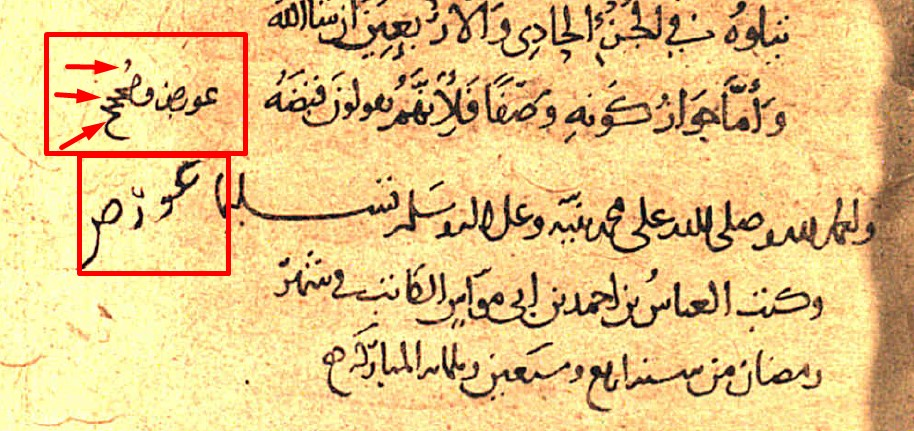
\includegraphics [width=10cm, height=4cm]{SUHIHA.jpg}
    \caption { Exemple d'une marque de collation}
    \label{fig:my_label}
\end{figure}

\begin{figure}
    \centering
    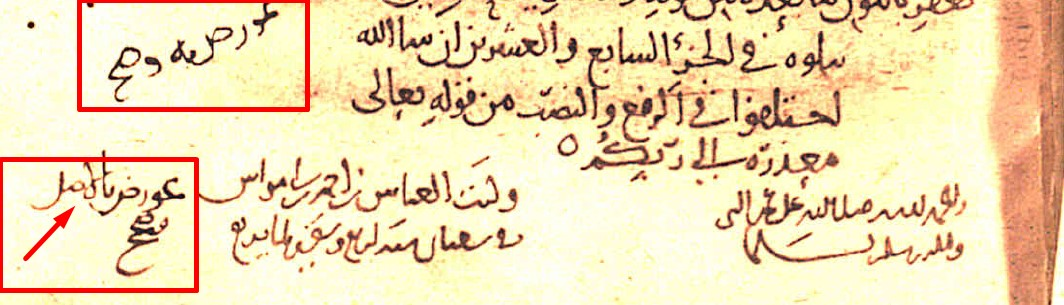
\includegraphics [width=10cm, height=4cm] {bi asl.jpg}
    \caption{Exemple d'une marque de collation}
    \label{fig:my_label}
\end{figure}



















\subsection{	Présentation du manuscrit de la bibliothèque  de Dār al-Kutub al-Miṣriyya, rédigé en 390/999}

Le deuxième manuscrit de notre étude est conservé à la bibliothèque de Dār al-Kutub al-Miṣriyya en Egypte sous la cote 462 
\textit{ qirā ͗ āt  }  Nous l'avons acquis en  copie  photographié en noir et blanc. Il se compose de sept volumes, amputé du cinquième. Les six  volumes consultés ne sont pas complet. des folios manquent  dans divers endroits du manuscrit. 

\paragraph{}
La description précise de la numérotation du Mmanuscrit est impossible pour deux raison : soit par ce que elle figure pas ( la prise de photo n'est pas adéquate)   soit encore par ce  l'état du manuscrit est très dégradé. Toutefois, il faut préciser que le manuscrit porte deux systèmes de numérotation: une numérotation par cahier et une numérotation par bi-feuillet.  

La date d'achèvement est rédigé sur le dernier volume ( volume 7) comme suit ( voir les annexes). 

«\textit{Wa balaġa al-farāġ minh fi yawm al- ḫamīs li-sabʿ baqīn min min ḏī al-qiʿda sanat tisʿīn wa ṯalāṯ miʾa....} »

« La fin de rédaction a eu lieu le jeudi, sept jours avant la fin du mois de \textit{ḏī al-qiʿda} ( le 11ème mois de l'année hégirienne)  de l'an 390...»

Autrement dit, la date de fin a eu lieu vers 2 octobre de l'année 999 en calendrier grégorien. Le lieu de copie et le nom du copiste ne sont pas mentionnés. Le manuscrit comporte des gloses marginales et des ajouts dans différents endroits.


\subsection{ Présentation du manuscrit de la bibliothèque du Murad Molla, rédigé en 427-428/1035-1036 }

Ce manuscrit en quatre volumes est conservé à Murat Molla Kütüphanesi ( la bibliothèque de Murad Molla ) à Istanbul, Turquie, sous le numéro d’ordre 297.1. 6,7,8,9. Nous avons acquis une copie numérisée  microfilm.
\paragraph{}
Le premier folio de chaque volume  indique le titre de l’œuvre. Le  dernier folio fait mention des informations suivantes : la date, le lieu d’achèvement de copie  et le nom de copiste qui a réalisé le travail \footnote{voir la première partie de notre édition (texte ci-joint)}. L’organisation des quatre volumes est  reliée et contrôlée d’une part,  par un contenu homogène. De l’autre part, par une  unité codicologique. Le  desinet \footnote {Le desinit désigne dans le dictionnaire de Muzerelle : « derniers mots d'un texte. ». Pour plus de détail sur le desinit voir également :  Troupeau Gérard. \textit{Les colophons des manuscrits arabes chrétiens}. Dans, Déroche F., Richard, F. \textit{Scribes et manuscrits du Moyen-Orient}, Paris, Bibliothèque nationale de France, 1997, pp. 224-231.} qui figure à la fin de chaque volume indique clairement cet aspect unitaire. En effet, le copiste de l’œuvre arrive, grâce au desinit, à maintenir le fil conducteur entre les quatre volumes par des formules qui annoncent la fin d’un volume et le  début du  volume suivant. 

\begin{itemize}
    \item  	Vol. n 1: a la a fin du premier volume est écrit : la fin du premier volume, que Dieu soit loué, en Égypte  de l’an mille sept ( 427 si on considère les autres volumes). Il sera suivi de \textit{yatlūh} dans le deuxième volume ...
    
    Le nom de copiste est Tāḥar b.Ġalbun le grammairien égyptien . Il est écrit d'une main différente. 
    
    \item Vol. n 2 : a la a fin du deuxième volume est écrit :  que Dieu soit loué. Il a été rédigé \textit{( katabahu ) } Ṭāhar b. Ġalbun \footnote{Les ratures et suppressions, clairement identifiables, laissent penser que  Tāḥar b.Ġalbun  n’a pas rédigé l’œuvre ou son nom a été supprimé et a été réécrit.   Voir les annexes .} en Égypte. La fin de rédaction ( \textit{faraġa minhu} ) en \textit{d̠ī al-qiʿda }[le 11ème mois de l’année hégirienne] de l’an 427. Il sera suivi ( \textit{yatlūhu} ) dans le troisième volume ..... 
    %%%%%%%%%%%%%vol3 
   
    \item 	 Vol n 3: a la a fin du troisième volume est écrit :  que Dieu soit loué. Il a été rédigé ( \textit{katabahu} )  Ṭāhar b. Ġalbun\footnote{De la même façon que le volume précédent, les ratures et suppressions , clairement identifiables, laissent penser que  Tāḥar b.Ġalbun  n’a pas rédigé l’œuvre ou son nom a été réécrit. Voir les annexes } en Égypte. La fin de rédaction ( \textit{faraġa minhu} ) en \textit{d̠ī al-ḥiǧǧa} [le 12ème mois de l’année hégirienne], le deuxième jour [...]  de l’an 427 . Il sera suivi dans le quatrième volume de …. 
 %%%%%%%%%%%%%%%%Vol4
 \item vol. n 4 : a la a fin du quatrième  volume est écrit :  Ceci est  le dernier [volume] de \textit{Kitāb al-huǧǧa}. que Dieu soit loué, prières à son prophète Moͅhamaed et, à  sa famille  . Le mois de \textit{Muḥaram} [1er mois de l’année hégirienne], Le jour de 
\textit{ʿāšurāʾ} [ Le 10  du Muḥaram]  de l’an 428\footnote{Après la fin du colophon, nous pouvons constater  plusieurs ratures et suppressions de mots.  Une main différente a écrit le suivant : Ce livre est en quatre volumes, il est complet. Il a été rédigé par la main (\textit{ ḫat} ) Ṭāhar b. Ǧalbun.  À côté de cette mention, nous lisons :  \underline{hād̠ā h̬at} ibn [ al- bunī/al-buwayn] }. Ce qui est sûr pour nous c'est que le copiste de l'œuvre est soit Ṭāhar b. Ǧalbun comme indiqué, soit l'attribution a ce copiste est fausse, soit encore le nom de copiste a été supprimé puis réécrit. 
\paragraph{}

Il a fallu donc 4 mois consécutifs  pour accomplir  entièrement le travail de copie des quatre volumes.  Les quatre mois chevauchent entre deux ans : 427/1035 et 428/1038. Contrairement aux trois premier volumes, la formule fin de rédaction du dernier volume est  écrite sous forme complète :  le jour, le mois et l’année.  
La mention du jour de \textit{ʿāšurā ʾ} [ Le 10  du Muḥaram]  n’est pas fortuite, elle est une façon symbolique de célébrer, la fin de rédaction et, en même temps, ce jour sacré dans la culture religieuse musulmane.   
\paragraph{}
Le Manuscrit  [M]est numéroté de deux façons très différentes : numérotation des cahiers et numérotation des bifeuillets. La première façon est sous forme d’une réclame \footnote{Selon Denis Muzerelle une réclame est: indication des premiers mots de la page suivante inscrite au bas d’une page , le plus souvent à la jonction entre deux cahiers, permettant de contrôler la bonne succession des feuillets  ou cahiers. Denis Muzerelle,\textit{ op.cit.} p. 113.  } apposée en haut du cahier et écrite  en  lettres arabes.  La deuxième façon  est  tardive car écrite par un crayon  est indiquée en  chiffres arabes et en chiffres indiens. Ci-après une illustration dès deux systèmes de numérotation: 

\end{itemize}
\newpage
\begin{itemize}
    \item •	Vol. n°1 : 
    \begin{itemize}
        \item 	Les cahiers : \textit{ṯānī awal, ṯāliṯ awal}…etc ce qui correspond à ( le deuxième cahier du premier volume, le troisième cahier du premier volume…etc ). 
        \item Les bifeuillets : 
        \begin{enumerate}
            \item La numérotation en chiffre arabe : commence du chiffre 2, 3, 4…etc jusqu’au chiffre  241. 
            \item La numérotation en chiffres indiens : différente
              
          
     
        \end{enumerate}
    
     
        
    \end{itemize}
    \item •	Vol. n°2 : 
    \begin{itemize}
        \item 	Les cahiers : \textit{rābiʿ ṯānī, ḫāmis ṯānī…}etc ce qui correspond à (  le quatrième cahier du deuxième volume, le cinquième cahier du deuxième volume…etc) 
        \item Les bifeuillets : 
         \begin{enumerate}
            \item La numérotation en chiffre arabe :  commence du chiffre 2, 3, 4…etc jusqu’au chiffre  231. 
            \item La numérotation en chiffres indiens : différente
              
         
     
        \end{enumerate}
    
    \end{itemize}
    \item •	Vol. n°3 : 
    \begin{itemize}
        \item 	Les cahiers : \textit{ṯānī ṯāliṯ, ṯāliṯa ṯāli̠ṯ}…etc ce qui correspond à (  le deuxième cahier du troisième volume, le troisième cahier du troisième volume…etc ) 
        \item Les bifeuillets : 
         \begin{enumerate}
            \item La numérotation en chiffre arabe :  commence du chiffre 2, 3, 4…etc jusqu’au chiffre  248. 
            \item La numérotation en chiffres indiens :différente



        \end{enumerate}
    
    \end{itemize}
    \item •	Vol. n°4 : 
    \begin{itemize}
        \item 	Les cahiers : \textit{ṯānī rābiʿ, ṯaliṯ rabiʿ}ᶜ…etc ce qui correspond à ( le deuxième cahier du quatrième volume, le troisième cahier du quatrième volume…etc ) 
        \item Les bifeuillets : 
         \begin{enumerate}
            \item La numérotation en chiffre arabe : il commence du chiffre 2, 3, 4…etc jusqu’au chiffre  257. 
            \item La numérotation en chiffres indiens : différente    \footnote{Il faut souligner que nous avons indiqué la numérotation ci-dessus à titre indicatif. Nous avons constaté que dans divers endroits les numérotation présentent des anomalies ( numérotation par feuillet au lieu de bifeuillet, ratures, répétitions et autres erreurs.) La vérification minutieuse et la prise de compte de toutes ces anomalies dépassent le cadre de ce travail.  }
     
        \end{enumerate}
    
    \end{itemize}
Chaque feuillet du manuscrit [mīm] comporte  environ 18 ligne. Une seule ligne compte en moyen 10 mots. La réglure  est  bien justifiée  avec des notes, corrections, ajouts  sur les marges.  
Le texte est intégralement diacritisé et vocalisé avec quelques voyelles et des points diacritiques de plus ou en moins dans divers endroit. D’une façon globale, le copiste semble un connaisseur du travail de copie voir même un professionnel de l’art de l’écriture. 

L’ensemble de l’œuvre a fait l’objet d’une collation par volume.  Les expression de collation sont:

\begin{itemize}
    \item •	Vol. n°1 : pas de marque de collation visible. 
    \item •	Vol. n°2 : à la fin du volume est écrit : \textit{qūbila bih fa-ṣaḥḥa in šāʾ allāh} ( Il a été collationné et [ devenu] correcte si Dieu le veut.
    \item •	Vol. n°3 : à la fin du volume est écrit : \textit{qūbila bih fa-ṣaḥḥa in s šāʾ allāh} ( Il a été collationné et [ devenu] correcte si Dieu le veut. 

    \item •	Vol. n°4 : Sur l’avant dernier feuillet. Après le dernier mot de fin, il est écrit:  \textit{qābaltuhu ǧamīʿuhu fa-ṣaḥḥa in šāʾallāh} ( Je l'ai  collationné et [  devenu] correcte si Dieu le veut. L'expression \textit{ǧamīʿuhu} ( le tout ) peut renvoyer à l’ensemble de l’œuvre comme elle peut également  désigner le seul volume n°4. 


\end{itemize}

    
\end{itemize}
\newpage
\subsection{ 	Présentation du manuscrit de la bibliothèque de Feyzullah, rédigé en 642/1244  }

Le dernier  manuscrit dans la chronologie de rédaction des manuscrits de notre étude  est conservé à la bibliothèque de Feyzullah à Istanbul en Turquie sous la cote n : 3. Il est amputé de plusieurs parties, la partie qui a subsisté ( au moins jusqu'à la rédaction de ces lignes)  est le troisième volume. Nous l'avons acquis en format numérisé microfilm 

Ce volume semble être le dernier de l'ensemble de l'œuvre car d'une part, il se clôt sur la dernière sourate du Coran (114) \textit{al-Nās}. De l'autre part, il est  écrit à la fin du volume: le nom du copiste, la date de fin de copie (le deuxième mois de l'an 642) et le lieu : la ville de Damas en Syrie comme suit :  
\begin{center}
    
\textit{
Tamma kitāb al-ḥuǧǧa [….] wa faraġa min taḥrīrīhi al-faqīr [...] al-rāǧī ʿafwa allāh Abū ʿAbd allāh Moḥamed b. Aḥmed b. Aby Bakr b. H̬alīl al-Mazd̠aqānī […] bi Madīnat Dimašq […] en safar} [le deuxième mois de l’année hégirienne] \textit{h̬atamahu allāh bi al-h̬ayr sanat it̠nayn wa arba ʿīn higriya nabawiyya.}. 

\end{center}
    
Nous n'avons  trouvé aucune information ou renseignements  sur le copiste de l'œuvre: Abū ʿAbd allāh Moḥamed b. Aḥmed b. Abū Bakr b. Ḫalīl al-Mazḏ̠aqānī.

\paragraph{}
 Sur La page de titre figure plusieurs notes  de possession ce qui indique clairement que ce manuscrit a fait l'objet  d'un usage  soit collectif tel que  des enseignements  de \textit{ samaʿ̄} (lecture-audition)   soit encore un usage  particulier tel que   \textit{munāwala}  (  remise )  ou    \textit{iǧāza} ( licence/autorisation de transmission )\footnote{ Pour plus d'informations sur ces procédés de transmission de savoir religieux en terre  d'Islam. Voir la suite de e travail: partie édition et le dernier chapitre de ce mémoire}       

Au début, fin et milieu le Ms [F] il y a  des mentions de  \textit{waqf} écrites  en gros caractères.  Toutefois, aucune précision sur le donateur, ou l'institution  qui abrite ce \textit{waqf} ou la date...etc. (voir première figure ci dessous) 

Probablement, Il s'agit d'un \textit{waqf} ottoman  légué ou collecté par l'école du savant ottoman Fayḍ allāh.  Un sceau rond au début et à la fin  du volume précise le suivant: (voir l'édition et la traduction du contenu et la figure 2 ci-dessous) 

\textit{
Waqf šayḫ  al-islām al-sayyīd Fayḍ allāh afandī ġafara allāhu lahu wa li-wālidayhi bi-šart ʾan lā yah̬ruǧa min madrasatihi bi al-qustantīniya sanat 1112.} 

(\textit{waqf}  au nom de \textit{šayḫ  al-islām} [titre honorifique et officiel] ̄monsieur  Fayḍ allāh afandī. Que le bon Dieu lui pardonne  ainsi que ses parents, à condition que [ce livre] ne sort pas de l'école qu'il a fondé à constantinople en 1112 [ une date de hégire sans aucun doute. 1700 en grégorien]


\begin{figure}
    \centering
    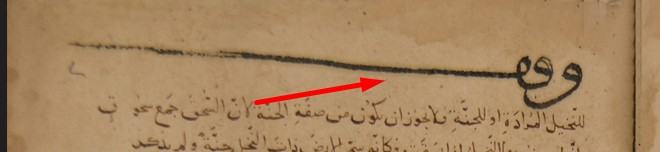
\includegraphics [width=10cm, height=4cm]{acte de waqf.jpg}
    \caption {Exemple d'une marque de \textit{waqf} écrite à la main }
    \label{fig:my_label}
\end{figure}
\begin{figure}
    \centering
    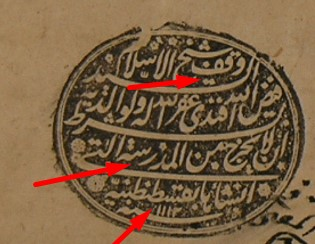
\includegraphics [width=10cm, height=4cm]{waqf fayzullah.jpg}
   \caption {Exemple d'une marque \textit{waqf}  en forme de sceau rond}
    \label{fig:my_label}
\end{figure}
 




La numérotation du Ms de la bibliothèque de la bibliothèque de Feyzullah est tardive ( écrite par un crayon). Il s'agit d'une  numérotation par bifeuillet ( successivement du  chiffre 1 au  chiffre 249). Chaque feuillet comporte environs 20 et 25 ligne, environ 10 mots par ligne.

L'écriture et trop serrée, entièrement vocalisée avec quelques omissions et oublies de voyelles et signes diacritiques. l'auteur a  rédigé les parties importantes en gros caractères. 
\newpage
\subsection {Présentation de l'édition imprimée de Damas }


L'édition imprimée de \textit{kitāb al-ḥuǧǧa } que nous avons utilisé lors de notre travail est éditée par Badr al-Dīn Qahwaǧī et al.̄ \footnote{ al-Fārisī abū ʿAlī, \underline{ al-ḥuǧǧa li-lqurāʾ al-sabaʿa}, (éd) Badr al-Dīn Qahwaǧī et al, Damas,  Dār al-maʾmūn li-turāṯ  1974.} Publié pour la première fois en 1974. L'apport princiapl de cette édition est de donner accès à une oeuvre majeure sur les Variantes de lecture. L'autre qualité de cette édition est le volume spécial consacré aux indexes : riche, divers et logiquement structuré.   Toutefois, les choix éditoriaux, philologique ...etc restent discutable.   
\paragraph{}
L'édition s'ouvre  par une longue introduction (45 page), presque dogmatique. Le premier tiers  reprend scrupuleusement  la conception théologique musulmane des Variantes de lecture.  Les deux autres tiers ont été consacrées à  la présentation de l'auteur, son œuvre  et une brève  description des manuscrits. L'importance des certificats de lecture-audition, les mentions de possession et les licences de transmission pour l'histoire du texte n'a pas vraiment retenu l'attention des éditeurs voire même sous-estimé.   

Les éditeurs se sont basés sur deux copies manuscrites.

\ding{202} La première est désignée par la lettre arabe \begin{Arabic}
  \Large  {م}
\end{Arabic}  (=  [k] dans notre présente édition)

\ding{203} Et la deuxième copie manuscrite est désignée  par la lettre arabe \begin{Arabic}
   \Large {ط}
\end{Arabic}(= [M] dans notre présente édition)
\paragraph{}
Le texte de base de l'édition imprimée de Damas  est le manuscrit tardif (manuscrit  \begin{Arabic}
  \Large  {م}
\end{Arabic} rédigé vers 427. Pour le lecteur,  ce choix reste injustifié  dans l'introduction des éditeurs. Pour nous (éditeur)  nous pouvons déduire  que ce choix est  motivé par le caractère  achevé du  manuscrit  \begin{Arabic}   
  \Large  {م}
\end{Arabic}. Autrement dit, dans la la classification des manuscrits les éditeurs ont préféré la complétude du manuscrit \begin{Arabic}
  \Large  {م}
\end{Arabic} au lieu du Ms le plus proche de l'archétype, du texte original .     

\paragraph{}
L'apparat critique  des éditeurs  ne comporte que les  variantes\footnote { Pour un lecteur peu habitué à la discipline  de \textit{ qirāʾāt} ,   le terme \textit{Variante} dans le sens de l'édition critique des textes  peut être facilement confondu avec  l'expression technique \textit{Variante de lecture} tel que entendu   par tradition musulmane. 

Nous tenons à les distinguer au cours de ce travail par: Variantes de lecture coranique, Variantes de lecture ou  \textit{ qirāʾāt}. Le terme \textit{Variante} tout seul renvoie à la variante tel que entendu par la tradition de l'édition critiques dès textes c'est à dire: « Pour une oeuvre donnée, une variante est une différence entre la leçon admise et consignée par l'éditeur ou l'auteur et une autre leçon présente sur un document de genèse ou dans une autre édition ou version de la même oeuvre. Il peut s'agir aussi bien d'une partie de texte de grand dimension que d'un seul mot ou d'un élément plus infime encore.»  Breuil Eddie,\textit{Méthodes et pratiques de l'édition  des textes et documents modernes}, Paris, classiques garnier, 2019, p. 859.  

Pour la définition d'une variante de lecture  dans la tradition musulmane ( voir le premier chapitre de ce travail.)}  les plus évidentes. Les éditeurs de l'œuvre intègrent dans  l'apparat critique  \textit{ kitāb al-sabʿa} de Ibn Muǧāhid et autres œuvres de \textit{tafs\=ir},  de grammaire ...et. Si ce choix peut être compris, il  reste injustifié dans l'introduction. 

 
\subsection{ Un Manuscrit de  \textit{kitāb al-ḥuǧǧa}, identifié, localisé et non accessible  }

Lors de la première étape de ce projet de recherche ( la collection des  manuscrites) nous avons identifié une copie de \textit{ kitāb al-ḥuǧǧa }en Inde mais, nous n'avons pas pu avoir accès à cette copie  pour diverses raisons. Cela n'empêche pas de donner les quelques informations que nous détenons  sur ce manuscrit. Tout ce qui vient se base seulement sur le catalogue de la bibliothèque. 

\paragraph{}

Le manuscrit en question est conservé à la bibliothèque de  Khuda Bakhsh Oriental Public, province de patna en Inde sous le numéro de cote 1210. Khuda Bakhsh est un haut fonctionnaire indien né le 2 Août 1842 et mort en 1908. 
La bibliothèque contient un nombre considérable  de manuscrit (plus 21000) dans plusieurs langues : arabe, persan, turque ...etc.  et dans tous les domaines du savoir ( le Coran, \textit{tafsi\=ir,} langue et philologie, théologie, médecine...etc. Parmi les précieuses acquisitions de la  bibliothèque un exemplaire du Coran en 256. fol écrit en  style \textit{kuf\=i}. datable au IX/ème siècle selon l'auteur du catalogue. 

Quant à notre manuscrit \textit{kitāb al-ḥuǧǧa }de al-F\=aris\=i, il est en deux volumes, la date de copie n'est pas indiquée mais, la confrontation de ce que rapporte l'auteur du catalogue et les certificats de lecture-audition (\textit{sam\=aʿ\=at}) que nous avons édités ( voir l'édition est la dernière partie de ce travail) permet de dire que le manuscrit de l'inde a circulé en Syrie à la fin du VI et le début du VIIème siècle.  En effet,  Le manuscrit  de  la bibliothèque de  Khuda Bakhsh Oriental Public contient des certificats de lecture-audition authentifié par  Ab\=u Zayd al-Kind\=i (né.520/1125- m. 613/1216)  et  de la même date et lieu que notre  manuscrit [M] :  606/1209 à l’école al-ʿAzīziyya à Damas. \footnote{ Voir les catalogues , toutes les informations citées et autres sur: \url{ https://kblibrary.bih.nic.in/default.htm } dernière consultation le 23 août 2022} 




\newpage
\begin{french}
    

\section{Les principes de l'édition }

L’essence du travail de l’édition critique des manuscrits est basé sur le principe fondamental de choix et de privilèges établis par l’éditeur scientifique d’une œuvre. La multiplicité des copies, l'état général des copies , les variantes de chaque copie et autres obstacles obligent celui qui édite un manuscrit à se résigner à la loi  de l’adoption et du rejet.  Choisir et privilégier est donc une partie inséparable de l’édition. Dès lors, la principale tâche de l’éditeur scientifique d’un manuscrit est d'abord identifier les manuscrits à éditer, ensuite déterminer et estimer les différences entre les copies manuscrites et finalement rendre compte et  justifier à son lecteur les leçons et variantes retenues et celles qui ont été  rejetées  ainsi que  toute autre intervention  quelle qu’elle soit. En outre, il doit d’une part respecter  les exigences philologiques et éditoriales  de l’édition critique des textes et, de l’autre part se conformer aux  attentes du lecteur. L’éditeur scientifique est un medium qui doit « chercher à concilier le respect des éléments qui peuvent être signifiants et les commodités fournies au lecteur moderne.»\footnote{Vielliard Françoise et Guyotjeannin Olivier, \textit{Conseils pour l’édition des textes médiévaux fascicule I : conseils généraux,} Paris, École nationale des chartes, 2014, p.75. }
\paragraph{}
Il est d’usage dans le domaine d’édition des manuscrits médiévaux dans toutes les aires culturelles et linguistiques d’accompagner le texte édité par une introduction  dite :  introduction de l’éditeur ou introduction à l’édition. Celle-ci a pour fonction et objectif de donner accès au texte ou document édité et de rendre tous les choix ou les objections faites par l’éditeur aussi explicite que possible. Toutefois, les éléments et aspects abordés dans l’introduction  dépendent de l’intérêt, le publique visé, le domaine…etc. Ainsi, certains  éditeurs scientifiques préfèrent retracer l’histoire du travail en entier, du premier contact avec les manuscrits jusqu’à la publication finale du travail. D’autres  consacrent une grande partie à la présentation de l’auteur, de  son œuvre et son apport, éventuellement le contexte intellectuelle et historique. En bref,  les parties suivantes doivent être présentes dans une édition : la description des manuscrits, la méthode de suivie et le choix du manuscrit de référence.

\newpage
\subsection{Le Manuscrit de base et les sigles utilisés pour la ré-établissement du texte}


C’est le manuscrit [A] qui nous a servi de texte de base pour l’édition de la \textit{sourate} . Bien que lacunaire nous avons estimé que [A]  est l’idéal comme texte de base pour diverses et multiples  raisons. 

\paragraph{}
\textbf{En premier}, L’analyse des colophons et les titres  nous a montré la supériorité et  caractère ancien de ce manuscrit. Comme dit dans la présentation des manuscrits, il a été rédigé vers 374 de l'hégire ce qui veut dire qu’il a circulé du vivant de al-Fārisī . Il se peut même qu’il soit  copié  directement de l’archétype\footnote{Pour Denis Muzerelle, \textit{op.cit.}  p.141. L’archétype est : Exemplaire -connu ou supposé- dont sont censées dériver toutes les copies subsistants d’un texte.   }  mais, rien ne nous permet d’affirmer cela. En revanche, ce qui est sûr est que ce manuscrit est chronologiquement  le plus proche de l’archétype. 
\paragraph{}

\textbf{Une deuxième raison} du choix  du manuscrit [A]  pour l’édition est la comparaison du travail des quatre copistes. En effet, lors  du travail préparatoire et pré -éditorial ( la transcription et la comparaison des copies)  nous avons relevé certains traits dans le  manuscrit [A] qui ont été repris dans les autres manuscrits. Ainsi, si on applique la règle de la philologique classique : il est impossible que deux copistes font la même erreur au même endroit nous pouvons  remarquer que d'une part, les corrections et gloses  faites par le copiste de [A] ( ou un lecteur du manuscrit)  sur la marge intègrent directement le corps des autres manuscrits. De l'autre part, certains signes du manuscrit [A] ont été aussi repris dans les trois autres manuscrits. (voir l'apparat critique)

\ding{242}	Les corrections rédactionnelles:\footnote{Denis Muzerelle,  \textit{op. cit.} p. 121. Définit une  correction rédactionnelle  ainsi: correction destinée à modifier intentionnellement le contenu, le sens ou les caractères formels du texte et non pas à corriger seulement une faute ou une incorrection.  }  et les notes marginales, gloses et ajouts  du manuscrit [A] intègrent le  corps du texte des trois autres manuscrits. par exemple ( note de bas de page: 58 , 61, 92, 260). Sans le manuscrit [A], le lecteur comprendra qu'il s'agit de mots/phrases qui font partie du texte original alors qu'il s'agit d'ajouts et de corrections du copiste ou des lecteurs. 
 Autant de variantes dans l'apparat critique de la sourate indiquent clairement que nos trois autres manuscrits ont suivi  le manuscrit [A], soit directement soit encore,  indirectement par un ou plusieurs manuscrits intermédiaires . 

\ding{242}	Les signes de ponctuation et de repère  : il est bien évidant qu'employer le terme  de ponctuation pour un texte médiéval  est anachronique. La ponctuation actuelle de l'arabe ( qui est aussi celle des autres langues) est introduite vers la fin du  XIXème siècle et le début du XXème siècle. Toutefois, nous constatons que dans plusieurs endroits de  nos quatre manuscrits les copistes marquent une pause par un signe particulier ( voir les illustrations  ci-après). 

En toute logique,  les signes remontent au manuscrit [A] car il est le plus ancien dans notre corpus. Il se peut aussi que ces signes  font partie de l'archétype ou un autre ( ou plusieurs) manuscrit intermédiaire perdus  qui se situent notre notre manuscrit de base [A] et l'archétype, entre 374 de l'hégire et la date de la première rédaction de  \textit{Kitāb al-ḥuǧǧa}. Ainsi, Ceux qui ont rédigé après le manuscrit [A] n'ont, à vrai dire, que recopier servilement et des fois maladroitement. 

\begin{figure} [H]
    \centering
    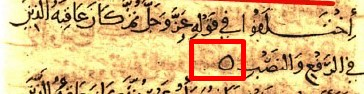
\includegraphics [width=8cm, height=1cm]{Ms A ponctuation 1.jpg}
    \caption{Manuscrit [A], Marque de ponctuation au début de la sourate éditée}
    \label{fig:my_label}
\end{figure}

\begin{figure} [H]
    \centering
    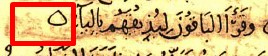
\includegraphics[width=8cm, height=1cm]{Ms A ponctuation 2.jpg}
    \caption{Manuscrit [A], Marque de ponctuation à la fin de la sourate éditée}
    \label{fig:my_label}
\end{figure}

\begin{figure} [H]
    \centering
    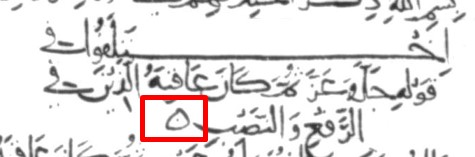
\includegraphics [width=8cm, height=1cm] {Ms K-ponctuation1.jpg}
    \caption{Manuscrit [K], Marque de ponctuation au début de la sourate éditée}
    \label{fig:my_label}
\end{figure}

\begin{figure} [H]
    \centering
    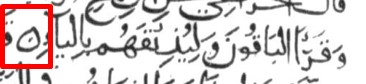
\includegraphics [width=8cm, height=1cm] {Ms K-ponctuation 2.jpg}
    \caption{Manuscrit [K], Marque de ponctuation à la fin de la sourate éditée}
    \label{fig:my_label}
\end{figure}

\begin{figure} [H]
    \centering
    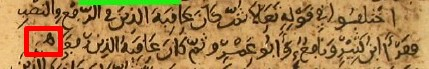
\includegraphics [width=8cm, height=1cm]{MS M ponctuation 1.jpg}
    \caption{Manuscrit [M] Marque de ponctuation au début de la sourate éditée}
    \label{fig:my_label}
\end{figure}

\begin{figure} [H]
    \centering
    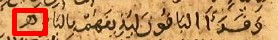
\includegraphics [width=8cm, height=1cm]{MS M ponctuation 2.jpg}
    \caption {Manuscrit [M] Marque de ponctuation à la fin de la sourate éditée }
    \label{fig:my_label}
\end{figure}


\begin{figure} [H]
    \centering
    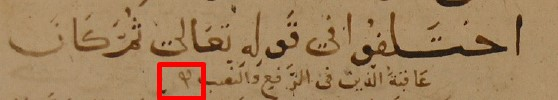
\includegraphics [width=8cm, height=1cm] {MS F ponctuation 1.jpg}
    \caption{Manuscrit [F], Marque de ponctuation au début la sourate éditée }
    \label{fig:my_label}
\end{figure}

\begin{figure} [H]
    \centering
    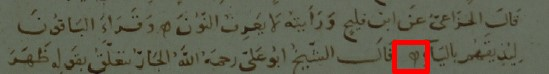
\includegraphics [width=8cm, height=1cm]{MS F ponctuation 2.jpg}
    \caption{Manuscrit [F], Marque de ponctuation à la fin de la sourate éditée}
    \label{fig:my_label}
    
\end{figure}


Les  éditeurs confirmés font la différence entre une simple variante (généralement graphique)  et une leçon qui peut impacter sensiblement le sens et la cohérence d'un mot, une phrase ou un texte entier. Voici quelques exemples de variantes et de leçons tirées de notre édition :


\begin{figure} [H]
    \centering
    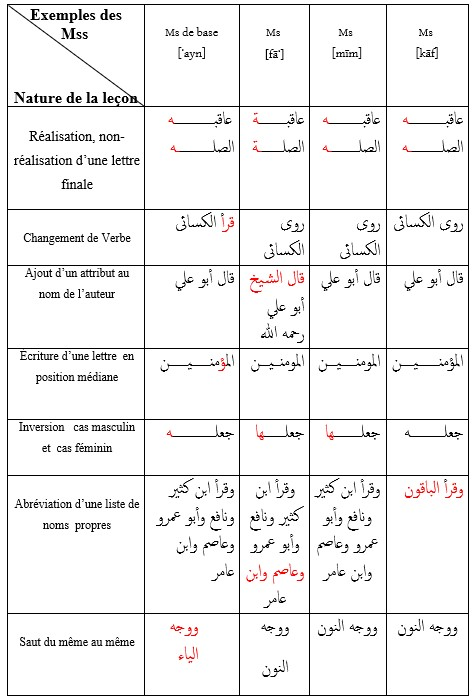
\includegraphics [width= 14cm, height=15cm]{Leçons 1.jpg}
    \caption{ Exemple de quelques leçons et variantes  }
    \label{fig:my_label}
\end{figure}

\newpage
Par convention de langage, nous employons les sigles ci-après pour désigner : 

\begin{enumerate}
    \item 
Manuscrit de la bibliothèque de  Ali Paşa, rédigé en 374/984 =  [A] /
\begin{Arabic}
 \Large ع 
\end{Arabic}
  \item Manuscrit de la bibliothèque de Dār al-Kutub al-Miṣriyya, rédigé en 390/990= [K] /
\begin{Arabic}
 \Large ك 
\end{Arabic}

  \item Manuscrit de la bibliothèque du Murad Molla, rédigé en 427-428/1035-1036  [M] /
\begin{Arabic} 
\Large
م 
\end{Arabic}
  \item  Manuscrit de la bibliothèque de Feyzullah,
rédigé en 642/1244 = [F] / 
\begin{Arabic}
\Large
 ف
\end{Arabic} 

 \item Exclusivement dans l'édition nous avons utilisé le sigle   
\begin{Arabic}
\Large
 مص = مصحف
\end{Arabic}
Pour noter dans notre apparat critique les versets tels que figurent dans le \textit{muṣḥaf}.
Exemple :

\begin{Arabic}
الروم، 10 [مص]= ثُمَّ كَانَ  عَٰقِبَةَ ٱلَّذِينَ أَسَٰٓـُٔواْ ٱلسُّوٓأَىٰٓ
 \end{Arabic}
 
 Veut dire: sourate al-Rūm, verset 10, dans le \textit{muṣḥaf} est... 
    

\item 	Les crochets [ ]   nous ont servi aussi à indiquer quelques amendements. 

\item  Les crochets avec trois points  à l'intérieur […] pour montrer que le mot est illisible dans le manuscrit.



\end{enumerate}

 








\newpage
\begin{french}
    

\subsection{Notes sur le processus  de l’édition du texte de la sourate}

Le passage d’un texte manuscrit à un texte imprimé est une étape de modernisation et de conservation d’un texte. L’éditeur scientifique qui accompagne, par son travail d’édition, ce passage doit veiller à la présentation  du contenu et de  la forme. Le choix d'un manuscrit de référence ou le signalement des leçons et variantes dans l'apparat critique n'est pas souvent suffisant. Le manuscrit de base n'est pas exempte d'erreurs, omissions...etc.  Dès lors comment procéder pour rendre un texte le plus authentique possible à l'original ?

Il y a  trois méthodes (possibilités) 
\begin{itemize}

\item Il y a des éditeurs qui préfèrent alterner les manuscrits  pour retenir la leçon la plus correcte, 
\item Il y a ceux qui soulignent dans l’introduction de l’édition les amendements et améliorations faites dans un tableau ou dans une liste ou par nombre. 
\item Il y a ceux qui contentent de souligner les amendements par des appel de notes dans l'apparat critique. 
    
\end{itemize}

Nous avons choisi cette dernière méthode pour souligner toutes les amendements ou erreurs dans notre manuscrit de base. 
\paragraph{}
Un des problèmes majeurs de la bonne compréhension des auteurs médiévaux est un  écart double : linguistique et stylistique d’une part, intellectuel et historique de l’autre. Ainsi, certains passages ou phrases peuvent paraître comme incomplètes et insignifiantes ou une digression,  ce qui crée des problèmes d’interprétation et des conflits sémantiques à l’intérieur du texte ou d'une phrase.  Comment pallier, du moins réduire, cet écart  et  fournir un accès moins linéaire  au texte ? Nous avons  :

•   Numéroter les passages contenant des variantes de lecture dans le texte édité. 

 •  Les versets coraniques ont été mis entre  parenthèse ornées.

 • Au lieu de paragraphes formels, nous avons préféré des paragraphes sémantiques  pour faciliter la lecture. Autrement dit, on divisé autant que possible le texte en paragraphes qui ont une unité sémantique. 

• Quand c'est nécessaire, nous avons ponctué le texte. 

• Les vers de poésie dans l'édition ont été édités selon la façon classique\textit{ ṣadr} (première partie)  et \textit{ʿaǧz } (deuxième partie)

• Nous avons donné un titre à chaque chapitre, sauf le chapitre de la \textit{sourate} où le titre   figure dans le manuscrit. La \textit{basmala}  fait partie aussi des manuscrits.  
 

\end{french}
 
\subsection{La méthode de l’édition des éléments péri-textuels}

L’édition des éléments péri-textuels\footnote{Nous entendons par éléments péri-textuels toutes les annotations inscrites sur le manuscrit [M] mais,  ne font pas partie du contenu intellectuel.  Ils sont au nombre de trois: les certificats de lectures-audition \textit{samāʿat} les mentions de possessions et les licence de transmission \textit{iǧāzāt }}.
n’obéit pas au mêmes règles que le texte de la\textit{ sourate} pour plusieurs raisons.  La  forme, la date de rédaction, la fonction et et la finalité de ces éléments est différente du contenu intellectuel proprement. Les éléments péri-textuels ne sont pas prévus dans le projet initial de l'auteur.  La question que nous avons posé au départ est: comment éditer ces éléments ? et comment faciliter  l'exploitation de leur contenu dans notre travail?  

Nous avons parcouru  quelques  textes édités pour trouver une méthode idéale  afin d'éditer  ces éléments disparates. Nous avons constater que chaque chaque éditeur procède d'une façon différente de l'autre en fonction des objectifs de chacun et qu'il n' y a pas forcément une méthode suffisamment aboutie  pour éditer ces éléments. Dès lors, nous avons préféré questionner le contenu des éléments et les classer d'une façon logique. En bref,  rassembler les éléments homogènes et  séparer les éléments hétérogènes. 

Pour chaque volume \textit{ǧuzʾ} (on a quatre) du manuscrit [M], nous avons retenu trois grandes parties : les certificats de lecture-audition, Les notes et mentions de possession et les licences de transmission. Selon le volume et le contenu,  nous avons divisé chaque grande en sous-partie comme suit :

\begin{enumerate}
    \item \textbf{les certificats de lectures-audition \textit{samāʿa} }: ils diffèrent selon le contenu en :
    \begin{enumerate}
        \item Certificat de lecture-audition  individuel : Le contenu de ce type de certificat concerne une seule personne. 
        
      \item Certificat de lecture-audition  collectif:      Le contenu de ce type de certificat concerne plusieurs personnes 
        
    \end{enumerate}

\item    \textbf{Les notes et mentions de possession : } ils diffèrent selon la formule de possession employée  en : 
\begin{enumerate}
    \item  formule possession explicite et bien connue : ce qui indique que la personne concernée a bien acquis \textit{ kitāb al-Ḥuǧǧa} soit l'ouvre entière ou un seul volume  d'une façon ou d'une autre ( achat, acte de \textit{waqf}, héritage successoral, don ...etc)
\item Absence de formule de possession : ce qui veut dire que la personne a eu un contact avec l'œuvre  (\textit{Kitāb al-Ḥuǧǧa}) sans que le mode de contact soit  suffisamment identifié pour nous.  Il se peut qu'il s'agit d'une personne qui a participé aux enseignements, emprunter,  acquis ..etc l'ouvre entière ou un seul volume. Il se peut aussi qu'il s'agit d'une simple inscription de curiosité ( un nom volant) car le livre est un objet précieux et rare à l'époque médiévale.  
    
\end{enumerate}

\item \textbf{les licence de transmission \textit{iǧāza }} : nous avons seulement deux licences de transmission inscrites sur le volume 3 et sur le volume 4. Elles ne sont pas entièrement lisibles. Nous avons donc essayé dans la mesure du possible de reconstituer et commenter les parties lisibles.    
\end{enumerate}

\paragraph{}
Après le classement raisonné  des éléments péri-textuels, il a fallu aussi adopter une démarche qui facilite la consultation et  manipulation de chaque élément péri-textuel et le renvoi explicatif entre notre commentaire et la partie édition. Nous avons alors décider de numéroter les certificats de lectures-audition \textit{samāʿ}
et les les licence de transmission \textit{Iǧāza } selon la même disposition du manuscrit. Autrement dit, chaque  numéro de ligne dans l'édition  renvoie  à une ligne  dans le manuscrit.

Comme on peut constater dans les annexes l'écriture est  défective,  c'est à dire qu'elle est sans vocalisation ni signes diacritiques sauf quelque  cas. En se basant sur les traités biographiques et la littérature secondaire ( voir le chapitre 5 : la transmission, la diffusion de \textit{kitāb al-Ḥuǧǧa  } : essai de reconstruction critique) 

Nous sommes conscients que vocalisé un texte ou  un simple  mot  dans les langues consonantiques  comme l’arabe veut dire forcément  assigner une  prononciation.   

À titre d’exemple dans notre édition le nom propre  al-Kindī ab \=u al-Yumn peut être lu sans vocalisation: al-Kanadī ab\=u  al-Yaman. ( le canadien ab\=u le Yeman ) ce qui est faux. la lecture exacte est  al-Kindī  ( en référence à la ville historique ( et la tribu)  de Kinda au Yeman) et al-Yumn ( la bénédiction et le bien) . Nous assumons donc toute éventuelle erreur.    

En outre, les éléments péri-textuels  de notre édition sont essentiellement des noms propres. D'une façon générale, la référence religieuse, culturelle ou ethnique...etc, l'usage quotidien et la fréquence  sont les règles qui gouvernent le nom propre. Le façon de nommer les personnes n'est pas stable, elle évolue au fil du temps et des géographies. 

 
\paragraph{}
Pour éviter toute erreur,  nous avons mobilisé toutes les ressources nécessaires : la littérature biographique spécialisée ou les données de la langue. Dans certains cas, c'est  l'intelligence de la langue plus que le manuscrit qui permet de déchiffrer. Par exemple, si on lit un mot \textit{wa ʾḫūh} (avec son frère) la suite est forcement une seule personne, \textit{wa ʾḫawāh} ( avec ses deux frères) la suite est forcement deux noms propres, \textit{wa iḫwatih} ( avec ses frères) la suite est sans doute trois noms propres ou plus...etc. La  conjonction de coordination \textit{wa} ( et) nous a aidé pour séparer les unités onomastiques d'un seul nom propre et autres techniques et subtilités.   
   
Ce que nous n'avons pas pu déchiffrer est mis entre deux crochet avec trois points à l'intérieur [...] 

Ce qui est important et aide à la bonne compréhension des éléments péri-textuels    est \textbf{mis en gras} ou \underline{souligné} 
 

\end{french}



\chapter{La partie édition. Voir le texte arabe ci-joint} 

La partie édition contient, par ordre croissant,  les chapitres suivants  : 
\begin{enumerate}
    \item  Le titre donné l'oeuvre dans chaque manuscrit

    \item  Le prologue

    \item L'édition de la sourate al-R\=um

    \item L'édition des certificats de lecture-audition du manuscrit [M] 
    \begin{enumerate}
        \item Vol.I 
        \item Vol.II
        \item Vol.III
        \item Vol.IV
      
    \end{enumerate}

    \item Les notes de possession 
\begin{enumerate}
     \item Vol.I 
        \item Vol.II
        
        \item Vol.III
        \item Vol.IV
\end{enumerate}
    \item Les licences de transmission 

    \begin{enumerate}
        \item Vol.III
        \item Vol.IV
    \end{enumerate}
    \item Annexe(s)
\end{enumerate}







\chapter{	Analyse et commentaire de l'édition }



\section{	Une seule œuvre et des titres multiples : remarques et interrogations}



\textgoth{L}’œuvre qui fait l’objet de ce travail détient  plusieurs dénominations indiquant le  titre de l'œuvre.\footnote {Nous avons édité ces titres : voir le texte arabe chap.1)} Les mots et expressions employées dans chaque manuscrit sont différentes. Certains dénominations  sont abrégées, d’autres plus longues. Il faut noter au prime abord que  d'une manière générale le titre d’un manuscrit peut être conçu par l’auteur d’une œuvre lui-même ou son scribe,  il peut aussi être une pure conception et  création des copistes dans des époques ultérieurs. Quoi qu’il  soit,  un titre doit être représentatif,  suggestif et refléter en peu de mots le contenu d’une œuvre.  Dans notre cas, le titre conventionnel et partagé  par tous les copistes est: \textit{Kit\=ab al-ḥuǧǧa}. Chaque copiste ajoute d'autres informations sur l'auteur, l'oeuvre et l'époque; quelques unes ont retenu notre attention.     

 
\paragraph{}
\textit{al-ḥuǧǧa}(littéralement : l’argument) est un terme issu du lexique et du registre  des  philosophes musulmans  \textit{mutakalimūn-s} et des spécialistes de la loi religieuse musulmane \textit{uṣulite-s }. Il est aussi fortement présent dans   la logique et la dialectique musulmane. \textit{Al-ḥuǧǧa } est une  preuve éclatante et infaillible qui demande une profonde méditation pour être saisie.

Le deuxième terme qui retient l'attention dans les différents titres donnés à l'œuvre est  l'acte même d'écrire et rédiger dit 	\textit{taʾlīf} . Nous constatons un changement sensible dans le lexique employé  selon l'époque de rédaction comme suit :

 \begin{enumerate}
     \item Le Manuscrit le plus ancien ( [A] 374/984) : l'acte d'écrire est dans toutes les sous-parties   dit :	\textit{Sanaʿahu} (littéralement= a été fabriqué  par.. ) 
  \item  Le Manuscrit  [K] 390/999 l'acte d'écrire est dans les six parties  dit	\textit{taʾlīf}.  
    
    \item Le Manuscrit [M] 427-428/1035-1036 : l'acte d'écrire est dans les six parties est dit \textit{taṣnīf} ( classer). En outre,  le copiste du Ms a donné un titre différent du manuscrits [A] et [K].  Les quatre volumes composant le manuscrit [M] portent un titre presque identique et semblable , même si,   on peut constater   que le Vol.  1 trahit légèrement cette unité de titre. En effet, dans le Vol. 1 les lecteurs ( \textit{qurā}ʾ ) sont identifiés comme étant : \textit{qurāʾ al-amṣār} ( les lecteurs des garnisons/provinces ). En revanche, le Vol.  2, Vol. n 3 et le Vol. n 4  sont qualifiés de :\textit{ ʾaimat al-amṣār} ( les \textit{im\=am-s} des garnisons/provinces ). 


     \item Manuscrit [F] 642/1244 l'acte d'écrire est dit	\textit{taʾlīf} Le titre est très abrégé ce qui montre que le(s) destinataire(s) de ce manuscrit connaît l'œuvre et l'auteur.

     Selon le Manuscrit et l'époque, nous avons trois mots pour désigner l'acte d'écrire dans la culture musulmane : \textit{Sanaʿa} et \textit{taʾlīf}, \textit{taṣnīf}.  Le  terme qui subsiste jusqu'à nos jours est \textit{taʾlīf}.  
 \end{enumerate}

\paragraph{}
Le troisième terme qui attire l'attention dans le lexique du titre  est la référence à l'auteur dans chaque manuscrit En effet, les copistes des  trois manuscrits tardifs font référence à l'auteur de l'œuvre par une expression canonique de la culture religieuse musulmane  \textit{raḥimahu allāh } ( Que Dieu lui accorde miséricorde/ paix à son âme). ( avec quelques légères nuances) 
Ils mettent en avant que l'auteur de l'œuvre n'est plus.  

En revanche, le copiste du manuscrit [A],  (le plus ancien)  utilise une expression particulière pour se référer à al-F\=aris\=i. La formule religieuse  \textit{ʾayadahu allāh } (Que Dieu le soutient/l'aide)  dans ce contexte a  une forte charge sémantique et une double connotation. elle peut indiquer  que le manuscrit a été rédigé du vivant de l'auteur.   Elle peut aussi vouloir dire que le copiste  et l'auteur ont eu un contact.\footnote{L'expression \textit{ʾayadahu allāh } (Que Dieu le soutient/l'aide) figure aussi dans les certificats de lecture-audition édités dans le même sens qu'ici. Voir et comparer avec :

 certificat de lecture-audition collectif. Vol.1, lig:3
 
 certificat de lecture-audition collectif . Vol.2, lig:2
 
 certificat de lecture-audition collectif . Vol.3, lig:2
 
 certificat de lecture-audition collectif. Vol.4 lig:2 }


A travers ces remarques et exemples,   nous avons essayé de montrer que le copiste d'un manuscrit n'est pas souvent une personne passive qui se contente de transcrire et recopier. Il intervient dans le processus de copie et rédaction de différentes manières. L'analyse, la comparaison  et l'étude minutieuse du lexique employé aide  le chercheur  a mieux interpréter certains aspects, à estimer la date de rédaction d'un manuscrit, à comparer le style des auteurs...etc  





\section{Le prologue : analyse de la structure et notes critiques}
 
 Il faut d’abord souligner que notre édition du prologue \footnote{ Sans entrer dans le jeu de la terminologie ( synonymie et non-synonymie)  et de correspondance des  mots dans les deux  langues, il est nécessaire  de souligner que nous adoptons ici et nous inscrivons dans la définition  de prologue de Denis Muzerelle. Ce dernier définit le prologue (dit aussi prolégomène) comme : « Texte d’introduction à une œuvre, dont il peut être considéré comme partie intégrante, dû à l’auteur lui mème. »   Voir : Muzerelle Denis, \textit{op.cit.} p. 133.}.se base seulement sur deux  manuscrits : le Ms [M] et le Ms [K]. Les deux autres manuscrits sont amputés des premières feuillets du prologue.      L’importance  d’un prologue pour l’histoire d'un  texte est vraiment capitale.  Les informations d’un prologue peuvent être un outil de datation irréfutable d’un manuscrit  Le prologue  nous permet aussi de  voir le  contexte de rédaction d'une oeuvre et les objectifs et motivations de son auteur. Dans notre cas, le prologue de l'oeuvre nous apporte des informations importantes. Nous proposons dans ce qui suit d'analyser le la structure et le contenu du prologue.
 
 \paragraph{}
 Formellement, le  prologue   du  \textit{Kitāb al-Ḥuǧǧa } est d’une part très sommaire et, de l’autre part, structuré  progressivement en cinq parties.  Par ordre  nous avons : (1)   formule de commencement et d’adresse suivi immédiatement par une expression de transition  (2)  évocation du pouvoir politique en place (3) annonce de l’objet du livre et le plan qui sera  suivi (4) deux notes concises sur le  contexte intellectuelle de rédaction de  l’ouvrage  (5) une formule finale et conclusive.\footnote{La structure de ce prologue, ainsi que d’autres que nous avons consulté, n’est pas si éloignée  de la structure du prologue oral  ( \textit{ḫoṭba}) . Le prologue oral se fait généralement dans les rituels religieux ( jours et mois sacrés..etc) ou semi-religieux  ( mariage, circoncision…etc)
 
 Les deux types du prologue  perdurent jusqu’à notre temps présent.  
Pour une étude récente et très documentée sur le prologue oral ( \textit{ḫoṭba}) dans la culture arabo-musulmane nous suggérons la récente étude  de : 

Qutbddin Tahera, \textit{ Arabic oration art and function }, Leiden-Boston, Brill, 2019. 
} 
\paragraph{}
D’un point de vue textuel, la mise en œuvre  effective de ces cinq parties se traduit par des phrases conventionnelles, courtes  ( une à trois phrases au maximum) mais également et surtout des phrases et expressions consacrées par la communauté religieuse et l’environnement sociolinguistique. 

\textbf{En premier,} le prologue s’ouvre  par  la formule  coranique et canonique des écrits en terre d’Islam : la \textit{Basmala} et la \textit{Ḥamdala}. Autrement dit, l’auteur tient à rappeler  et transcrire sur sonmanuscrit la phrase suivante «  Au nom de Dieu le tout miséricordieux le très miséricordieux »  et une  second formule  qui consiste à faire la glorification (par ordre) de Dieu et  d’éloge à son prophète Moḥammad et par extension, à tous les prophètes et les gens pieux ( \textit{al-ṣaliḥīn} ). 
\paragraph{}
Dans \textbf{la deuxième partie} une formule  neutre et transitoire  \textit{ʾammā baʿd } que nous pouvons rendre par  l’expression française :  après avoir dit cela, nous passons à. Elle sert à séparer ce qui vient d’être dit et, en même temps, annoncer le début de ce  qui  suit immédiatement. Elle marque  une mutation rhétorique aussi bien dans le sujet évoqué que dans le registre de la langue employé. Cette expression rhétorique a  pour principal objectif d’avertir le lecteur/auditeur dans un laps de temps et très peu de mots  qu’une  partie vient de  se clôturer et qu’une une autre  est en train de commencer. 
\paragraph{}
Dans \textbf{la troisième partie} s’opère effectivement une mutation complète dans le déroulement progressif du prologue. L’auteur  marque une nette séparation entre deux ordres antagonistes : le spirituel ( le religieux)  et le temporel  (le politique). En effet,  l'auteur du prologue évoque brièvement et par des formules très élogieuses l'autorité politique en place.
  
\textit{ʾaṭāla allāh baqāʾ mawlānā} […] \textit{wa ʾayadahu bi al-nasr wa al-tamkīn}) 
( Que le bon Dieu  […] et lui procure   ).   ʿAḍud al-Dawla  incarne donc le pouvoir politique en place. \footnote{ʿAḍud al-Dawla est émire de la dynasatie bouyide né à Iṣfahān 324/936 et mort en 372/983.

les Buwayhides ou Būyides est une dynastie qui gouverna sur le plateau iranien et l'Irak entre le IV/XI  et le V/XI ème siècle. 
Voir Bowen H, « ʿAḍud al-Dawla » \textit{ EI2}, Leiden, Brill, (en ligne.) Et 
Cahen, Cl, « Buwayhides / Būyides », \textit{ EI2}, Leiden, Brill, (en ligne.)}   

\paragraph{}
Dans  \textbf{ la quatrième partie} s’effectue dans la continuité du prologue un double mouvement à travers deux courtes phrases. La premier  sert à annoncer l’objet de  l'ouvrage ( \textit{fa iʾnna hād̠ā kitāb}  ...) ( Ceci est un livre dans lequel est mentionné...   ). La deuxième phrase, l’auteur prend le soin de situer son ouvrage dans le temps  (IV/Xème siècle) et dans le contexte intellectuel de cette époque.  Deux noms apparaissent dans ce prologue : ʾAb\=u Bakr ʾAḥmed b Mūsā b. al-ʿAbbās b. Muǧāhid et ʾ abū Bakr Moh ̣amed b. al-Sarrī.\footnote {Les deux noms ont rédigés des traités sur les Variantes de lecture. 
Le premier est Ibn muǧāhid,  (m.324/936), l'auteur de  Kitāb al-sabʿa ( le livre des sept lectures )  (voir plus haut)

Le deuxième est le maître al-F\=aris\=i:  Isḥāq Ibrāhīm b. al-Sarī al-Zaǧāǧ( m 131/923)}.

L'auteur du prologue  précise  que le deuxième auteur (Mohamed b. al-Sarrī.)  a commencé la rédaction   d’un ouvrage  sur les Variantes de lecture ( \textit{qirāʾā}t ).\footnote{Le verbe employé  dans le prologue est  \textit{šaraʿa} ( commencer ). Il  connote fortement que la rédaction n’est pas achevé pour une raison quelconque. La mention de la sourate \textit{al-baqara} soutient également que la rédaction de l’ouvrage n’as pas pris fin. }  

  Tout comme le début, dans \textbf{la cinquième et dernière partie} le prologue se conclut par des expressions religieusement  consacrées. Elles reflètent et affirment les intentions et motivations religieuses de l'auteur. 

  \paragraph{}

  Avant de conclure ces remarques, notons que d’un point de vue  philologique et éditorial, l’analyse de ce prologue nous permet de formuler l’hypothèse suivante : il n’y a eu aucune relation de contamination entre le manuscrit [M]et le manuscrit [K],  du moins pour le prologue. Le processus de copie de l’un aurait été réalisé indépendamment de l’autre. L’archétype ou la filiation généalogique de chaque copie serait   différente  de l’autre. (voir l'apparat critique du prologue) 

  En revanche,  précisons également qu’il est possible que les deux copies, [M] et [K], représentent  deux versions  corrompus d’un même texte ; corrompues par le travail de correction et révision des copistes. C’est-à-dire que l’archétype est le même mais, la copie qui a généré l'un des deux est corrompue. Rappelons le manuscrit  [K] est rédigé en 390/999 et que le manuscrit [M] est rédigé vers 427-428/1035-1036.  
\paragraph{}

Reste à dire que les cinq composantes du prologue sont  très courtes et reflètent scrupuleusement le langage rhétorique typique des lettrés de la civilisation musulmane. Il s’agit presque toujours d’un langage  à fort caractère  religieux qui, sans aucun doute, va en symbiose avec une réalité dominée par le facteur de la religion. Langage et réalité sont intrinsèquement liés voire même inséparables.

Quant au contenu du prologue, nous estimons qu’en peu de mots et phrases et, joignant sélection des mots avec pragmatisme et sobriété dans le langage, l’auteur du prologue arrive largement à articuler la progression thématique menant vers le sujet abordé avec les exigences de prise en compte d’un contexte politique et intellectuel environnant. Enfin, nous insistons sur le fait que l’analyse des prologues n’est que utile pour l’étude de l’histoire des textes, leurs origines, leurs transmissions,  l’établissement des \textit{stemma codicum}  ou la datation …etc. 

  

\newpage
\section{Tableau variantes de lecture de la sourate al-Rūm}


Le tableau des variantes  ci-dessous est extrait de notre édition de la \textit{sourate }, il contient les informations indicatives suivantes: 

•	Les noms de lecteurs \textit{qurāʾ} et la date de mort de chacun. Ils sont classés chronologiquement. 


• Les sept lecteurs sont connus dans la littérature des variantes de lecture par  \textit{qurā ʾ al-ʾamṣār } les lecteurs des provinces. Nous avons ajouté a chaque  lecteur le nom du province   


•	\textcolor{red}{En couleur rouge} la variante de lecture  de chaque verset selon les lecteurs et l'ordre l' apparition dans le texte édité 

• Les variantes dans ’édition imprimée du Caire 

•	\underline{Les variantes soulignées} pour noter que qu’une variante  est doublement  rapportée  selon le  transmetteur \textit{rāwi}. Par exemple: la variante numéro 3 dans texte édité  est rapporté du même lecteur de deux façons différentes.  

• Ce  tableau ne tient pas compte des transmetteurs \textit{ruw\=at}. Il y a que les lecteurs. Notre lecteur qui s'intéresse aux transmetteurs peut se référer aux ouvrages  spécialisés. 



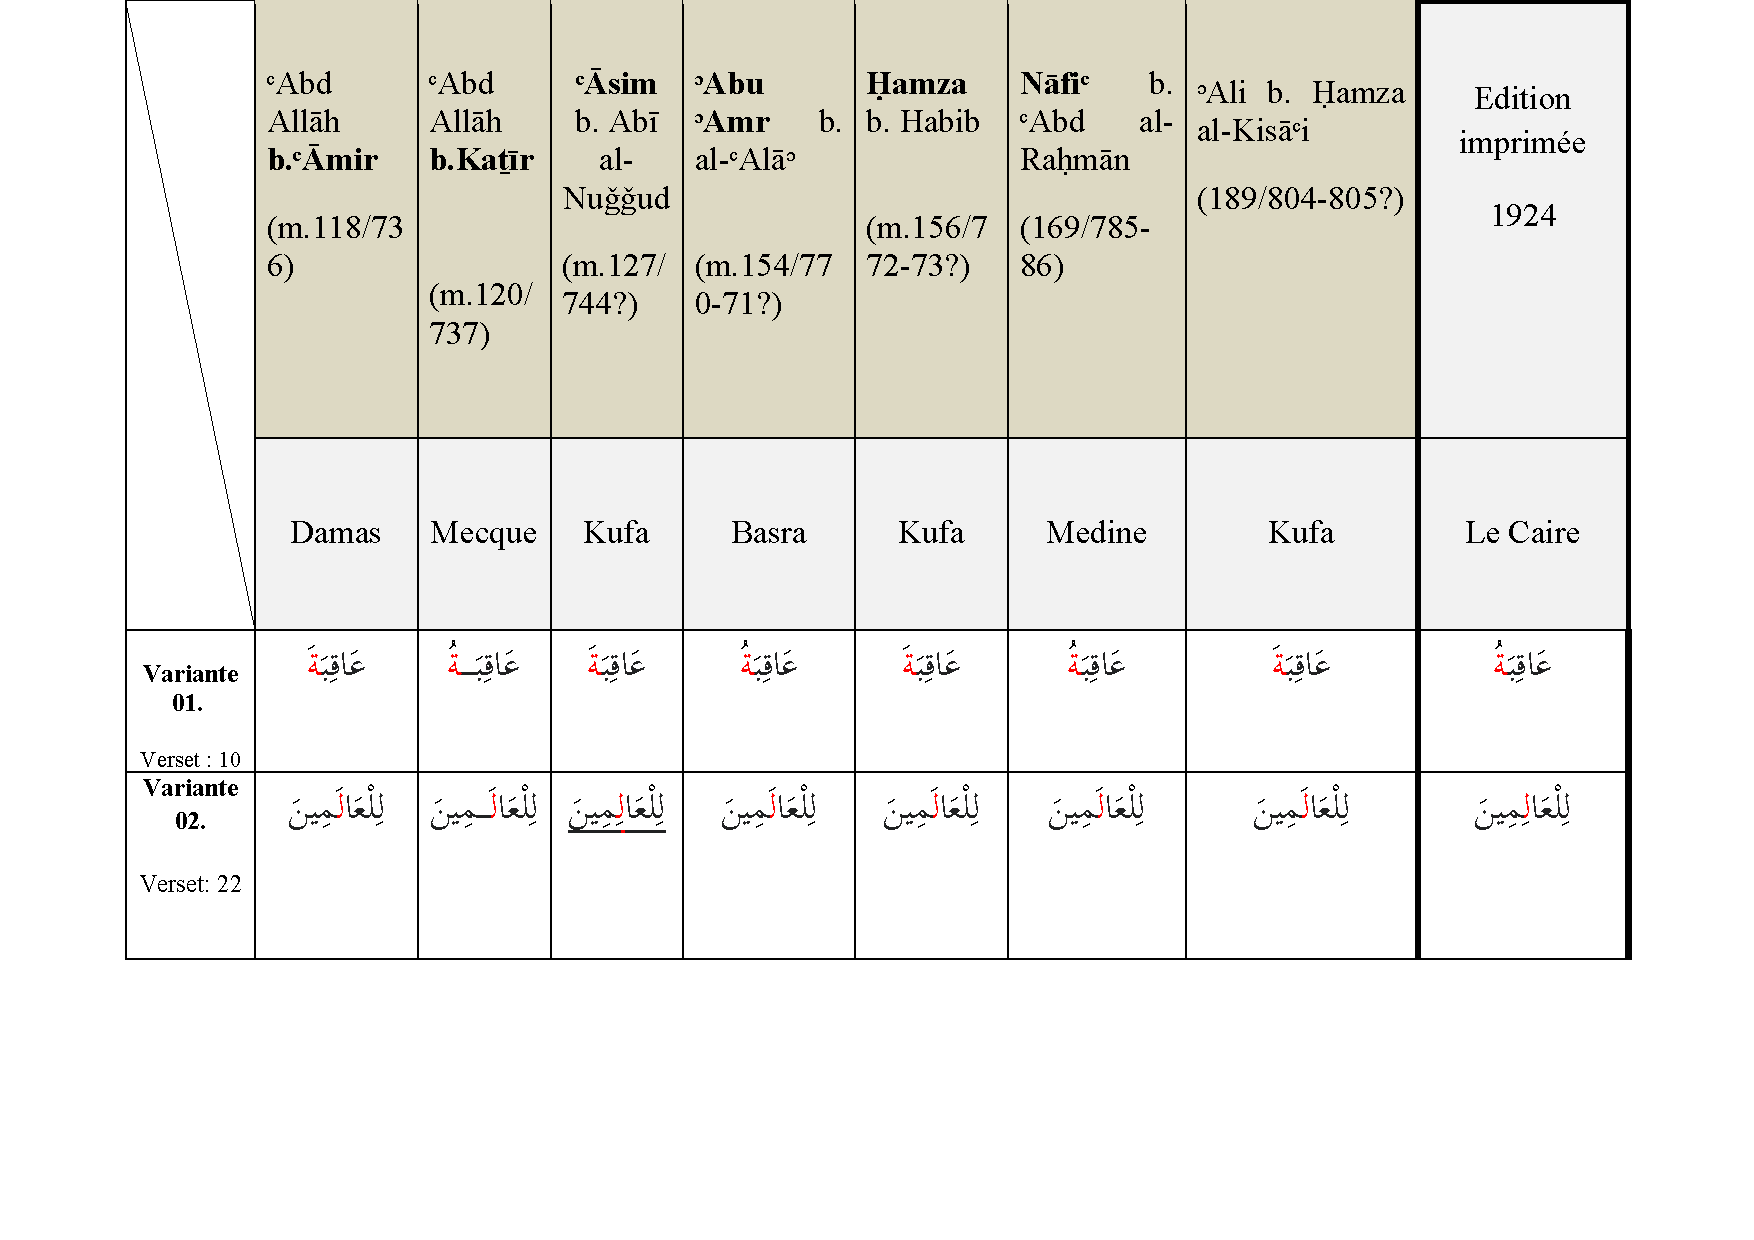
\includepdf[pages=1-3]{table.pdf}










\newpage
\section{	Le deuxième verset de la sourate al-Rūm : Une variante de lecture et deux oublies}

Les six premiers  versets de la sourate 30 rapportent ce qui semble comme un évènement historique.  Le Coran désigne nommément une population :les Romains  ( al-Rūm ) (d'où le titre thématique donné à  la sourate). Si on se base sur le seul contexte des versets  coraniques,  il serai presque impossible de dégager des éléments significatifs pour cette séquence coranique. Ce qui nous  occupe ici n'est pas l'historicité ou non de cet évènement\footnote{ Sur les évènements historiques à cette époque Voir : Mohammed Ali Amir-Moezzi et Guillaume Dye (dir), \textit{Le Coran des historiens}, Paris, les Éditions du Cerf, 2019, vol.II, p. 1073-1075. }, nous nous intéressons à  la façon de lire le deuxième verset. Le sens change notablement selon la manière de lire le verbe  principal de la phrase (le deuxième verbe suit le verbe principal). Chaque lecture assigne une  voix active/passive)  au verbe :  \textit{ġalaba}   ( vaincre ) . Si nous adoptons la lecture  commune et la plus dominante, à la voix passive, nous aurons :             
\begin{Arabic}
    \begin{center}
      \underline{ غُلِبَتِ}  
       ٱلرُّومُ
       ٢
فِيٓ أَدۡنَى ٱلۡأَرۡضِ 
 وَهُم مِّنۢ 
 بَعۡدِ غَلَبِهِمۡ 
 \underline {سَيَغۡلِبُونَ }
٣
    \end{center}
\end{Arabic}
 

\begin{center}
    

\underline{ \textit{Ġulibati}} \textit{al-Rūm fī  ͗adnā al-arḍi wa hūm min baʿdi  ġalabihim} \underline {\textit{sa-yaġlibūna.}}

les Romains \underline{ont été vaincus} dans le pays voisin, et après leur défaite, \underline{ils seront vainqueurs} dans quelques années. 
\end{center}
 
En revanche, si nous adoptons la deuxième façon de lire, à la voix active, nous aurons : 

\begin{Arabic}
    \begin{center}
      \underline{ غَلَبَتِ}   ٱلرُّومُ
٢
فِيٓ أَدۡنَى ٱلۡأَرۡضِ 
 وَهُم مِّنۢ 
 بَعۡدِ غَلَبِهِمۡ 
 \underline {سَيُغۡلَبُونَ }
 ٣
    \end{center}
\end{Arabic}



 \begin{center}
     
 

\underline {\textit{Ġalabati}}\textit{ al-Rūm fī  ͗adnā al-arḍi wa hūm min baʿdi  ġalabihim }\underline {\textit{sa-yuġlabūna}.}

les Romains \underline {ont  vaincu} dans le pays voisin, et après leur victoire, \underline {ils seront vainçu} dans quelques années. 


    
\end{center}

\paragraph{}
L'auteur du commentaire de la sourate al-Rūm  dans   \textit{le Coran des historiens} (le professeur Jan M.F. Van Reeth)  interprète vaguement cette variante de lecture.  Après avoir mentionné les deux façons de lire, voici  ce qu'il est dit:  « C'est cette interprétation du \textit{rasm}, du \textit{ductus consonantique} (ghulibat/sa-yaghlib\=una), qui a été retenue par la majorité des lecteurs et commentateurs musulmans au moyen Age [...] et par les traducteurs modernes »\footnote{Mohammed Ali amir-Moezzi et Guillaume Dye (dir),\textit{ Le Coran des historiens}, \textit{op.cit,} vol. II, p. 1073.} Nous avons trois remarques sur l'interpréation de Jan M.F. Van Reeth :

D'abord, les deux façons de réaliser (ou vocaliser) le premier ou le deuxième verbe du verset ne sont pas  des cas  de \textit{rasm}.\footnote {Si on entend par le terme \textit{rasm} le squelette consonatique dénué de la diacritisation   « \textit{niqāṭ al-iʿǧā}m  »et de vocalisation « \textit{taškīl} »

De nos modestes lectures, le terme \textit{rasm}  (= ductus consonantique, squelette consonantique, \textit{the consonanatal outline} ) est réservé en premier  aux exemplaires des manuscrits coraniques  contenant un squelette consonantique nu } Il s'agit, comme nous venons de dire, d'un cas de flection désinentielle  «\textit{iʿrāb} ». Les deux voyelles (u ET a) du verbe \textit{ġalaba}   ( vaincre ) ont pour fonction principale de fixer une prononciation au verbe et non pas d'indiquer la manière dont il est écrit \textit{rasm}.  

Les cas qui peuvent être interprétés selon le paradigme du \textit{rasm} sont différents. Par exemple dans notre présente édition les variantes numéro : (3, 4, 5, 6? , 7, 9?, 10, 12,13) peuvent être éventuellement interprétées  selon le  \textit{rasm} \footnote{ L'examen minutieux, scientifique et objectif qui peut déboucher sur des résultats et conclusions  nécessite de faire une comparaison entre, 1) d'une part ce que la tradition musulmane entend par Variante de lecture ( les traites de variantes de lectures) car dans plusieurs cas de figure ( voir variante 6 et variante 9) on peut interpréter une variante selon le paradigme philologique ( évolution de la langue) ou selon le paradigme du \textit{rasm} (l'écriture arabe archaïque et évolutions des conventions graphiques) 2) et de l'autre part, un/dès vieux manuscrits coranique(s) de Coran avant les réformes adoptées ( la vocalisation du texte)

D'après nos recherches et dans l'état actuel, nous n'avons pas une typologie ou classification  complète des variantes de lecture  selon des critères scientifiques bien définis. Les études et recherches que nous avons consultés se contentent de  de la recension et de l'aspect descriptif.}

Ensuite, L'auteur du commentaire s'appuie principalement sur ce qu'il lit et comprend ( le sens linguistique immédiat) et  des sources secondaires. Il ne renvoie à aucune source médiévale permettant au lecteur de vérifier si la variante de lecture existe ou non, à partir de quelle époque ?  Enfin, le professeur Jan Van Reeth  rend l'expression \textit{fī  ͗adnā al-arḍi } par : dans le pays voisin ce qui est attesté dans différentes traductions du Coran, mais peu exacte.    \footnote{ Cette traduction est celle de Denise Masson et autres :

Masson Denise,\textit{ Le Coran, introduction, traduction et notes}, Éditions Gallimard, 1967, vol.II, p. 497.  

Et de Hamidullah \url{https://coran12-21.org/fr/sourates/s30} 

Nous pensons que la traduction la plus précise est celle de Regis Blachère. \textit{fī  ͗adnā al-arḍi } = Au confins de notre terre.\url{https://coran12-21.org/fr/sourates/s30}

 L'expression \textit{fī  ͗adnā al-arḍi } ne recouvre  aucune indication  explicite d'un voisinage quelconque ou d'un lieu précis.} 
Nous avons constater lors de la préparation de cette partie de notre recherche que l'une et l'autre  façon de lire\textit{ ġulibati} et \textit{ġalabati} al-Rūm ne sont pas mentionné dans l'édition critique de kitāb al-sabʿa que nous avons consulté, celle établie par Ḍayf Šawq\=i. En toute logique, l'oubli ou (l'erreur) de Ibn Muǧāhid est reprise par son commentateur al-Fāris\=i. Ce dernier ne signale pas cette variante. Toutefois, les deux variantes ont belle et bien existé avant le IVème siècle.   \footnote{ Au moins, jusqu'au /à partir du  fin du IIème siècle les deux variantes de lecture de la sourate al-Rūm ont existé. Voir par exemple:   

Yaḥyā al-Farr\=aʾ (m.207/822),\underline {maʿānī al-qurʾān}, (éd) ʿAlī al-Nadǧār et al \textit{op.cit},  vol.2, p.319.

Abū al-Ḥassan Saʿīd b. Masʿada dit (al-ʾAḫfaš al-Awsaṭ) (m.215/830), \underline{maʿānī al-qurʾān}, (éd) Hudā Qarāʿa, \textit{op.cit}, p. 474.

Nous ignorons si les deux variantes de lecture ont circulé au départ  dans un milieu théologico-dogmatique ou simplement dans un milieu de  spéculations grammaticales.  ( Yaḥyā al-Farr\=aʾ et al-ʾAḫfaš al-Awsaṭ sont surtout des grammairiens et philologues ).  De même, nous n'avons pas consulté des sources après al-F\=aris\=i (le IVème siècle).  Cela mérite une investigation plus profonde. 

Il se peut aussi que les deux variantes existent dans d'autres ouvrages moins connu que\textit{ kitāb al-sabʿa}  de  Ibn Muǧāhid et l'ouvrage de al-F\=aris\=i }



\section{ Variante 1: Cas postposition / cas antéposition}

La première variante de lecture de la sourate al-Rūm est un cas de flection désinentielle 	( \textit{iʿrāb}). En effet, dans le verset 10 de la sourate 30 le mot \textit{ʿāqibata} est lu ou réalisé de deux façons :  
\begin{itemize}


\item   Par la voyelle brève finale « a »  ce qui donne \textit{ʿāqibata}

\item    Par la voyelle brève finale « u »  ce qui donne \textit{ʿāqibatu}
\end{itemize}
\paragraph{}

Ce changement \textit{ʿāqibata}/\textit{ʿāqibatu} est considéré et perçu par la tradition théologique musulmane comme une variante de lecture. Il faut préciser  que cette première variante  n'est pas un cas de  \textit{rasm} ,  mais plutôt un cas qui relève de la grammaire. 

En toute logique, l'explication  ne  peut être que  syntaxique ou lexicale.  c'est ce que al-F\=aris\=i propose de montrer   dans les  notes explicatives données. 

 Voici d'abord, la  séquence du verset qui nous intéresse : 

 
 \begin{Arabic}
   \begin{center}
      
    


ثُمَّ كَانَ 
\underline { عَٰقِبَةَ}
ٱلَّذِينَ أَسَٰٓـُٔواْ ٱلسُّوٓأَىٰٓ أَن كَذَّبُواْ 

   \end{center}

 \end{Arabic}

\begin{center}
  \textit{  ṯumma kāna \underline {ʾāqibata} al-llaḏīna ʾasāʾū al-ss\=uʾū  ʾan  kaḏḏabū}̄
\end{center}



\begin{Arabic}
   \begin{center}
      

ثُمَّ كَانَ 
\underline {عَٰقِبَةُ}
ٱلَّذِينَ أَسَٰٓـُٔواْ ٱلسُّوٓأَىٰٓ أَن كَذَّبُواْ 

   \end{center}

 \end{Arabic}
 
 \begin{center}
     

\textit{
ṯumma kāna \underline {ʾāqibatu} al-llaḏīna ʾasāʾū al-ss\=uʾū  ʾan kaḏḏabū}̄

  \end{center}
  
\paragraph{}
Voyons d'abord   les deux éléments sur lesquels repose les arguments donnés par al-F\=aris\=i.
 \begin{enumerate}
     \item  Au niveau  syntaxique, il s'agit d'une phrase nominale introduite par  l'opérateur verbal ( \textit{kāna} ).  

     \item  Au niveau sémantique, il remarque qu'il y a une antéposition \textit{taqd\=im},  et une postposition \textit{taʾḫīr} dans les composantes de la phrase. 
 \end{enumerate} 


D'un point de vue syntaxique, il s'agit d'une phrase nominale introduite par  le verbe opérateur ( \textit{kāna} ). Ce dernier fait partie d'une classe d'opérateurs dite  \textit{kāna}  est ses consœurs. Quant à la fonction grammaticale de cette classe de verbes   « Il s'agit de verbes opérateurs, ayant pour opérande une phrase nominale, sur laquelle ils ont le même effet syntaxique: il maintiennent le \textit{mubtadaʾ}  au nominatif (alors appelé \textit{ism kāna} et font passer le \textit{ḫabar} à l'accusatif (alors appelé \textit{ḫabar kāna)}. Il est dit \textit{fī maḥal al-naṣb} ( distributionnellement accusatif ). » \footnote{ Pour plus de détail voir: Larcher Pierre,\textit{syntaxe de de l'arabe classique}, Aix-en-Provence, Presses Universitaires de Provence, 2017, p.62.

Nous précisons que  le \textit{mubtadaʾ} et le \textit{ḫabar} sont les deux parties d'une phrase nominale arabe.   Trouver une équivalence parfaite   en français est difficile. Comme souligné par Pierre Larher, le\textit{mubtadaʾ} et le \textit{ḫabar} ont été traduit au départ inchoatif/énonciatif, support/apport et récemment par thème/propos. 

Larcher Pierre,\textit{syntaxe de de l'arabe classique, op.cit} p. 15. Nous avons aussi trouvé la traduction sujet/attribut. certains traductions portent des confusions ou des fois un contre sens

Nous adoptons ici  traduction thème/propos}
\paragraph{}
Si on applique strictement  cette règle de la grammaire classique, nous constatons que  \textit{ʿāqibatu} est grammaticalement correcte , la deuxième lecture \textit{ʿāqibata} est incorrecte et agrammaticale. La raison est simple: dans une phrase canonique et exemplaire le nom qui vient juste après l'opérateur \textit{ kāna} (dit \textit{ism kāna}) doit être au nominatif. Comment alors concilier entre les deux façons ? Il fait appel au niveau sémantique.

Au niveau sémantique,  les deux façons de vocaliser le mot \textit{ʿāqibata} ou \textit{ʿāqibatu} pose aussi le problème de l'ordre des deux des éléments qui constituent la phrase, le thème et le propos (le \textit{mubtadaʾ}  et  le \textit{ḫabar}.). Pour l'auteur de \textit{kitāb al-ḥuǧǧa},   il y a une antéposition \textit{taqd\=im},  et une postposition \textit{taʾḫīr}. Pour analyser les éléments qui sont postposés ou antéposé dans la phrase, il  fait  recours à  la notion technique de   \textit{taqdīr} ( littéralement : estimation ). 
\paragraph{}
Le \textit{taqdīr} est un concept opératoire et  procédé explicatif employé par les grammairiens arabes pour  résoudre certains problèmes que le\textit{qiyās} ( l'analogie ) ne permet pas de résoudre. Il s'agit d'un procédé qui relève du langage. Il consiste, selon Henri Fleisch « l’admission̬ d’un̬ sens̬ virtuel̬ sous̬ le̬ sens̬ naturel̬ d’un̬ mot̬ (\textit{le maʿnā}) autrement dit : une supposition. Il ajoute « le taqdīr̬ es̬t l’opposé̬ de̬ la̬ donnée,̬en̬ ce̬ sens̬ que̬ le̬ grammairien suppose, derrière le texte véritable, un autre texte virtuellement existant et virtuellement agissant.» \footnote {Fleisch Henri, \textit{traité de philologie arabe}, vol, Beyrouth, imprimerie catholique, 1961, p. 7. }

Donnons un exemple pour illustrer ce qui vient d'être énoncer à propos de \textit{taqd\=ir}. La formule dite de la \textit{basmala} qui ouvre  113  dès 114 sourate du Coran est un cas typique de \textit{taqd\=ir}


\begin{center}

\ding{230}\textit{Bismi allāhi al-raḥmāni al-raḥīm}

qu'on traduit généralement par 

  \ding{230} ̠̠̠̠̠̠̠Au̠ nom̠ d’Allah̠ le Tout Miséricordieux, le Très Miséricordieux.
    
\end{center}

En tant que phrase de langue arabe, elle n’est ni proprement verbale (absence  de verbe) ni tout à fait nominale (elle commence par un particule \textit{Bi} ( Au ). De plus, elle n’est  ni interrogative, ni conditionnelle, ni exceptive \textit{istit̠nāʾiya}, ni même vocative (\textit{nidāʾ}). Autrement dit, il s’agit d’une phrase qui ne répond pas entièrement aux canons    terminologiques et conceptuels fixés par les grammairiens. Dès lors, comment un peut-on analyser la phrase pour la rendre intelligible ?  il faut dans ce cas  faire intervenir un/des   élément(s) extérieur(s) extra-phrastique ? comment ?  il n’y a que \textit{taqdīr} qui permet d'assigner un sens. 

Ainsi, le grammairien  ajoute par voie de supposition une expression ou formule de commencement comme :  

\begin{center}
    

     \textit{ awalu mā ʾaqul ʾan bismi allāhi al-raḥmāni al-raḥīm} 
     
    		Que nous pouvons traduire  par
      
      En premier, je dis/énonce qu’au nom de Dieu  le Tout Miséricordieux, le Très Miséricordieux. 

\end{center}

Il est clair donc qu’à travers le \textit{taqdīr}  l’expression supposée (     \textit{ awalu mā ʾaqulʾ}) permet aisément au grammairien de surmonter l’ellipse  dans la phrase. Nous avons essayé dans ces quelques paragraphes d’expliciter la notion de \textit{taqdīr}. retenons que  le \textit{taqd\=ir }  relève plus du langage que de la langue dans le sens où le grammairien intervient par l’ajout d’un élément virtuel pour interpréter  les énoncées.  le \textit{taqd\=ir }  s’oppose au donné et  qu’il peut être un verbe, un nom, un pronom ou encore une expression entière selon le contexte. 

voyons comment  al-F\=aris\=i utilise le \textit{taqd\=ir } pour surmonter le problème de l'ordre des constituants grammaticaux de la phrase et ainsi rendre l'une et l'autre lecture correcte.

\begin{enumerate}
    \item    A l'accusatif :   dans ce cas ce qui vient en premier dans la phrase juste après l'opérateur \textit{kā̄na} c'est à dire \textit{āqibata} n'est pas  le thème (le \textit{mubtadaʾ}) mais plutôt le propos antéposé \textit{ḫabar}. 

    le thème est alors postposé, il est  l'une des deux cas suivants :
    
   
    \begin{itemize}
      
\item \textit{al-ss\=uʾū }: les éléments qui constituent la phrase seront par voie \textit{taqd\=ir } dans cet ordre: 


\textit{ṯumma kāna \underline {al-ss\=uʾū }ʾāqibata al-llaḏīna ʾasāʾū} 



\item   \textit{ʾan kaḏḏabū} : les éléments qui constituent la phrase seront par voie \textit{taqd\=ir } dans cet ordre: 

\textit{ṯumma kāna \underline {al-takḏību  }ʾāqibata al-llaḏīna ʾasāʾū}
      
    
    \end{itemize}

    
    \item Au nominatif  :le le thème (le \textit{mubtadaʾ}) est à l'accusatif : dans ce cas le propos \textit{ḫabar},   est l'une des deux cas:

    

\begin{itemize}
    \item \textit{al-ss\=uʾū }: par voie de \textit{taqd\=ir } la phrase devient: 

   \textit{ ṯumma kāna ʾāqibatu al-musīʾi ̄
al-tak ḏīb bi-ayāt allah}


    \item  \textit{ʾan kaḏḏabū} :
\end{itemize}

    
\end{enumerate}


On voit bien que ce qui est en jeu  est vraiment le sens à donner à la phrase. On peut voir la différence en comparant deux  traductions du même verset vers le français, celle de Hamidullah et celle de Regis Blachère. Chaque traducteur essaye d'être  le plus proche possible et refléter fidèlement  les constituants grammaticaux de la phrase \footnote {\url{ https://coran12-21.org/fr/sourates/s30 } }


\begin{enumerate}
    \item  Puis, mauvaise fut la fin de ceux qui faisaient le mal, ayant traité de mensonges les versets d’Allah et les ayant raillés. (Hamidullah ) 
    \item La fin de ceux qui auront fait le mal sera donc la pire, parce qu’ils auront traité Nos signes de mensonges et qu’ils s’en seront raillés. ( Regis Blachère)
\end{enumerate}

Pour rendre le sens de la phrase les deux traducteurs houent sur l'ordre des éléments de la phrase. 


\newpage
\section{ Variante 12: Cas masculin /cas féminin }

Voici d'abord la variante de lecture 12 de la sourate 30. Nous contentons de la phrase arabe et la translittération. Le sens ne peut pas être visible dans la traduction.   

\begin{Arabic}
\begin{center}

 فَيَوۡمَئِذٖ 
لا
\underline {تَنفَعُ}
ٱلَّذِينَ ظَلَمُواْ مَعۡذِرَتُهُمۡ

\end{center}

\end{Arabic}
\begin{center}
    
\textit {
Fa- yawmaiḏ (in)  \underline {lā tanfaʿu}
allaḏīna ẓalamū 
maʿḏiratuhum  

}
\end{center}



\begin{Arabic}
\begin{center}
فَيَوۡمَئِذٖ 
لا
\underline {يَنفَعُ}
ٱلَّذِينَ ظَلَمُواْ مَعۡذِرَتُهُمۡ

\end{center}

\end{Arabic}
\begin{center}
    

\textit {Fa- yawmaiḏ (in) 
 \underline {lā yanfaʿu}
allaḏīna ẓalamū 
maʿḏiratuhum  
}

\end{center}

La variante de lecture 12 peut être compris selon le paradigme grammatical ou selon le paradigme du \textit{rasm}. 

Si on opte pour  le \textit{rasm}  on a deux cas de figure. 

le premier cas,  l'absence dans un exemplaire coranique de signe particulière sur la première lettre du verbe a donné lieu à cette variante de lecture   \textit{yanfaʿ/
tanfaʿ}.    

le deuxième cas de figure, deux exemplaires coraniques ont donné  lieu à  deux  façons de lire différente \textit{yanfaʿ/
tanfaʿ}. 

La vérification de cette hypothèse  dépasse notre présent travail.
\paragraph{}
Quant au paradigme grammatical, l'interprétation et la compréhension de  cette variante est  radicalement différente.

  Pour le grammairien al-F\=ari\=s  la forme du verbe  \textit{yanfaʿ/ tanfaʿ} est fortement liée  à la suite de la phrase. En effet,  l'une et l'autre façon de lire le verbe  détermine et impose syntaxiquement le genre du  nom \textit{maʿḏiratuhum }  dans la suite de la phrase  . En d'autre mots, il y a une relation d'implication qui donne deux possibilités. Chaque possibilité se base sur une supposition.

\begin{enumerate}

    \item   La première  possibilité: L'élément supposé est le pronom personnel  féminin \textit{hiya} (elle). 
 
 Féminin \textit { tanfaʿ} + féminin  \textit{maʿḏiratuhum }     
 
\item  La deuxième possibilité: L'élément supposé est le pronom personnel  masculin  \textit{huwa} (il). 
 
 Masculin   \textit{yanfaʿ}  +  féminin  \textit{maʿḏiratuhum }.

 \end{enumerate}
 
 

Dans la langue d'aujourd'hui  le genre des mots est bien stable . Un mot comme \textit{maʿḏiratu } mentionné dans le verset est féminin. En revanche, dans la langue arabe classique une telle distinction ( masculin et féminin  ) n'est pas si simple. Plusieurs traités ont été rédigés  au III et IV siècle pour établir des critères de distinction entre les mots féminins et et les mots masculins.   


Par-delà la distinction du genre basée sur le critère de sexe mâle/femelle  une autre distinction de genre concerne non pas l’essence des êtres mais les noms qui expriment des idées, des choses…etc qui n’ont pas de sexe. 

 Les grammairiens  de langue arabes distinguent entre : 
 
\begin{itemize}
    \item Les signes de féminisation: comme le la \textit{tāʾ} finale pour les mots. Mais les signes ne sont pas des critères absolus car  des noms peuvent être féminin  sans avoir de signes particulières.
    
    
    \item  L'absence de signe de féminisation:  il ya  Les noms féminins par  convention et usage  ( \textit{mā yurwā riwayatan} )  dit aussi \textit{ muʾanat̠ sam\=aʿ\=i}  ( le féminin auditif ) c'est à dire des noms féminins qui se sont transmis par voie d’audition et d’usage commun  comme étant  féminin sans  signe spécifique. 
\end{itemize}

Si on applique les règles de la grammaire  on peut dire que la première façon de lire     \textit {Fa- yawmaiḏ (in)  \underline {lā tanfaʿu} allaḏīna ẓalamū 
maʿḏiratuhum  } est  grammaticalement correcte. La deuxième façon est est agrammaticale. Pour al-F\=aris\=i les deux façons sont correctes.  

On peut conclure que  al-F\=aris\=i  donne des explications très diverses selon le cas. Dans quelques c'est le niveau  syntaxique dans d'autres cas c'est le niveau  sémantique. La prise en compte de tous les aspects nécessite une connaissance approfondie  de la grammaire arabe jusqu'à l'époque d' al-F\=aris\=i. Nous remarquons surtout que le défi pour les grammairiens qui ont rédigé des ouvrages sur le Coran est d'apporter des arguments de tout ordre : philologiques, grammaticales, interprétation personnelle, ...etc.   














\chapter{	La transmission, la diffusion  et la réception de \textit{Kitāb al-ḥuǧǧa} : essai de reconstruction  critique  }



\textgoth{L}’édition critique et le commentaire de la \textit{sourate} étaient l’objectif principal de la présente étude. Au cours de la réalisation de notre travail d’édition, un certain nombre d’éléments  qui ne font pas partie du contenu intellectuel de l'œuvre ont retenu notre attention. En effet, par delà les colophons, les lieux d’accomplissement de travail de copie…etc qui attestent d’une identité physique  d'un manuscrit, les annotation( de toute sorte) consignées sur manuscrit témoignent d'une histoire particulière : histoire de transmission, histoire de réception et histoire de diffusion. Les quatre manuscrits de cette étude sont différents. Ils n'ont pas eu  la même histoire. 
Comment rendre cette  histoire visible ? comment devons-nous comprendre la richesse éléments péri-textuels d'un manuscrit et, en même temps, rendre cette richesse analysable et exploitable ? Ces  deux questions principales  nous ont guidé dans cette partie de notre travail.

Comme on peut le constater dans la partie édition ci-joint les élément péri-textuels édités sont seulement  ceux du manuscrit [M]. Nous en avons  trois types: les certificats de lecture-audition \textit{Samāʿ}, les notes de possession et les licence de transmission \textit{iǧāza}.  

\paragraph{}    
Pour le chercheur en études historique ou littéraires, l’analyse des éléments péri-textuels offre plusieurs avantages. D'une part, il constitue  une sorte de mesure du succès des œuvres médiévales et  de l’enthousiasme  soulevée auprès des milieux de réception. Un ouvrage commenté, glosé ou qui a fait l’objet d'enseignements  ne ressemble certainement pas à un autre manuscrit. D'une façon globale, le fait de commenter ou de faire des gloses sur MS ou délivrer des licences de transmission \textit{iǧāza}...etc. L'activité de commentaire  témoigne de la bonne réception et de la dynamique du savoir  De l’autre part, l’intérêt de tels  éléments est historique et documentaire dans la mesure où elles permettent de raffiner notre connaissance historique sur manuscrit une œuvre particulière, un auteur, une aire géographique ou linguistique donnée. 

Pour Gérard Lecomte  l’importance  des certificats d’audition  pour le chercheur  est qu’ils sont : 

« de nature à fournir des renseignements de premier ordre sur des aspects de la vie intellectuelle, religieuse, voire sociale et politique d’un milieux donné à une date donné, et souvent ils s’étendent sur plusieurs générations. C’est bien là que nous entrons en contact avec les transmetteurs, scripteurs et auditeurs, c’est-à-dire avec toute la population studieuse et passionnée des madrasa-s, et que nous trouvons une foule d’indications […] sur tous ses personnages et leurs activités. Bref, c’est bien là une matière historique vivante […]  où les notations austères voisinent avec des traités de mœurs. »\footnote{Lecomte Gérard, \textit{à propos de la résurgence des ouvrages d’Ibn Qutayba sur le ḥadīt}, Bulletin d’Études Orientales (BEO), XXI, 1968, introd. Cité dans : Vajda Géorges, \textit{la transmission du savoir en Islam (VIIe-XVIIIe siècles)}, édité par Nicole Cottart, London, Variorum Reprints, 1983, p. 2.}

Une autre importance des  éléments péri-textuels  est qu’ils permettent de mieux appréhender certains aspects  dynamiques mais, difficilement accessible  par la simple lecture des textes historiques ou littéraires. En outre, ceci nous fournit des renseignements  tel que :  les ouvrages les plus étudiés et la constitution des enseignements et par delà: l'organisation des doctrines et écoles de pensée, les acteurs de la vie religieuse et intellectuelle...etc 

 Malgré leurs importance les élément péri-textuels des manuscrits n'attirent pas beaucoup l'attention des chercheurs contemporains. Nous avons constaté aussi que même les éditeurs des manuscrits  aujourd'hui ignorent complètement ou presque la valeur historique de ces éléments. 
 
 Pour la préparation de cette partie  nous nous sommes appuyé essentiellement sur trois auteurs. 
 
\begin{itemize} 
\item	Un fin connaisseur des manuscrits arabe al-Munǧid Salāh al-Dīn  (1920-2010).  Dans article pionnier\textit{ Iǧāzāt al ͗samāʿ   fī al-maḫ̬ṭūṭātal-qadīma},  il  a dressé une typologie de la majorité des  les composante d'  un  certificat d’audition.\footnote{al-Munǧid Salāh al-Dīn, « Iǧāzāt al ͗samāʿ   fī al-maḫ̬ṭūṭātal-qadīma», in : \textit{maǧalat maʿhad al-maḫ̬ṭūṭāt al-͑ʿarabiya}, le Caire, Vol 1,  1955, pp. 232,251.}. 

Nous avons réadapter le contenu de l'article aux objectifs de cette étude. 


\item	  Dans le domaine francophone, le professeur  Vajda Georges (1908-1981)  a consacré une grande partie de ces travaux à l’analyse des éléments péri-textuel de toute sorte. L'ensemble de ces articles ont été réunis et édités en 1983 sous le titre :  \footnote{Vajda Georges,\textit{La transmission du savoir en Islam (VIIe-XVIIIe siècles)},édité par Nicole Cottart, Londres, Variorum Reprints, 1983.}


\item 	Les deux volumes d’une étude  pionnière et unique dans son genre  \textit{Muʿǧam al- Samāʿāt al-Dimašqiyya,} connu, aussi, par le titre français : les certificats d’audition à Dama 550-750 h./155-1349 Yāsīn Muḥammad al-Sawwās, Muʾmūn al-Ṣāġarǧī̄. Il s'agit d'un index analytique basé sur le déchirement et l'analyse   d'environs 1350 certificats d'audition de la bibliothèque al-Ẓāhiriyya à Damas ( connu aujourd'hui par Maktabat al-ʾAssad al-waṭaniyya). Cet ouvrage nous a aidé surtout pour les noms de personnes.\footnote{Stéfan Leder et al, \underline{Muʿǧam al- Samāʿāt al-Dimašqiyya  al-muntaḫaba 550-750h/1135-1344,} Damas, Institut français d’études arabes à Damas, 1996.}

\end{itemize}




Comme on peut le constater dans la partie édition  les éléments péri textuels sont très divers. Après l'édition, nous avons estimé que l’analyse et le commentaire de ces éléments doit passer inévitablement par une grille analytique qui tient compte de l’ensemble. Nous avons donc  amorcer  la réflexion autour de trois  concepts clés :  

la transmission : comment Kitāb al-Huǧǧa a été transmis d'une génération à une autre ?)  

la diffusion : l’exploitation effective de  Kitāb al-Huǧǧa. c'est à dire les modalités et personnes qui ont contribué à la mise en circulation de l'œuvre.

la réception : Comment l'œuvre a été reçue ?  et dans quel milieu ? est ce que l'œuvre a siccité  d'autres travaux  sur les variantes de lecture ? 


\section{La trans-mission du \textit{Kitāb  al-Huǧǧa} selon le  témoignage du manuscrit [M] }


\subsection{	Les données et informations dégagées des   certificats de lecture-audition ( \textit{samā}ʿ)  }


Comme nous pouvons le constater dans la partie édition, nous avons deux  types de certificats de lecture-audition :  collectif et individuel. Pour chaque type nous avons quatre certificats, ce qui fait huit certificats en total. Les  quatre certificats de lecture audition collectif  ont été consignés sur  la page de fin de chaque volume \textit{ǧuzʾ}.  En revanche, les certificats de lecture-audition individuels  figurent sur la page de titre de chaque volume \textit{ǧuzʾ}.  

\paragraph{}
D'une façon générale,  L'un et l'autre type sert à un objectif et une finalité précise.   les certificats individuels ont pour objectif principal de donner une autorisation à une personne compétente pour  transmettre une œuvre.\footnote{NB : le certificat de lecture individuel dans ce cas vaut une licence de transmission \textit{igāza} Pour plus de détail voir 
 

al-Munǧid Salāh al-Dīn,  \underline{ Iǧāzāt al- ͗samāʿ   fī al-maḫ̬ṭūṭātal-qadīma} \textit{op.cit}, pp.234-238. Et

During, J. et al,« sam\=aʿ,» \textit{ EI2}, Leiden, Brill, (en ligne.) 
} (Kitāb  al-Huǧǧa dans notre cas).  Les certificats  de lecture-audition collectif attestent que des enseignements d'instruction sur le texte coranique ont eu lieu. Vu la richesse et les informations mentionnées dans  les certificats de lecture-audition de notre Ms, nous pouvons même parler des actes de lecture-audition ( des actes notariés dans le langage juridique et notarial d'aujourd'hui)

Les informatisons ci-après ont été tirées des certificats de lecture-audition collectif. Elles reflètent et donnent à voir  une image assez précise sur le déroulement, la composition  des enseignements et la hiérarchie des responsabilités .  

\begin{enumerate}
    \item 	\textbf{L’enseignant et responsable de la tenue des séances de lecture-audition de \textit{kitāb al-ḥuǧǧa} :} Abū al-Yumn Zayd b. al-Ḥasan b. Zayd al-Kindī.  (un seul dans les quarte certificats de lecture-audition.)  Il est désigné par une kyrielle de surnoms, titres de glorification, qualificatifs. Ce qui  nous intéresse ici est le qualificatif technique. (Voir la correspondance dans la partie édition )

\ding{93} certificat de  lecteur- audition collectif,  Vol.1. lig :23 dit,
\textit{al-Šayḫ al-musmiʿ } ( le maître de la lecture-audition )

\ding{93} certificat de  lecteur- audition collectif,  Vol.2. lig :6. dit,
\textit{al-Šayḫ al-musmiʿ } ( le maître de la lecture-audition )

\ding{93} certificat de  lecteur -audition collectif,  Vol.3. lig :  5 et 6. dit,\textit{al-Šayḫ al-musmiʿ } ( le maître de la lecture-audition )

\ding{93}  	 certificat de  lecteur- audition collectif,  Vol.4. lig :28 dit,\textit{al-Šayḫ al-musmiʿ } ( le maître de la lecture-audition )


    
\item \textbf{ Le lieu :} La ville de Damas dite \textit{al-maḥrus}a ( la bien gardée ) \footnote   { Hors le cadre de ce mémoire, d'après nos lectures il semble que ce qualificatif et titre :  \textit{al-maḥrusa} ( la bien gardée ) est disputé entre plusieurs villes et capitales dans le monde: Alger, le Caire, Tripoli. 

Des villes européennes aussi: 
Paris est surnommée aussi \textit{al-maḥrusa} ( la bien gardée ) dans l'éditon de  kitāb de Sibawayh par Hartwig Derenbourg en 1881.

Leiden au pays-bas  et Uppsala au Suède , ont été surnommée de la méme façon dans l'éditon de \underline {al-kāmil fi al-tārīḫ } de Ibn al- ʾAṯīr par  Carlos Johannes Tornberg entre 1851-1867.  }, plus précisément à  l’école al-ʿAzīziyya.\footnote{ Pour les écoles  à Damas voir: ʿAbd al-Qādar b. Moḥamed al-Naʿīmī, \underline {al-dā̄ris fī tārīḫ al-madāris}, (éd) Ibrāhīm šams al-Dīn, Beyrouth, Dār al-kutub al-ʿilmiya, 1990.  } 


\item 	\textbf{La date :} selon le volume : 
\begin{itemize}
    \item •	\textbf{Dans le premier volume :} La dernière séance a eu lieu au mois de (Ḏī al-Ḥiǧǧa) l’année hégirienne   606. Ce qui correspond au mois de mai 1210.


\item•	\textbf{Dans le deuxième volume }: même période que le premier volume.

\item•	\textbf{Dans le troisième volume :} La dernière séance s'est tenue au début  \textit{mustahal}  du mois de \textit{safar} (le deuxième mois de l'année hégirienne ) de l'an   607. Ce qui correspond au mois de juillet de l’an  1210.  
\item•	\textbf{Dans le quatrième et dernier volume :} La dernière séance de la lecture-audition de ce volume s’est tenue le dimanche, 12 du mois de\textit{ safar}  (le deuxième de l’année hégirienne) de l'an 607. Ce qui équivaut au jeudi 4 aout de l’an 1210.     
\end{itemize}

\item \textbf{Durée totale des séances de lecture-audition :} 
De la fin de la lecture-audition du premier volume ( le dernier mois de l'an 606/mai 1210) jusqu'à la fin de la lecture -audition du dernier volume  nous avons presque deux mois et demi chevauchant entre deux ans de l'hégire: 606 et 607. 




\item \textbf{Le possesseur de la copie sur laquelle porte la lecteur : } il s'agit de:  
Muntaǧab al-Dīn  Muntaǧab b. ab\=u al-ʿizz b. al-Rašīd al-Hamaḏ̠ānī.
Il est désigné par des qualificatifs légèrement différents. 

\ding{93} certificat de  lecteur- audition collectif,  Vol.1. lig : 8. \textit{ṣāḥib al- kitāb}  le possesseur du livre 


\ding{93} certificat de  lecteur- audition collectif,  Vol.2. lig : 7. 
\textit{al-nusḫa lahu}  la copie [de lecture] lui appartient 


\ding{93} certificat de  lecteur- audition collectif,  Vol.3. lig : 7. \textit{ṣāḥib al- kitāb}  le possesseur du livre )


\ding{93} certificat de  lecteur- audition collectif,  Vol.4. lig : 6 et 7. \textit{ṣāḥib al- kitāb}  le possesseur du livre 



\item \textbf{La deuxième copie de lecture:}  En plus de la copie de   la lecture collective, celle de  Muntaǧab al-Dīn  Muntaǧab b. aby al-ʿizz b. al-Rašīd al-Hamaḏ̠ānī,
 une deuxième copie  sert, à ne pas en douter,  pour les corrections et les constats du maître.  Cette dernière est désignée dans les quatre certificats comme un  \textit{aṣl al-šayḫ} ( l' original du maître )  voir :
 
 \ding{93} certificat de  lecteur- audition collectif,  Vol.1. lig : 23
 
\ding{93} certificat de  lecteur- audition collectif,  Vol.2. lig : 26

\ding{93} certificat de  lecteur -audition collectif,  Vol.3. lig : 21

\ding{93}  	certificat de  lecteur- audition collectif,  Vol.4. lig : 28




\item \textbf{Le lecteur du livre :} la personne qui a lu  à haute voix sans aucun doute   \textit{ kitāb al-ḥuǧǧa } devant le \textit{Al-Šayḫ al-musmiʿ }  le maître de la lecture-audition  durant  toutes les séances est : 
Šihāb al-Dīn aby Isḥāq Ibrāhīm b. Moḥamed b. aby Bakr al- ʿAfṣī. Voir


\ding{93} certificat de  lecteur- audition collectif,  Vol.1. lig : 3 et 4.

\ding{93} certificat de  lecteur- audition collectif,  Vol.2. lig : 3 et 4.

\ding{93} certificat de  lecteur- audition collectif,  Vol.3. lig : 3.

\ding{93} certificat de  lecteur- audition collectif,  Vol.4. lig : 3.

\item \textbf{Le greffier/scripteur des certificats de lecture-audition:} Les quatre certificats de lecture-audition ont été consignés par écrit par :
ʿAbd al-Ǧalīl b. ʿAbd al-Gabbār ʿAbd al-Wāsiʿ al-Abharī. Il est désigné par deux qualificatifs   légèrement différents.


\ding{93} certificat de  lecteur- audition collectif,  Vol.1. lig : 22. pas de qualificatif.

\ding{93} certificat de  lecteur- audition collectif,  Vol.2. lig : 25 \textit{muṯbit/muṯabit al-asmā ̄ʿ} ( celui qui a fixé/transcrit les noms )

\ding{93} certificat de  lecteur -audition collectif,  Vol.3. lig : 20 dit :  \textit{muṯbit/muṯabit asmāʾihim} ( celui qui a fixé/transcrit leurs noms )

\ding{93}  	certificat  de  lecteur- audition collectif,  Vol.4. lig : 27 dit : \textit{Kātib al-samā ʿ} ( le scripteur de l’acte de lecture-audition )


\item \textbf{Le nombre d’auditeurs:} Il varie sensiblement entre les quatre certificats.

Si on fait abstraction de ce que nous n'avons pas réussi à lire, on peut dire qu'une séance de lecture-audition compte environ 60 personne (vol.2). 
( On a utilisé la conjonction de coordination  \textit{wa} ( et ) pour compter et séparer les différentes composantes d'un seul nom propre. ( voir la suite du travail )  

\item \textbf{ La qualité des auditeurs :}  il y a surtout des juges, juges suprême, savant religieux, savant, imam, \textit{naq\=ib} mais, majoritairement des personnes ordinaires.   
\item \textbf{ Le genre et classe d'âge des auditeurs:}
l s'agit d'un publique  adulte  et masculin. quelques uns sont liés par des liens familiaux ( fils, cousin...etc) 
\item \textbf{Le suivi des enseignements et l’assiduité :} entre le premier et dernier autant de noms disparaissent ou réapparaissent.   

\item \textbf{Titres honorifiques :} il s'agit surtout de divers qualificatifs et titres pour le maître. Il s'agit de qualificatifs et titres à connotation religieuse  ou intellectuelle  :

\ding{93} \textit{Šayḫ al-islām} : ( littéralement : Le maître de l'islam) mais, il s'agit  généralement d'un titre officiel  \footnote{Pour plus de détail voir la notice de  \textit{S̲h̲ayk̲h̲ al- Islām}  dans:
  
Kramers et al,  « S̲h̲ayk̲h̲ al-Islām,»\textit{ EI2}, Leiden, Brill, en ligne.} 

\ding{93} \textit {tāǧ al-dīn} : ( littéralement: la couronne de la religion (sous-entend la religion islamique) ) 

\ding{93} \textit{ʿalāmat al-zamān}: le plus connaisseur de son temps 


\ding{93 } \textit{farīd al-dahr} : l'unique de son temps

\ding{93} \textit{al- ʾaǧǧal} : le plus vénéré

\item \textbf{ Modes et termes d’authentification  des séances de lecture-audition} il s'agit de trois modes:


\begin{enumerate}
    \item  Authentification par le scripteur des certificats: les termes employés sont: 

  
\ding{93} certificat de  lecteur- audition collectif,  Vol.1. lig :24

 \ding{50}  \textit{ ṣaḥḥa wa ṯabata/ ṯabuta} : ceci est correcte et fixé. 

\ding{93} certificat de  lecteur- audition collectif,  Vol.2. lig 27

\ding{50}  \textit{wa ṣaḥḥa } : ceci est correcte

\ding{93} certificat de  lecteur -audition collectif,  Vol.3. lig : 21

\ding{50}  \textit{ ṣaḥḥa wa ṯabata/ ṯabuta} : ceci est correcte et et fixé. 

\ding{93} certificat de  lecteur -audition collectif,  Vol.3. Pas d'authentification par le scripteur des certificats. 

\ding{93}  certificat de  lecteur- audition collectif,  Vol.4. lig :28

\ding{50}  \textit{wa ṣaḥḥa }


\item  Authentification par le responsable des enseignements (abū  Zayd al-Kindī.)  à la toute fin de chaque certificat:

\ding{93} certificat de  lecteur- audition collectif,  Vol.1. 

 \ding{50}  Ceci est correcte/valable, rédigé par abū   al-Yumn Kindī. de sa propre main ( \textit{bi-ḫaṭih} ) 

\ding{93} certificat de  lecteur- audition collectif,  Vol.2. 

 \ding{50}  Ceci est correcte/valable, rédigé par abū   al-Yumn Kindī. de sa propre main ( \textit{bi-ḫaṭih} ) 


\ding{93} certificat de  lecteur- audition collectif,  Vol.3. 

 \ding{50}  Ceci est correcte/valable, rédigé par abū   al-Yumn Kindī. de sa propre main ( \textit{bi-ḫaṭih} ) 

\ding{93} certificat de  lecteur- audition collectif,  Vol.4. 

 \ding{50}  Ceci est correcte/valable, rédigé par Abū   al-yumn Kindī. de sa propre main ( \textit{Bi- ḫaṭih} ) 


\item Authentification  par des termes canoniques de la culture religieuse musulmane : que le bon Dieu soit remercié, prière au prophète Muḥammad ...etc ( voir vol.1 lig: 24 et vol.2 lig: 27)


Il faut noter qu'un exemplaire amputé de ses termes   de glorification de Dieu et de son prophète vaut moins, voire douteux. Ces expressions changent ( dès fois sensiblement)  entre les époques et les géographies et les doctrines. à titre d'exemple:

Dans le cas d’un Ms rédigé, enseigné ou  circulant dans un environnement d’obédience shiite, on peut trouvé ( ce n'est pas absolu) des  glorifications et expressions élogieuses  destinées   au gendre du prophète et dernier calife de l'Islam : ʿAlī ou \textit{ahl al-Bayt}. 

Souvent sous-estimé dans l'édition des manuscrits,  ces expressions  valent , sans aucun doute, aux yeux des destinataires d'un manuscrit. Certains mots déterminent  souvent le destin et la destination d'un manuscrit. Pour le chercheur, ces expressions aident quelques fois à  estimer la date de rédaction d'un manuscrit ou de voir l'évolution du lexique et la la façon de nommer  ( voir nos constats sur le titre  de l'œuvre éditée) ou encore, pour le développement des pratiques  intellectuelles et les  frontières et crispations  entres doctrines  d'une façon  générale.   
\end{enumerate}
\end{enumerate}

    \subsection{ Constats sur la  composition  d'un certificat de lecture-audition et la structure onomastique   }

Après avoir extrait toutes les informations nécessaires, il est aussi important de montrer comment se structure un certificat de lecture-audition. Nous avons une seule et même schéma  dans les quatre  certificats comme suit:   

\ding {42} il a entendu:  

\ding{232} le numéro du volume ( 1,2,3,4) \ding{232} rappel du titre de l'œuvre 
\ding{232} le nom du responsable de lecture-audition \ding{232} par quel voie le l'œuvre est transmise le \textit{sanad} \ding{232} la personne qui lit texte devant l'auditoire \ding{232} les noms les plus prestigieux (juges suprême, savant, ...etc) 
 \ding{232} les noms les moins connus \ding{232} celui qui a transcrit les noms de l'auditoire  \ding{232} la date de la dernière séance \ding{232} le nom de la  ville \ding{232} le nom du lieu exacte \ding{232} l'authentification du responsable des enseignements.

\paragraph{}
La composition des noms propres des certificats de lecture-audition mérite une attention particulière. L'analyse des composantes d'un nom propres nous permet de voir la manière de nommer les personnes au VIIème siècle. D'une manière générale, le mon dans les pays de l'islam à l'époque médiévale   suit un schéma particulier.  Il reflète et met en valeur certains aspects de la culture et de la civilisation musulmane tel: la religion,  les parlants directes  et/ou les ancêtres., les lieux géographiques.. etc.\footnote{ L'importance des noms de personnes est lié aux différentes disciplines de la religion musulmane ( hadith, biographie, ..etc) et le mode de fonctionnement de la société  ( mariage, filiation \textit{nasab},...). A ce titre,  le nom propre a retenu l'attention des auteurs musulmans depuis une longue date. On peut citer :

 l'ouvrage   de  : al-Samaʿānī ʿAbd al-Karīm  (m.562/1166) , \underline {al-ʾAnsāb}, (éd) ʿAbd al-Raḥmān al-Yamānī et al, Haydar Bād, Dāʾirat al-mʿārif al-ʿuṯmāniyya, 1er éd, 1962.    

ou les ouvrages consacrés à la critique des traditionalistes et transmetteurs. connus par: 
\textit{ʿilm al-riǧāl} ( littéralement :  la sciences des hommes )   ou  \textit{ʿilm al-ǧarḥ wa al-taʿdīl }} 


Dans notre  édition, un nom propre est long,  très long même. Dès fois, il fait une  chaîne onomastique  d'une ligne ou  une ligne et demi, ce qui ne permet pas souvent de savoir qui est qui ou qui est le fils de qui ? 

Cependant si on a certains notions théoriques sur la façon de nommer comme le   \textit{Laqab}  la\textit{Kunya}...etc la tache devient moins difficile. 

 Jacqueline Sublet a consacré une grand part de ses travaux aux noms propres dans les pays musulmans. Nous adoptons  ici les définitions qu'elle a donnée.\footnote{Sublet Jacqueline, \textit{Le voile du nom essai sur le nom propre arabe,} Paris, PUF, 1990. pp. 9-11.}  

 \ding{182} Le \textit{ism} ou \textit{ism ʿalam}: nom reçu à la naissance, souvent traduit en français   par « prénom  à tort puisque on a pas ici la séquence prénom suivi du nom de famille [...] Accompagné des \textit{ʾism} du père et des ancêtres, il forme la généalogie \textit{nasab} patrilinéaire à de très rares exceptions près ( par exemple: 	Aḥmed fils de Moḥammad  fils d’Aḥmed...etc

  \ding{183} La \textit{kunya} un élement composé avec « Abū»  au masculin « Umm » au féminin  deux termes qui signifient père et mère, mais aussi    «possesseur de »
« Abū» « Umm »   «qui a » et leurs équivalents ( par exemple :  Abū ʿAli = le père de Ali,   Umm Ḥassan= la mère d Ḥassan [...] Le mot \textit{kunya} est intraduisible car il s'agit, on le verra, d'un élément dans le contenu est complexe. La \textit{kunya}, porté en principe  par des musulmans libres, est soit reçu à la naissance, soit acquise par l'esclave affranchi.

   \ding{184} Le \textit{laqab}: surnom, titre, titulature ou encore surnom conventionel  dont les plus connus sont composés avec al-dīn en référence à la « religion musulmane », « la fois » ( par exemple : Šihāb al-dīn […] est reçu à la naissance ou acquis. [...] chaque individu est susceptible d'avoir plusieurs de ces  surnoms dont l'un  peut être le nom sous lequel il est le plus connu \textit{šuhra }

 \ding{185}  La \textit{nisba} adjectif terminé par ī \footnote{Voir les exmples de \textit{nisba} qui viennent juste après. } (i long) \textit{iyya} au féminin ou \textit{ānī} marque la connexion du personnage avec une idée, un lieu, un évènement, un individu notamment. Exemple de notre édition : al-ʾAnmāṭī=  le vendeur de tapis\footnote{ al-Samaʿānī ʿAbd al-Karīm, \underline {al-ʾAnsāb}, \textit{op.cit,} p. 378.} 

Les noms des certificats de lecture-audition de notre édition sont de deux sortes soit une structure complète contenant toutes les composantes que nous venons de citer : La \textit{kunya},  Le \textit{laqab} ...etc soit une structure abrégée et minimale de quelques composantes.    

Voici deux exemples  illustratifs:

\begin{enumerate}
 

\item La structure complète:   \textit{laqab} \ding{224} \textit {kunya}    \ding{224} \textit {ism}  + nom du père + nom d'un ancêtre    \ding{224} \textit{nisba }

Ex: šayḫ  al-islām Abū al-Yumn Zayd b. al-Ḥasan b. Zayd al-Kindī. ( Voir la partie édition: Vol.2 lig.2)

\item La structure abrégée :   \textit{kunya} \ding{224} \textit  \textit {ism}  ( vol.2. lig :12) 

Ex:
Abū al-Ḥasan ʿAbd al-Wahāb

\end{enumerate}
  




\begin{multicols} {2}
\begin{itemize}
    

    

    


\item al-Kindī=  La ville  historique de Kinda (le Yemen actuel)

\item al-ʾĀmidī=  La ville kurde de ʾĀmid ( la Turquie actuelle)  

\item al-Saḫāwī= la ville de Saḫā  ( l'Egypte actuelle)

\item al-ʾAsfahānī= Ispahan ( l'ancienne perse et l'Iran actuelle)

\item al-Hamaḏānī=  la ville de Hamaḏān  (en Iran actuel) 

\item al-Ḥalabī= Ḥaleb/Alep   ( la Syrie  actuelle) 

\item al-Tanuḫī=  En référence à une tribu arabe

\item al-Ḫazragī=  En référence à une tribu arabe

\item al-Turkī= le turque

\item al-ʿAsqalānī=  la ville de ʾAsqalān   (en Palestine actuelle)


\item al- Ḏarīr= l'infirme

\item al-Baʿlabakī= la ville de  Baʿlabak  (en Liban actuel) 

\item al-Dimašqī= la capitale  historique  (la Syrie actuelle)

\item al-Wasiṭī= la ville historique  fondée par Al-Haǧǧāǧ b. Yusuf. ( en Iraq actuel) 

\item al-ʾAbharī=  La ville historique  de ʾAbhar (en Iran atuel)



 \end{multicols}

\begin{center}
\textbf{    Exemples de noms de relation \textit{nisba} tirés des certificats de lecture-audition édités}

\end{itemize}




  
 

\newpage
\normalsize
\subsection{Abū Zayd al-Kindī :  un grammairien,  spécialiste de varianets de lecture  et chef d’une \textit{mašyaḫ̬a} ( un cercle d’enseignement religieux)}

L’édition des certificats de lecture-audition   nous a montré un personnage clé et central  dans la longue histoire d'un manuscrit de\textit{ kitāb al-Ḥuǧǧa }: Abū al-Yumn al-Kindī. Il est un chaînon très important dans la transmission et la diffusion de l’œuvre de al-Fārisī en Syrie ayyoubide. Bien plus, Abū al-Yumn al-Kindī nous fournit quelques renseignements  très instructifs sur la trajectoire  traversée par cette œuvre.     
\paragraph{}
Abū al-Yumn al-Kindī 520/1125-613/1216 est un personnage bien connu de la littérature biographique du VIIème siècle et les siècles suivants. \footnote{ Entre autres : al-Ḏahabī Šams al-Dīn, \underline  { Siyar ʾaʿlām al-nubalā}ʾ,(éd) Šuʿayb al-ʾArnaʾuṭ, \textit{op.cit}, vol.22, p.34}. 
D'après  al-Ḏahabī son nom complet est : Tāǧ al-dīn abū al-Yemn Zayd b. al.Hasan b. Zayd b. al-Ḥasan b. Zayd b. al-Ḥasan 
 b. Saʿīd b. ʿIṣma b. Ḥimyar al-Kindī al-Baġdādī le lecteur (du Coran) le grammairien, le lexicologue, le hanafite ( la doctrine hanafite) ̄. Il a fait ses études à sa ville natale Bagdad
 et Hamaḏān. Il a finit par s'installer en Syrie ( Šām) pour se consacrer à l'enseignement de la grammaire et des variantes de lectures jusqu'à sa mort.
\paragraph{}
 Toutes les sources et études consultées soulignent le rôle imminent de abū al-Yumn al-Kindī 
 dans les dynamiques de la vie religieuse et intellectuelle à Damas. Il fut  surtout le chef d'un un cercle d’enseignement religieux ou ce qu'on appelle dans la littérature spécialisée la \textit{mašyaḫ̬a}\footnote{ Terme technique forgé du nom \textit{Šayḫ} c'est à dire un chef   dans le sens spirituel et intellectuel}. Deux exemples peuvent illustrer la place et le statut de Abū al-Yumn al-Kindi à la fin du VI et le début du VIIème siècle. 

 Dans son étude sur la ville de Damas   Louis Pouzet  note  ainsi la richesse de la bibliothèque de al-Kind\=i 

« Ce n'est pas un hasard si, dans l'inventaire de la bibliothèque de Abū al-Yumn al-Kindi, ̄mort en 613/1217 à Damas, et dont  nous avons parlé plus haut, « sciences du Coran»    (\textit{ʿUlūm al-Qurʾān} ) sont placées en tête de liste avec 140 volumes sur un total de 761, précédées immédiatement en nombre par les sciences  grammaticales (\textit{ ʿUlm al-naḥw wa al-taṣrīf}) avec 175 volumes...  »

Dans son travail sur les voies de transmission des copies manuscrites de \textit{Kitāb} de S\=ibawayh, Geneviève Humbert souligne aussi le rôle important de Abū al-Yumn al-Kindī  dans les trajectoires de transmission de \textit{Kitāb}  de S\=ibawayh. 
« l'existence d'une recension ou du moins d'une influence d'Abū al-Yumn al-Kindī dans la transmission de \textit{Kit\=ab} au VII/XIIIe siècle est attestée par deux autres copies : la copie 2Ç ( dont le complément de fin a été ajouté par un copiste qui cite quelques une des questions  qui lui sont adressées), et la copie 2G ( le Kit\=ab est lu dans la mosquée des Omeyyades, à Damas, devant lui).» \footnote{Humbert Geneviève, \textit{les voies de transmission de kitāb de sībawayhi}, Leiden, Brill, 1995, p. 353.}

\section{La  diffusion du \textit{Kitāb  al-Huǧǧa} selon le  témoignage du manuscrit [M] }
\subsection{Une chaîne  de transmission ( \textit{isnād} )  ascendante et ininterrompue}



Par le procédé de transmission dit ( \textit{isnād} ) le contenu intellectuel du   Kitāb al-Huǧǧa se rapporte, par une longue chaîne de transmetteurs ( \textit{ruwāt} ), jusqu’à son auteur: abū ʿAlī al-Fārisī. Cette chaîne de transmetteurs est, à la fois, ininterrompue et ascendante. C’est-à-dire qu’elle part du transmetteur le plus récent  jusqu’au  l'auteur  qui a rédigé/dicté le contenu intellectuel du livre. Plus concrètement, la chaîne  remonte  dans le temps et l’espace d’un XII siècle damascèn  jusqu’à IV siècle à Bagdad, soit environs deux siècles et demi  et quatre générations  qui auraient transmis ou étudié le livre. En d’autres mots, cela va du   abū Zayd al-Kindī  (m.613)  pour arriver , finalement, jusqu’à  Abū ʿAli al-Fārisī (m. 377).  
\paragraph{}
Avant tout nous rappelons  que  le terme technique  \textit{isnād}, littéralement  veut dire ( support ) est un procédé de transmission de faits, des propos…etc .  En gros, le \textit{isnād} consiste  à faire recours à une liste transmetteurs (des personnes physiques) qui se succèdent  (ou pas)  dans le temps chronologique et, qui ont pour fonction d’être des garants de l’authenticité de tel ou tel information rapportée. 
Transmettre par la voie du  \textit{isnād} a vu le jour vers le  deuxième et troisième siècle de l’hégire principalement dans le sillage de  la collection, la critique et la canonisation des traditions orales attribuées au prophète de l’slam « hadith-s ». Ce procédé de transmission fut d’abord oral, il devient à partir du quatrième et cinquième siècle, sous l’effet de l’élargissement de l’enseignement de la religion, de plus en plus authentifié par écrit.\footnote {Il est pratiquement impossible de rappeler ici l’évolution historique, les retombés socio-politiques et les codes terminologiques  du \textit{isan̄d} et du hadith. Nous renvoyons vers les notices suivantes dans l’encyclopédie de l’Islam EI2 : \textit{isnād, sanad, riwaya}.}


\subsection{Quatre  chaînons et trois générations de transmetteurs} 

Comme nous pouvons lire dans la partie édition. ; abū Zayd al-Kindī  déclare qu’il a lu/entendu \footnote{ l'expression exacte est \textit{aḥad maqrūʾtī}  ( l’un de mes lectures ). Vol. 1. certificat de lecture individuel)

On ne sait  dans quel contexte et par quelle voie cette lecture a été faite  }  le contenu textuel directement  de son maître : l’imām ʾAbū Muḥammad dit
le lecteur du Coran ( \textit{muqriʾ} )et  grammairien . Ce dernier, selon Abū Zayd al-Kindī, tenait le texte  de Abū Ṭāhar b. Siwār dit le lecteur du Coran. Ṭāhar b. Siwār \textit{al-muqriᶜ} , qui lui-même le tenait du Ab\=u ʿAbd allāh al-Āmidī. Ce dernier le tenait, toujours selon le témoignage de Abū Zayd al-Kindī, de al-rabʿi  ̄le grammairien , qui, de son côté, le tenait directement de l’auteur-source Abū ʿAlī al-Fārisī.   


Voyons très brièvement ce que dit la littérature biographique de chaque chaînon 

\ding{202}	\textbf{Le premier chaînon}  	Le premier chaînon  est Abū Muḥamd b. ʾAbd allāh b. ʾAli b. ʾAhmed, dit le lecteur du Coran et  grammairien  né à Bagdad en 453  et mort à  en 541.  Il a également rédigé des ouvrages sur les variantes de lectures coraniques. \footnote {al-Ḏahabī Šams al-Dīn, \underline  { Siyar ʾaʿlām al-nubalā}ʾ,(éd) Šuʿayb al-ʾArnaʾuṭ , Beyrouth, muʾasasat al-Risāla, 1985, vol 20,  pp. 130-131. } 

\ding{203}	\textbf{Le deuxième chaînon}
est Abū Ṭāhar Aḥmad b. ʿAlī b. ʿUbayd allāh  b. ʿUmar b. Siwār, dit, al-Ḥanafī al-Baġdādī  en référence à la doctrine hanafite et à la ville de Bagdad  est né en 412.   C'est est un traditioniste et  lecteur du Coran ( \textit{muqriʾ} ).   Ibn Siwār est mort  en 496.   \footnote {al-Ḏahabī Šams al-Dīn, \underline  { Siyar ʾaʿlām al-nubalā}ʾ,(éd) Šuʿayb al-ʾArnaʾuṭ, \textit{op.cit}, Vol 19, pp. 226-227.}


\ding{204}	\textbf{Le troisième chaînon} al-Ḥusayn b. ʿAlī b. ʿAbd allāh al-Āmidī Abu ʿAbd allāh le grammairien est mort en  466.\footnote {Al-Ṣuyuṭī Ǧalāl al-dīn, \underline {Buġyat al-Wuʿāt}, (éd) Ibrāhīm Abu al-Faḍl, Beyrouth, Al-maktaba al-ʿasriya
Vol, p.536. 
 

Dans la même notice biographique, il est dit que al-Āmidī Abu ʿAbd allāh fut l'un des transmetteurs de \textit{Kitāb al-Ḥuǧǧa} de Abū ʿAlī al-Fārisī sans autre précision.

( Nous avons trouvé très peu d'informations sur lui)} 


\ding{205}	\textbf{Le quatrième et dernier chaînon} 
 ʿ\=Is\=a b. al-Faraǧ  .b Salah abu al-Ḥasan al-rabʿi le grammairien est né en 328 et mort 420 est dès élèves directs de de Abū ʿAlī  al-Fārisi.̄   \footnote {nous avons beaucoup d'informations sur lui   et sur son œuvre voir à titre d'exemple:
 al-Baġdādī al- Ḫaṭī̄b \underline{, Tārih̬ madīnat al-salām},  (éd) Bašār ʿAwād, \textit{op.cit},, vol 13, p. 463.  
 }

Nous avons essayer de  donner une idée sur la transmission de l'oeuvre qui fait l'objet de cette étude.  La vérification de toute la chaîne nécessite un travail très long et profond. A titre d'exemple, il nous est impossible à ce stade de vérifier les chaînes intermédiaires conduisant à abū ʿAlī  al-Fāris\=i. celles qui se situent entre abū Muḥamd b. ʾAbd allāh ( m.541/ 1146) et al-Fāris\=i. s'agit-t-il d'enseignements qui ont été fait ou, au contraire, les chaînes sont forgées. 
Dans quelles géographies et époques? quels sont les modalités des enseignements avant l'époque de  Abū Zayd al-Kindī  (m.613/1216)?.

Si la chaîne est valide  le constat qui peut être suffisamment solide à établir est que  milieu intellectuel qui a étudié et transmet l'œuvre de notre étude  est presque entièrement Constitué de  grammairiens. L'intérêt pour la grammaire conduit forcément à un intérêt pour les variantes lectures  du Coran.     

%%%%%%%%%%%%%%%%%%%%%%%%%%%%%%%%%%%%%%%%%%%%%%%%%%%%%%%%%
\section{Les mécanismes de la ré-générescence des textes:  }

Nous parlons toujours des textes, des auteurs et des époques. Toutefois, les mécanismes de transfert, de reprise ( ou plagiat)  et de la réception des textes et des auteurs aux époques médiévales reste  souvent mal connu ou nous échappent. D'une façon globale, il n'existe pas un texte ex-nihilo,  tout  texte est réécriture d'autres textes avec des formes plus au moins reconnaissable. Ce qu'il faut surtout interroger c'est comment des textes sont  commentés, glosés, ou  simplement favorisés plus que d'autres. 

L'édition des certificats de lecture-audition nous a montré deux procédés de reprise et régénérescence  de \textit{Kitāb al-Huǧǧa} et la littérature des variantes de lecture d'une façon générale. Le premier est les certificats de lecture-audition, le deuxième procédé est la licence de transmission \textit{iǧāza }. Nous donnerons dans e qui quelques exemples

\subsection{    Le \textit{samāʿ} individuel comme un procédé de   continuité des textes : l'exemple de   Muntaǧab al-Hamaḏāni }

al-Muntaǧab al-Hamaḏ̠ān\=i est    
désigné dans les certificats d'audition collectif comme le possesseur de la copie de lecture (voir plus haut). Au Cours des séances de lecture-audition collectives  il est la seule personne qui a obtenu une autorisation pour transmettre \textit{ Kitāb al-Ḥuǧǧa }de abū ʿAlī al-Fārisī. Cette autorisation est transcrite et datée de la main du responsable des enseignements : abū Zayd al-Kind\=i. Elle est légèrement différente entre le Vol.1 et le dernier volume  Nous avons donné dans la partie édition à chaque certificat  un titre reflétant son contenu. ( voire la partie édition) voici ce que contient chaque certificat 

\ding{45} Le vol. 1:  Abū Zayd al-Kind\=i précise 

\begin{itemize}
    

    \item le nom complet de la personne qui a obtenu l'autorisation à transmettre :  Muntaǧab al-Dīn  Muntaǧab b. aby al-ʿizz b. al-Rašīd al-Hamaḏ̠ānī

\item  la formule de l'audition du livre: lu par quelqu'un d'autre et non pas par  Muntaǧab al-Dīn  Muntaǧab b. aby al-ʿizz b. al-Rašīd al-Hamaḏ̠ān\=i

\item la chaîne de  transmission ascendante et complète de \textit{Kitāb al-Ḥuǧǧa} de Abū ʿAlī al-Fārisī. 

\item  Il mentionne finalement   la date de la lecture audition. le mois de  Ḏī
al-Ḥiǧǧa 606/ mai 1210. 

\end{itemize}


\ding{45} Le vol. 2:  Abū Zayd al-Kind\=i précise deux informations

\begin{itemize}

 \item le nom complet de la personne qui a obtenu l'autorisation de transmettre :  Muntaǧab al-Dīn  Muntaǧab b. aby al-ʿizz b. al-Rašīd al-Hamaḏ̠ān\=i
 
    \item  la formule de l'audition du livre: lu par quelqu'un d'autre et non pas  par Muntaǧab al-Dīn  Muntaǧab b. aby al-ʿizz b. al-Rašīd al-Hamaḏ̠ān\=i.

\item Il mentionne finalement  la date de la lecture audition. la fin du mois de  Ḏī
al-Ḥiǧǧa 606/ mai 1210. 

\end{itemize}

\ding{45} Le vol. 3:  Abū Zayd al-Kind\=i précise

\begin{itemize}
     \item le nom complet de la personne qui a obtenu l'autorisation de transmettre :  Muntaǧab al-Dīn  Muntaǧab b. aby al-ʿizz b. al-Rašīd al-Hamaḏ̠ān\=i
\item  la formule de l'audition du livre: lu par quelqu'un d'autre et non pas  par Muntag
̌ab al-Dīn  Muntaǧab b. aby al-ʿizz b. al-Rašīd al-Hamaḏ̠ān\=i.

\item Il mentionne finalement  la date de la lecture audition. Le début ( \textit{mustahal} ) du mois de \textit{Safar} 607/ juillet 1210
     
\end{itemize}

\ding{45} Le vol. 4:  Abū Zayd al-Kind\=i précise 

\begin{itemize}


\item  la formule de l'audition du livre: lu par quelqu'un d'autre et non pas  par Muntag
̌ab al-Dīn  Muntaǧab b. aby al-ʿizz b. al-Rašīd al-Hamaḏ̠ān\=i

\item  Tout le livre (les quatre volumes) ont fait l'objet d'une leture audition à:  Muntaǧab al-Dīn  Muntaǧab b. aby al-ʿizz b. al-Rašīd al-Hamaḏ̠ān\=i 

\item Une formule valant une autorisation à transmettre le livre ( \textit{wa rawyatuhu lahu}  )

\item Il mentionne finalement  la date de la lecture-audition. Le  mois de \textit{Safar} 607/ juillet 1210
\end{itemize}

Au vu de cette autorisation à transmettre et selon  toute vraisemblance, Muntaǧab al-Dīn  Muntaǧab b. aby al-ʿizz b. al-Rašīd al-Hamaḏ̠ān\=i 
est devenu, de fait, un chaînon dans la  longue chaîne de transmission de \textit{ Kitāb al-Ḥuǧǧa} de Abū ʿAlī al-Fāris\=i. Il peut aussi délivrer par la même voie des autorisations ou licence à transmettre la même oeuvre.  

Abū Zayd al-Kind\=i est mort en 613/1216, Muntaǧab al-Dīn  Muntaǧab b. aby al-ʿizz b. al-Rašīd al-Hamaḏ̠ān\=i est mort en 643/1245. Il  a laissé, entre autres,    un ouvrage sur les Variantes de lecture. \footnote {Le livre  a été édité en 2006 sous le titre: \underline {al-Kitāb al-Farīd fī iʿrāb  al-qurʾān al-maǧīd
}
Pour plus de détails sur l'auteur et son oeuvre voir: 

al-Muntaǧab al-Hamaḏ̠āni,\underline{ al-Kitāb al-Farīd fī iʿrāb  al-qurʾān al-maǧīd}, (éd) Muḥamad al-Fattayaḥ, Médine, Dār al-zamān li al-našr wa al-Tawzīʿ, 6 Vol,  2006 

 Sur les modalités de la transmission du savoir  voir l'ouvrage de Georges Vajda, La transmission du savoir religieux en Islam (VIIe-XVIIIe siècles)  que nous avons cité plus haut.} 

Enfin, si on se base sur le date de mort de chaque chaînon dans la chaine de transmission  on peut schématiser le processus de transmission de \textit{Kitāb al-Ḥuǧǧa} de Abū ʿAlī al-Fārisī.  comme suit :

al-Rašīd al-Hamaḏ̠ān\=i  (m.643/1245) 
\ding{240}
\ding{241} Abū Zayd al-Kindī  (m.613/1216) 
 \ding{241} Abū Muḥamd b. ʾAbd allāh ( m.541/ 1146) 
\ding{241} Ibn Siwār, (m.496/1102)
\ding{241}ʿAbd allāh al-Āmidī (m.466/1073)
\ding{241} al-Ḥasan al-rabʿi (m.420/1028)
\ding{241}Abū ʿAlī  al-Fārisi.̄  (m.377/987)











\subsection{ La \textit{iǧāza} un vecteur de diffusion du savoir et des oeuvres entre orient et maghreb  } 

 \textit{Kitāb al-Ḥuǧǧa} de Abū ʿAlī al-Fāris\=i. contient deux \textit{iǧāza} (licences de transmission). l'une est consigné sur la page du titre du vol.III et  la deuxième licence de transmission sur la  page de fin du vol. IV. Globalement et brièvement, une licence de transmission est: « le fait qu’un garant qualifié d’un texte ou d’un livre entier, son œuvre propre ou un ouvrage reçu par l’intermédiaire d’une chaîne de transmetteurs remontant au premier transmetteur ou à l’auteur, accorde à quelqu’un l’autorisation de le transmettre à son tour de sorte que la personne autorisée peut se prévaloir de cette transmission.»\footnote{ Voir la notice suivante: Vajda G. et I. Goldziher, « Id̲j̲āza », \textit{ EI2}, Leiden, Brill, (en ligne.)  et la bibliographie supplémentaire fournies. }

Une licence de transmission se compose de quatre parties.

\ding{42} La personne qui octroie l'autorisation: le terme technique est  \textit{al-muǧ\=uz}  

\ding{42} Le récepteur de l'autorisation : \textit{al-muǧāz lahu} ou simplement \textit{al-muǧa}̄

\ding{42} L'attestation ou la licence de transmission : le terme technique est \textit{al-iǧāza}


\ding{42}  La formule employée : par exemple    (\textit{ʾaǧaztu}) et ses synonymes.
 
 L'état de conservation des manuscrits  et la qualité des microfilm ne permettent pas la reconstitution et l'édition complète  des deux textes de \textit{iǧāza}  ( voir les annexes).  Nous avons tenté de reconstituer les parties lisibles de chaque texte de \textit{iǧāza} pour les exploiter dans notre recherche. 
\begin{center}
    

\textbf{\textit{iǧāza} du vol. III}
\end{center}
L'auteur de cette licence de transmission déclare explicitement  au début de son texte qu'il a donné autorisation (\textit{ʾaǧaztu}) à une personne (illisible sur Ms) désignée par le possesseur de la copie (voir dans la partie édition : \textit{iǧāza} du vol. III. lig. 3.4.5.). Il octroie cette licence  au nom du droit de la transmission \textit{Biḥaqi al-riwāya}

Ensuite, la personne qui délivre cette licence précise  qu'il a, quant à lui, reçu sa licence et droit à transmettre de trois de ses maîtres ( \textit{šuyūḫ\=i}̄).Il cite les trois  
Nous n'avons pas pu identifié que deux: 

\ding {182} Zīn al-dīn  abū al.Husayn Yaḥya b. ʿAbd al-Muʿṭī b. ʿAbd al-Nūr al-Zawāwī ( en référence à la tribu berbère de   Zw\=awa en  Algérie actuelle). 
  ʿAbd al-Muʿṭī b. ʿAbd al-Nūr al-Zawāwī est l'un dès plus célèbres grammairien du Maghreb.
  Il es né 564/1168  dans  l'actuelle ville de Béjaïa en Algérie  et mort en 628/1230 au Caire. Il e enseigné au Caire et à Damas. \footnote{ Parmi les dizaines de notices médiévales et modernes on peut consulté par exemple: Nwīhaḍ ʿĀdal, \underline {Muʿǧam ʿulamaʾ al-Ǧazāir min ṣadr al-Islām ilā al-ʾaṣr al-ḥadī}ṯ, Beyrouth,  muʾasasat Nwīhaḍ al-ṯaqāfiya, 1er, 1980, p. 167.
  
  al-Ḏahabī Šams al-Dīn, \underline  { Siyar ʾaʿlām al-nubalā}ʾ,(éd) Šuʿayb al-ʾArnaʾuṭ, \textit{op.cit}, vol
  .22,p.324}

Dans le texte de la \textit{iǧāza}, il est désigné par trois qualificatifs reflétant parfaitement son oeuvre: le lexicologue, le grammairien  et le versificateur ( \textit{al-Nāẓim}). En effet, ʿAbd al-Nūr al-Zawāwī est  s
surtout connu pour être le premier à mettre la grammaire arabe sous forme de vers pour faciliter la mémorisation et l'apprentissage. Il est l'auteur de \textit{al-Durra al-alfiyya fī ʿilm al-ʿarabiyya } un traité grammatical versifié en 1000 vers.\footnote{Edité pour la première fois en 1900 à Leipzig par l'orientaliste suédois Karl Vilhelm Zetterstéen (1866-1953)}. Il était le précurseur du genre de versification grammaticale longue, il a précédé le très fameux Ibn Mālik (672/1274) auteur, lui aussi, de longue d'une  alfiyya en grammaire. \footnote{En signe de  reconnaissance à son précurseur, Ibn Mālik a dit dans le début de son  alfiyya ce qui suit : 
\begin{Arabic}
    
وَتَقتَضِي رِضًا بِغَيرِ سُخْطِ ************* فَائِقَةً ألفِيَّةَ ابنِ مُعطِي

وَهوَ بِسَبقٍ حَائِزٌ تَفضِيلاَ ************ مُستَوجِبٌ ثَنَائِيَ الجَمِيلاَ
\end{Arabic}

 Ibn Mālik ʿAbd allāh, \underline{Matn alffiyat ibn Mālik},  (éd) ʿAbd al-Latṭīf al- Ḫaṭīb,  Kuwait, maktabat Dār al- ʿAuruba, 1er éd, 2002. p. 1.} 

\ding {183} Le deuxième est al-Saḫāwī Abū al-Ḥasan ʿAlī b. Moḥamad b. ʿAbd al-Ṣamad.̄  est un grammairien et lecteur du Coran égyptien. Il est 
 est né en 558/1163 et mort en 643/1245. Il a écrit, entre autres: \textit{Ǧamāl al-qurrāʾ wa kamāl al-iqrāʾ} \footnote{Les certificats de lecture-audition ont été décrits par Jean Charles Ducène dans: 
Ducène Jean Charles \textit{,Certificats de transmission, de lecture et d'audition: exemples tirés d'un manuscrit du "K.
Ǧamāl al-Qurrāʾ wa Kamāl al-Iqrāʾ de ʿAlam al-Dīn al-Saḫāwī} in: \textit{Arabica},  T. 53, Fasc. 2, 2006.

Pour plus  de détails sur la vie de al-Saḫāwī voir l'édition du livre : al-Saḫāwī ʿAlam al-dīn Abū al-Ḥasan ,\underline{Ǧamāl al-qurāʾ wa kamāl al-iqrāʾ},(éd) ʿAbd al-Ḥaq Sayf al-Qāḍī, Beyrouth, muʾasasat al-kutub al-ṯaqāfiya, Beyrouth ?.}
 
Il est aussi aussi très curieux de noter que ʿAlam al-dīn Abū al-Saḫāwī a participé aux  séances de lecture-audition collectif  de Ab\=u Zayd al-Kind\=i. voir la partie édition : 

\ding{231} Vol.I. lig: 9 et 10 avec son fils dit: Maḥmūd.

\ding{231} Vol.II. lig: 9  avec son fils dit: Maḥmūd.

\ding{231} Vol.III. lig: 6 avec son fils dit: Maḥmūd.

\ding{231} Vol.IV. lig: 7 avec son fils dit (cette fois-ci) Abū al- Ṯanā Maḥmūd 

Enfin, le dernier nom que nous avons pu partiellement déchiffré est fort probablement  le scripteur de la \textit{iǧāza}. Il s'agit éventuellement du : 
Abū Bakr b. ʾUmar b. ʾAlī b. Sālam Raḍiy al-dīn al-Qaṣanṭii
̄( en référence à la ville antique et historique de Constantine en Algérie actuelle et \textit{Cirta} à l'ère romaine)  
un grammairien et traditionaliste   né en  607/1210 et mort en 695/1296. \footnote{̄Nwīhaḍ ʿĀdal, \underline {Muʿǧam ʿulamaʾ al-Ǧazāir min ṣadr al-Islām ilā al-ʾaṣr al-ḥadī}ṯ, \textit{op.cit}, vol.1, p.261.}  
\begin{center}
    

\textbf{\textit{iǧāza} du vol. IV}
\end{center}
 La licence de transmission du volume IV est un type particulier de \textit{iǧāza} dit \textit{munāwala}\footnote{Nom tiré du verbe  \textit{nāwala} c'est à dire donner à ou remettre à } ( remise). Géorges Vajda définit la remise comme: « Le\textit{ šayḫ} remet au disciple les traditions par lui entendues ou un exemplaire collationné sur cet original, en énonçant une formule comme : « ce que je rapporte d'un tel, rapporte-le à ton tour d'après moi ». Il peut cédé à l'élève le document écrit soit à titre définitif soit en stipulant qu'une fois copié l'exemplaire lui soit restitué. Terme employé généralement \textit{aḫbaranī}, rarement \textit{nāwala} .» \footnote{Vajda Géorges, \textit{la transmission du savoir en Islam (VIIe-XVIIIe siècles)}, \textit{op.cit}, p. 3.}

 Comme au volume III, l'auteur de la licence de transmission déclare qu'il a donné autorisation (\textit{ʾaǧaztu}) à un certains Abā ʿAbd allāh Moḥamad ( nous n'avons malheureusement pas pu l'identifier) pour  transmettre et diffusé 
\textit{ Kitāb al-Ḥuǧǧa} de Abū ʿAlī al-Fārisī. 

Il est fort probable qu'il soit l'un des élèves de ʿAbd al-Nūr al-Zawāwī que nous venons de cité. (voir notre édition: lig. 3 et 4.) 
car il  précise bien que son autorisation \textit{iǧāza} vient  de   ʿAbd al-Nūr al-Zawāwī et que ce dernier tient son 
\textit{iǧāza} directement de Ab\=u Zayd al-Kind\=i. 


Enfin, le scripteur de la \textit{iǧāza}  ou  Le\textit{ šayḫ} qui a certifié    ajoute que la copie en quatre volume appartient  à la personne qui a reçu la \textit{iǧāza}. Le terme technique employé est \textit{al-muǧāz lahu.}
 
 
\newpage
A travers l'édition et l'analyse des éléments péri-textuels du manuscrit [M],  nous avons tenté dans ce chapitre de retracer et suivre la  trajectoire de l'oeuvre de notre étude et, en même temps,  montrer  que l'histoire d'un manuscrit n'est pas seulement un contenu intellectuel. L'histoire  d'un manuscrit déborde largement le projet initial et l'idée de départ d'un auteur. Elle commence réellement après la confection de l'objet matériel et la fin de  copie du texte.

Comme nous l'avons expliqué, \textit{Kitāb al-Ḥuǧǧa} est rédigé   au quatrième/dixième siècle, recopié et transcrit en Egypte au cinquième/onzième siècle et étudié  en Syrie au septième/treizième siècle. Cela témoigne d'un véritable usage  et de  circulation de l'oeuvre dans diverses époques et des géographies lointaines. 
\paragraph{}
Par delà l'histoire du manuscrit [M] nous avons aussi pu, grâce aux éléments péri-textuels, reconstituer certains séquences  et épisodes historiques des rituels  de l'enseignement et de la transmission des  textes dans la civilisation arabo-musulmane. Nous pouvons dire que   l'organisation des séances de lecture-audition collective des textes ou la délivrance des  autorisations de transmission  obéissent à des  règles très strictes. Il y a sans doute beaucoup de choses à  découvrir et à écrire sur la transmission du savoir entre les générations dans l'islam médiéval. Autant de pistes et d'approches méthodologiques peuvent être mobilisées pour l'étude des  voies de ré-générescence des textes et l'évolution des pratiques.       

 l'étude minutieuse et analyse des toutes les annotations marginales sur les manuscrits et la comparaison permet  d'envisager autrement le(s) texte(s) médiévaux et les rapports entre les pratiques intellectuelles de réception, de trans-mission et diffusion collective ou/et individuelle  des œuvres. Ce type d'analyse nous offre surtout la possibilité de concevoir  une œuvre donnée et ses  copies sur l'axe synchronique et diachronique et de redéfinir la  relation entre le texte, le contexte et éléments péri-textuels.           \paragraph{}                                                  
  Par manque de temps, nous n'avons malheureusement pas pu commenter et analyser les mentions de possession éditées. Elles sont aussi riches et apportent un éclairage sur la circulation et la provenance de l'œuvre. Nous n'avons pas aussi exploité le manuscrit de l'Inde décrit plus haut.  Le manuscrit de l'inde contient, d'après le catalogue, beaucoup d'éléments péri-textuels très utiles pour l'histoire de l'oeuvre.\url{ https://kblibrary.bih.nic.in/}                                     

\begin{french}



\chapter*{Conclusion(s)}
\addcontentsline{toc}{chapter}{Conclusion générale}



 
\textgoth{
Ce} travail de recherche  s'est articulé autour deux axes principaux. Le premier axe est l'édition  d'un manuscrit portant les variantes de lecture coraniques. Le deuxième axe est la présentation et le commentaire du texte  édité. Dans la partie édition  nous avons édité, le (s) titre (s) de l'œuvre, le prologue,  la sourate 30 du Coran,  et les éléments péri-textuels  ( certificats de lecture-audition, mentions et notes de possession, les licences de transmission. La deuxième partie est la présentation et commentaire de l'édition en cinq chapitres.  Dans le premier chapitre nous avons donné un aperçu général  sur les variantes de lecture, le deuxième chapitre une présentation  de l'auteur et son œuvre, description du corpus d'étude et la méthode de l'édition. Dans le troisième chapitre nous avons commenté et analysé le titre de l'œuvre, le prologue et quelques variantes de la sourate 30. Dans le dernier chapitre nous avons essayé de voir l'ouvre  édité à travers un angle nouveau et plus englobant  : la transmission et la diffusion  du texte à travers le temps. Comme toute recherche universitaire, cette étude a ses conclusion, ses  limites, ses questions et ses résultats.  

\paragraph{}
En ce qui concerne l'édition des textes manuscrits arabes, 
nous avons consulté les dizaines  de textes édités, d'ouvrages théoriques sur  les pratiques et les méthodes de l'édition des textes manuscrits. Nous avons surtout constaté une diversité de pratiques et  l'absence d'ouvrages et de manuels spécialisés pour l'édition des textes arabes. Le  jeune chercheur ou celui qui veut édité un manuscrit  confronte souvent  des problèmes liés à ce manque de sources spécialisées et de savoir-faire technique. La diversité des pratiques de l'édition des textes manuscrits  est d'abord  entre les éditeurs scientifiques eux même, elle s'étend ensuite vers les éditeurs commerciaux. Par exemple: pour rendre une seule variante textuelle ou leçon dans un manuscrit  nous pouvons trouver des termes très divers (parfois peu précis) selon l'éditeur scientifique ou commercial. De même,  ce qui est considéré comme une variante textuelle pour un tel éditeur  ne l'est pas  forcément pour un autre.  
\newpage
L'absence de réflexion commune sur les pratiques de l'édition est fortement ressentie    dans les textes  portant sur les variantes de lecture ou la grammaire édités au siècle précédent. l'édition et la correction ne font qu'un. 


L'éditeur scientifique d'une œuvre confronte aussi des problèmes qui dépassent le cadre de son travail. Nous pouvons surtout mentionné l'absence de normes dans  la  description des manuscrits dans les notices des catalogues.  De même aussi, pour  la qualité de la  reproduction des images en format microfilm . Les deux aspects impactent fortement le travail de l'éditeur. 

\paragraph{}
Devant ces problèmes et autres, nous espérons  que l'introduction progressive  de l'outil informatique  permet  à moyen  terme de dépasser  une grande partie de ces problèmes techniques. L'édition électronique/numérique est en train de de changer les pratiques de l'édition des texte.  L'exemple de l'édition électronique du roman de Gustave Flaubert Madame Bovary cité dans l'introduction est un exemple très illustratif des avancées récentes dans le domaine de l'édition des textes et des nouvelles perspectives et possibilités offertes par l'édition électronique  \url{https://www.bovary.fr/} . Les initiatives pour harmoniser  les pratiques de l'édition sont en cours  depuis plusieurs années comme  
La Text Encoding Initiative abrégé en TEI  ( en français  initiative pour l’encodage du texte.) \url{https://tei-c.org/}  un système de  balisage destiné à la communauté académique internationale dans le champ des humanités numériques

 Si L'édition classique permet  au lecteur  de se procurer un  texte, l'édition électronique ou hybride  lui permet d'être une partie intégrante et active dans toutes les étapes de l'édition du texte. Il peut estimer  évaluer les choix  et même participer à l'édition. 
 
\paragraph{}
Quant à la deuxième grande partie de cette étude  sur les variantes de lecture et les modes de transmission des textes dans la civilisation arabo-musulmane. Il faut dire que notre connaissance actuelle de l'histoire du Coran  et ses variantes au début de l'Islam reste peu solide, voire même peu établie. Les  variantes de lecture \textit{qirāʾāt} de  la Tradition musulmane sont une partie intégrante dans cette histoire, plus particulièrement dans la période de la formation  de la jeune communauté croyante.
 
 Ce qui est venu après les    siècles postérieurs   est une reprise, réorganisation, amélioration, relecture et des fois un positionnement par rapport à ce qui est déjà fait ( comme le cas de Ibn muǧāhid  évoqué plus haut). Pour le chercheur, la lecture  des ouvrages de variantes de lecture dans les quarte premiers siècles d'un regard historique et philologique est important pour saisir les enjeux à l'oeuvre à chaque étape. Le texte édité et présenté    de al-F\=aris\=i  est un exemple de ce processus en œuvre depuis le  II jusqu'au IV ème siècle.    
Notre connaissance de l'histoire du Coran ne doit pas être dépendante entièrement et seulement à la matérialité du texte (les vieux manuscrits coraniques).   Elle doit être soutenue par un travail profond sur l'environnement linguistique qui a enfanté le texte et ces manuscrits. Si le témoignage  des vieux manuscrits est souvent précieux, il souffre néanmoins des affres du temps et qu'il est tributaire d'un destin changeant. L'auteur de cette étude a constaté que toutes les études  qui partent  des manuscrits coraniques  finissent par s'interroger et insister  sur les aspects linguistiques des variantes de lecture. A titre d'exemple,  dans une étude récente intitulée  \textit{Quranic Arabic
From its Hijazi Origins to its Classical Reading Traditions} le chercheur Marijn van Putten conclut que 
«  .... the way we think about the language of the Quran needs to be approached from a (historical) linguistic point of view, and should be reframed not from a position where we anachronistically impose later standards onto the text, but starting from its primary source material: the Quranic Consonantal Text. »\footnote{ Van Putten  Marijn, \textit{Quranic Arabic
From its Hijazi Origins to its Classical Reading Traditions}, Leiden-Boston, Brill, 2022.}
\paragraph{}
Nous pensons que ce qu'il faut surtout questionner est d'une part la constitution progressive  d'un corps de lecteurs  du   Coran \textit{qur\=aʾ}  et  grammairiens. Ce corps est  bien visible dès le milieu et la fin du IIème. De l'autre part,  le début de la discipliraisation du savoir en Islam reste aussi moins connu ( grammaire, \textit{fiqh,}, doctrines et dogmes, ouvres littéraires, récits historique).  Les lecteurs et grammairiens   ont d'une façon ou d'une autre dirigé le texte et la façon de le réciter . L'auteur du premier traité de grammaire parvenu jusqu'à nous  est mort vers  176/792, le dernier des sept lecteurs est mort vers 189/804....etc. Il apparaît  donc qu'il y a eu dans ce milieu essentiellement linguistique les premiers germes de l'émergence des variantes de lecture sous forme  de règles grammaticales d'abord  et puis fondements \textit{ʾuṣul}  pour choisir, rejeter et évaluer les lectures du Coran. Le langage qui sort  des ouvrages des premiers grammairiens qui se sont intéressés au Coran est : lecture correcte, lecture incorrecte, lecture grammaticale, lecture agrammaticale, \textit{laḥn} (scolie)  dans la lecture....etc   

\paragraph{}
Au fur et à mesure et dans sillage  de la collection et la canonisation du hadith et l'expansion de la communauté croyante  le  système de \textit{ isanād} des lectures  a pris corps et s'installe comme  une réalité bien établie. Désormais, la référence aux lectures coraniques se fait par \textit{Isanād} c'est à dire : un tel a lu d'un tel ....etc. Cala a donné lieu dans les siècles suivants a des systèmes très complexes de lecture coraniques avec des longues chaînes de transmission . le chercheur  Hassan Chahdi  note  qu'  «  Il existe de fait un millier de micro-systèmes de
\textit{qiraʾat.}.» Il conclut que « Il paraît donc peu vraisemblable que ces derniers soient le résultat d’un enseignement prophétique exclusif.» \footnote{   Chahdi Hassan,  « Le paradoxe de la transmission des \textit{qiraʾāt} entre \textit{riwāya} et \textit{qiyās} ? », in : \textit{Journal of Quranic Studies},  19-3, 2017.}

\paragraph{}
La  périodisation  historique est aussi un axe important  dans  l'histoire du texte coranique. Une périodisation suffisamment aboutie et solide aide sans doute à  avoir une vision d'ensemble sur les mutations et les transformations  à l'œuvre dans chaque période. Il est attesté dans les sources musulmanes que la  collection principale du Coran a été faite sous le règne du troisième calif ʿUṯm\=an  b. ʿAf\=an  ( entre 23–35/644–656). Les chercheurs contemporains désignent cette période par la première  canonisation. Quant aux périodes suivantes, les chercheurs sont moins unanimes. Dans son leçon inaugurale au collège de France en 2015 intitulée \textit{ La voix et le calame : les chemins de la canonisation du Coran} le professeur François Déroche, spécialiste des manuscrits coraniques,  préfère rester prudent dans l'établissement des périodes historiques stables de l'histoire millénaire du texte sacré dues musulmans :    
« [...] lorsque prendra place ce que l’on pourrait appeler « la seconde canonisation » du texte ‘uthmānien sous l’autorité d’Ibn Mujāhid et avec l’appui du califat abbasside. » \footnote { Déroche François, \textit{ La voix et le calame : les chemins de la canonisation du Coran}, Paris, Collègue de France, 2016, p. 36. }

Très récemment (2021), le chercheur Shady Hekmat Nasser adopte une périodisation franche en cinq épisodes historiques.\footnote{SHADY Nasser, \textit{The Second Canonization
of the Qurʾān (324/936)Ibn Mujāhid and the Founding of the Seven Readings}, Brill, 2020, p. 9.} La périodisation Nasser ci-après révèle sans doute les grands moments  de l'histoire du Coran mais, elle reflète une tendance très affirmative et hâtive. Nous ne connaissons suffisamment pas, par exemple, ce qui s'est passé entre la première et la deuxième canonisation ou même entre la deuxième et la troisième canonisation. Voici le diagramme des cinq périodes de Nasser.   


 
\begin{figure}[H]
    \centering
    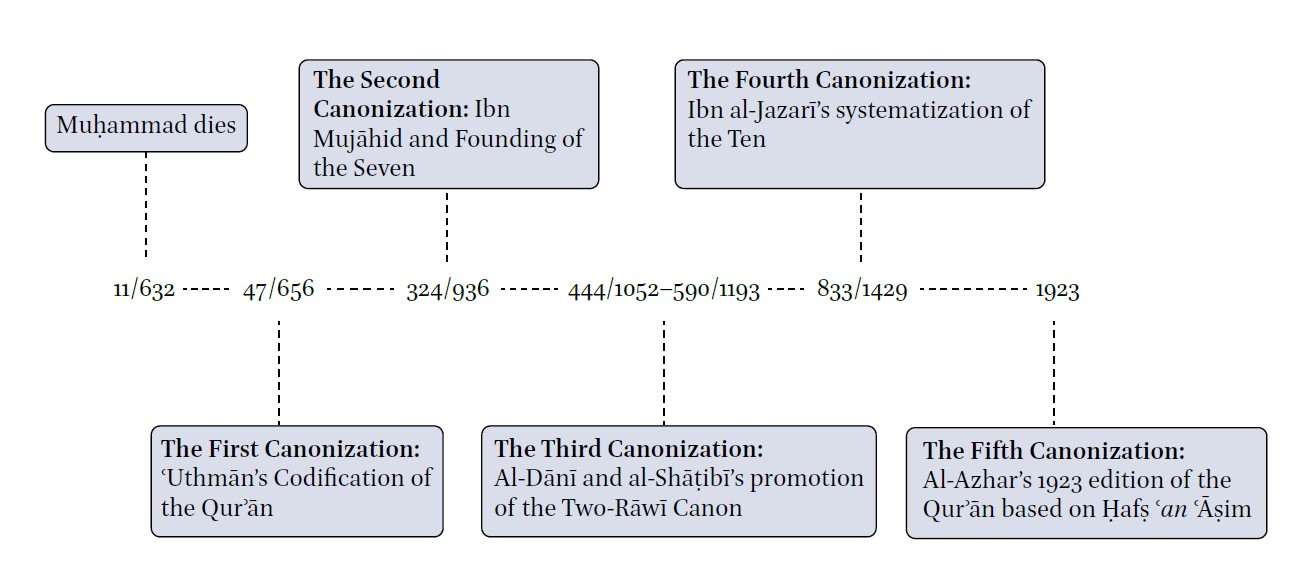
\includegraphics[width=12cm, height=4cm]{canonisation.jpg}
    %\caption{}
    \label{fig:my_label}
\end{figure}
\paragraph{}
Les variantes de la sourate éditée nous ont  montré que la notion même de variante de lecture \textit{qirāʾa} ne recouvre pas un seul sens et semble peu stable. Il y a des variantes qui peuvent  être renvoyées au \textit{rasm}  des premiers exemplaires coraniques, d'autres variantes ne sont pas forcément le résultat du \textit{rasm}, elles sont  des variantes grammaticales. Il faut aussi noter  l'absence d'une étude globale et bien fouillée sur la nature et la typologie des variantes de lecture et les modalités de vocalisation progressive du texte. Les études consultées dans  ce sens restent soit  dans le cadre descriptif  et historique restreint soit dans la disciplinarisation musulmane stricte ( hadith, grammaire, \textit{tafs\=ir} ...etc). Très peu d'études et de chercheurs  interrogent plusieurs disciplines à la fois comme l'étude de  Gregor Sholer \textit{Écrire et transmettre dans le débuts de l'islam } citée plus haut.                                                                                                                                                                                                                                                                                                                                                                                                                                                                                                                                                                                                                        \paragraph{}  
Les modalités de la transmission du savoir et des des textes  est aussi un  aspect important dans l'histoire du texte coranique et ses variantes. L'édition et l'analyse des certificats de lecture-audition \textit{samāʿ} et des licences de transmission \textit{iǧāza}  de l'un des manuscrits de cette étude  a montré une forte relation entre les  variantes de lecture et la grammaire. En effet,  au VIIème siècle,  l'intérêt pour la grammaire s'accompagne très souvent par un semblable intérêt pour les variantes de lecture comme nous avons  essayé de montrer plus haut.  

Enfin, l'étude des variantes de lecture selon  la perspective linguistique permettra de comprendre certains traits des vieux manuscrits coraniques, la relation entre l'oral et l'écrit et surtout comment s'est effectué  le passage d'un texte non vocalisé à un texte semi-vocalisé puis entièrement vocalisé. Que s'est -il passé  lors de chaque étape de  la transmission du texte.    Doit-on parler d'une simple transmission, de   transmission -dérivation ou   encore une transmission-dégradation...? 








    




\chapter*{Bibliographie générale}
\addcontentsline{toc}{chapter}{Bibliographie générale}

ََ  
   \begin{enumerate} [I]
        \item  \textbf  {Sur le Coran, traduction,  \textit{rasm} et vocalisation moderne}
        \end{enumerate}

        \begin{enumerate}
           

      
       \item   Le Coran selon la lecture de Ḥafs (version dématérialisée), KFGQPC (King Fahd Glorious Quran Printing Complex, Uthmanic Script HAFS, Version  2.0.  
       
       \url{https://qurancomplex.gov.sa}

       
       
       \item Coran 12-21  \url {https://coran12-21.org/fr}  
       \item  Masson Denise,\textit{ Le Coran, introduction, traduction et notes}, Éditions Gallimard, 1967.
       
      

     la conversion des dates a été faite  sur : \url{https://www.aly-abbara.com/utilitaires/calendrier/calendrier_hijir.html}
   \end{enumerate}  


   \begin{enumerate} [II]
        \item  \textbf  {Les catalogues des manuscrits }
        \end{enumerate}
\begin{enumerate}
\item Carl Brockelmann, \textit { Tārīḫ al-ʾdab al-ʿarabī, } (trad de l’allemand par ʿAbd al-ḥalīm al-Naǧǧār), le Caire, dār al-maʿārif, 5ème éd, ? .
    

\item  Zusgin Fuat, \textit{Tār\=iḫ al-turaṯ al-ʿarabī}, (trad de l'allemand par Maḥmūd Ḥiǧāzī), Arabie Saoudite, Ǧāmiʿat al-imām Moḥamad b. Saʿ\=ud,  1991. 

 \item  \textit{al-fahras al-šāmil li-turaṯ al-ʿarabī al-maḫṭūt}̣, muʾasasat  ͗ʾāl al-Bayt,  2ème édition, 1994.
 
\item Les catalogues ci-après sont rédigés en turc ancien \textit{osmanli}. Voici une traduction et translittération vers l'arabe.

\begin{itemize}
    \item  \textit{Fahras maktabat Fayḍ allāh ʾAfandī wa šayḫ Murād waqalqān Ismāʿīl  ʾĀġā Dultali}̄,  Dār Saʿādat [=Istanbul actuellement], 1310 [=1892]  
    
    \item \textit{ Fahras maktabat Dāmād Zādah qāḍī ʿaskar Moḥamad Murād},  Dār Saʿādat [=Istanbul actuellement], 1311 [=1893]  
\end{itemize}
    \item  Lien vers les catalogues de la bibliothèque de  Khuda Bakhsh Oriental Public Library, L'Inde.   Voir rubrique Manuscript catalogues, Qurani Science (vol.18)
  
  \url{https://kblibrary.bih.nic.in/}
    
   
\end{enumerate}
 \newpage  
\begin{enumerate} [III]
   
   \item  \textbf  {Sources primaires}
    
    \begin{enumerate}
       \normalsize

        \item al-Zubaydī abū Bakr, \textit {Ṭabaqāt al-naḥwiyīn wa al-luġawiwīn}, (éd) abu al-Faḍl Ibrāhim,  le Caire, Dār al-maʿārif , 1984.

        \item  al-Nadīm abū al-Faraǧ , \textit{Kitāb al-fihrist}, (éd) Gustav Flügel, Leipzig, Verlag Von F.C.F. Vogel, 1871. 
        
       \textemdash\textemdash  . al-Nadīm abū al-Faraǧ , \textit{Kitāb al-fihrist}, (éd) Fuʾād al-Sayyīd, Londres, Muʾsasat al-furqān  li al-turāṯ al-islāmī, 2009.

\item  al-Q\=al\=i abū  ʿAlī ,  \textit{ ki\=ab al-am\=al\=i}, (éd) Moḥamed al-Asmaʿī, le Caire,  Dār al-kutūb al-Miṣriyya, 1926. 
      \item al-Naʿīmī ʿAbd al-Qādar  , \textit{Al-dāris fī tārīḫ al-madāris}, (éd) Ibrāhīm Šams al-Dīn, Beyrouth, Dār al-kutub al-ʿilmiya, 1990. 

      \item 
 al-Fārisī abū ʿAlī, \textit{ Al-ḥuǧǧa li-lqurāʾ al-sabaʿa
 ʾa ʾimat  t  al-  ʾ amsār b- al-Ḥiǧāz wa  al- ʿIrāq wa al-Šām al-llad̠īna ḏakarahūm Abū bakr b. Muǧāhid     }, (éd) Badr al-Dīn Qahwaǧī et Bašīr Ḥwīǧbāt\=i, Damas,  Dār al-maʾmūn li-turāṯ,  1974.

 \textemdash\textemdash al-Fārisī abū ʿAlī,\textit {Kitāb al-šiʿr,} (éd) Maḥmud al-Ṭanāḥī, le Caire, maktabat al-ḫānǧi ,
 1988.

 \textemdash\textemdash  al-Fārisī abū ʿAli, \textit{Kitāb al-takmila,} (éd) Kāẓim Baḥr al-Murǧān, Beyrouth, ʿĀlam al-Kutub,  1999.

 \textemdash\textemdash  al-Fārisī abū ʿAl\=i   , \textit{  ͑Kitāb al-Īḍāḥ}, (éd) Kāẓim Baḥr al-Murǧān, Beyrouth,   ͑ Ālam al-Kutub, 1996.


\textemdash\textemdash  al-Fārisī abū ʿAl\=i \textit{
Al-masāʾil al-šširāziyat},(éd) Ḥasan Handāwī, Riyad,  kunūz išbīlyā li-našr wa tawzīʿ,  2004.
 
 \textemdash \textemdash al-Fārisī abū ʿAl\=i, \textit{al-Taʿlīqa ʿalā  kitāb sībawayh}, (éd) ʿAwaḍ al-Quzī, ? , 1990.
 
 \item  al-Ǧurǧān\=i ʿAbd al-Qāhar
   \textit {Al-muqtasad fī šarḥ al-īḍāḥ}, (éd) Kāẓm Bahr al-Murǧān, Iraq, 1982.

\item abū al-Ḥusayn b. ʿAbd allāh dit (Ibn al-Ṭarāwa) 
   \textit {Risālat al-ifṣāḥ bi-baʿḍ mā ǧāʾ min al- ḫaṭʾa fī al-īḍāḥ ,}
   (éd) Ḥātam al-ḍāman, ʿĀlam al-Kutub, 2ème éd, 1992.


 \item al-Saḫāwī ʿAlam al-dīn  ,\textit { Ǧamāl al-qurāʾ wa kamāl al-iqrāʾ},(éd) ʿAbd al-Ḥaq Sayf al-Qāḍī, Beyrouth, muʾasasat al-kutub al-ṯaqāfiya, ?.
\item Quṭrub  abū  ʿAlī, 
 \textit{Maʿānī al-qurʾān wa muškil iʿrābih} (éd) Moḥamad Laqrīz, Riyad, Dār al-Rušd, 2021.


\item al-Rūmī al-Ḥamawī Yaqūt, \textit{Muʿǧam al-ʾdabāʾ iršād al-ʾarīb ilā maʿrifat al-ʾdīd}, (éd) Iḥsān ʿAbās, Beyrouth, Dār al-ġarb al-islāmī, 1er éd, vol 1, 1993

\item al-Suyūṭī Ǧalāl al-dīn,\textit{ Al-Muzhir fī ʿulum al-luġa wa anwāʿihā}, (éd) Aḥmed Ǧād Bek et al, Beyrouth, manšurāt al-maktaba al-ʿasriyya, vol 1, 1982

 \textemdash\textemdash 
al-Suyūṭī Ǧalāl al-dīn,\textit {Buġyat al-wuʿāt fi tabaqāt al-naḥwiyīn wa al-luġawiwīn},?, maṭbaʿat ʿīsā al-bābī al-ḥalabī wa šurakaʾih, vol 1,  1964.


\item al-Baġdādī al- Ḫaṭīb\textit{, Tārih̬ madīnat al-salām},  (éd) Bašār ʿAwād, Beyrouth, Dār al-Ǧarb al-islāmī, 2001.


\item  al-Hamaḏ̠āni al-Muntaǧab,\textit{ Al-Kitāb al-Farīd fī iʿrāb  al-qurʾān al-maǧīd}, (éd) Muḥamad al-Fattayaḥ, Médine, Dār al-zamān li al-Našr wa al-Tawzīʿ, 6 Vol,  2006



\item  al-Samaʿānī ʿAbd al-Karīm, \textit{Al-ʾAnsāb,} (éd) ʿAbd al-Raḥmān al-Yamānī et al, Haydar Bād, Dāʾirat al-maʾārif al-ʿuṯmāniyya, 1er éd, 1962. 

\item abū al-Ḥassan  Saʿīd b. Masʿada   dit (al-ʾAḫfaš al-Awsaṭ), \textit{Maʿānī al-qurʾān}, (éd) Hudā Qarāʿa, maktabat al-ḫānǧī, le Caire, 1990.

\item Ibn Muǧāhid Musā, \textit{kitāb al-sabʿa}, (éd) Ḍayf Šawq\=i, Le Caire, dār al-maʿārif, 1972.


\item ʿAbd allāh b. Mālik al-Andalusī (Ibn Mālik), \textit{Matn alffiyat ibn Mālik},  (éd) ʿAbd al-Latṭīf al- Ḫaṭīb,  Kuwait, maktabat Dār al- ʿAuruba, 1er éd, 2002.


\item Ġaylān  al-ʿAdawī, \textit{The Diwān of G̲h̲ailân ibn ʿUqbah known as Dhû r-Rummah}, (éd) C.H.H .Macartney,  Cambridge, 1919. 

    
\textemdash\textemdash  Ġaylān al-ʿAdawī, \textit{Dīwān Ḏī al-Rrumma}, (éd) Ab\=u Ṣalih ʿAbd al-Qudus, Beyrouth, muʾasasat al-risāla, 1993.

\item  Ibn Mālik Anas, \textit { Al-muwaṭṭaᵓ (riwāyat yaḥya b. yaḥya al-Layṯi)}, (éd) Publications du haut conseil scientifique, 2ème éd, Vol 1,  Rabat, 2019, p.375.



\item 
Yaḥyā al-Farrāʾ\textit{,Maʿānī al-qurʾān}, (éd) ʿAlī al-Nadǧār et al,  le Caire, Dār al-Kutub al-Miṣriyya, 1955. 



    \end{enumerate} 
    
  
    
    
    
    
    
    
    

    \newpage

     \begin{enumerate} [IV]
     
    
    \item \textbf{ Sources secondaires}

    \end{enumerate}
    
    \begin{enumerate} 

    
     \item al-Munǧid Salāh al-Dīn, « Iǧāzāt al ͗samāʿ   fī al-maḫ̬ṭūṭātal-qadīma», in : \textit{maǧalat maʿhad al-maḫ̬ṭūṭāt al-͑ʿarabiyya}, le Caire, Vol 1,  1955.

\item  al-ʾUyūnī Sulaymān,\textit{ Ḥawāšī Kitāb Sibawayh}, Dār ṭayba al- ḫaḍrāʾ, Riyad, 2021.
  \item Breuil Eddie,\textit{Méthodes et pratiques de l'édition  des textes et documents modernes}, Paris, classiques garnier, 2019.
  \item ʿUḍayma ʿAbd al- Ḫāliq, \textit {Fahāris  Kitāb  Sībawayh}, ?, ?, 1985.
        
\item  Catach Nina et al, \textit{Les éditions critiques problèmes techniques et éditoriaux,} Besançon, Annales littéraires de l'université de Besançon, 1984.  
        



       \item Déroche François, \textit{Le Coran une histoire plurielle essai sur la formation du texte coranique}, Seuil, Paris, 2019.
       
\textemdash \textemdash  Déroche François, Richard, F, \textit{Scribes et manuscrits du Moyen-Orient,} Paris, Bibliothèque nationale de France, 1997.




\textemdash \textemdash     Déroche  François et al  \textit{ Manuel de codicologie des manuscrits en écriture arabe}, Paris, Bibliothèque Nationale de France, 2000.

\textemdash \textemdash Déroche François, \textit{ La voix et le calame : les chemins de la canonisation du Coran}, Paris, Collègue de France, 2016.

\item Dutton Yasin, « Orality, litteracy and ‘seven aḥruf Ḥadith », in : \textit{Journal of islamic studies}, 23.1, 2012.
\item  Fleisch Henri, \textit{Traité de philologie arabe }, vol. I ,Beyrouth, imprimerie catholique, 1961.

  \textemdash\textemdash  Fleisch Henri, \textit{Traité de  philologie arabe}, vol. II, Beyrouth, Dar El-Machreq,  2008.

\item Gacek Adam, \textit{Arabic Manuscripts A Vademecum for Readers}, Brill, Leiden, 2009.

\textemdash  \textemdash Gacek Adam, \textit{The arabic manuscript tradition, a glossary of technical terms and bibliography}, Brill, Leiden, 2001. 

\item 	Gehn Paul (dir), \textit{Lire le Manuscrit médiéval, observer et décrire},Paris,  Armand Colin (2ème éd), 2017. 

    \item Gimaret Daniel, \textit{Une lecture muʿtazilite du Coran}, Louvain-Paris, Peeters-École Pratique dès Hautes Études, 1994.
    
\item Guillaume Jean Patrick, « L'hypothèse grecque et le débat sur les origines de la tradition grammaticale arabe», in :\textit{ Histoire Épistémologie Langage}, 43-1, 2021.






\item 	Guesdon Marie-Geneviève, « La numérotation des cahiers et la foliotation dans les manuscrits arabes datés jusqu’à 1450 », in : \textit{Revue des mondes musulmans et de la Méditerranée}, 99-100, 2002.


    \item Hadj-Salah Abderrahman, \textit{Linguistique arabe et linguistique générale essai de méthodologie et d'épistémologie de 'ilm al-'arabiyya}, Alger,2 vol, Publications de l'Académie algérienne de la langue arabe, 2011.
\item 	 Hassan Chahdi, \textit{Le muṣḥaf dans les débuts de l'islam : recherches sur sa constitution et étude comparative de manuscrits coraniques anciens et de traités de qirā'āt, rasm et fawāṣil}, Thèse de doctorat inédite, sous la direction de François Déroche, Ecole pratique des hautes études, Paris, 2016. 

\textemdash \textemdash  Hassan Chahdi,  « Le paradoxe de la transmission des \textit{qiraʾāt} entre \textit{riwāya} et \textit{qiyās} ? », in :\textit{ Journal of Quranic Studies},  19-3, 2017.

        \item Humbert Geneviève, \textit{Les voies de transmission de kitāb de sībawayhi}, Leiden, Brill, 1995.
        
\item Larcher Pierre,\textit{Syntaxe de de l'arabe classique}, Aix-en-Provence, Presses Universitaires de Provence, 2017.


\item Stéfan Leder et al, \textit{Muʿǧam al- Samāʿāt al-Dimašqiyya  al-muntaḫaba 550-750h/1135-1344,} Damas, Institut français d’études arabes à Damas,1996.
\textemdash\textemdash  Leder Stéfan et al, \textit{Documents fac-similés des certificats d’audition à Damas 550-750h./1135-1344,} Damas, Institut français d’études arabes,  vol II,2000.

  
\item Lemaire Jacque, \textit{Introduction à la codicologie}, Publications de l’institut d’études médiévales de l’université catholiques de Louvain, Louvain la-Neuve, 1989.

     \item Messling Markus, \textit{Les hiérogylphes de Champollion philologie et conquête du monde}, Grenoble, Ellug, 2015.
       

    
\item Mohammed Ali Amir-Moezzi et Guillaume Dye (dir), \textit{Le Coran des historiens}, Paris, les Éditions du Cerf, 2019.

\item 	Muzerelle Denis, \textit{Vocabulaire codicologique : répertoire méthodique des termes français relatifs aux manuscrits}, Paris, Éditions CEMI, 1985.  



\item Nwīhaḍ ʿĀdal, \textit {Muʿǧam ʿulamaʾ al-Ǧazāir min ṣadr al-Islām ilā al-ʾaṣr al-ḥadī}ṯ, Beyrouth,  muʾasasat Nwīhaḍ al-ṯaqāfiya, 1er, 1980











   \item  Nasser Shady Hekmat, \textit{The transmission of the Variant Readings the problème of tawātur and the émergence of shawādhdh}, Leiden-Boston, 2013.

\textemdash \textemdash 	 Nasser Shady Hekmat, \textit{The Second Canonization
of the Qurʾān (324/936) Ibn Mujahid and the Founding of the Seven Readings}, Brill, Leiden-Boston, 2020.

	
 

 



\item Pouzet Louis, \textit{Damas au VII/ XIIIème siècle vie et structures religieuses d'une métropole islamique}, Beyrouth, D\=ar al-Machreq, 1988.

\item Qutbddin Tahera,\textit{Arabic oration art and function }, Leiden, Brill, 2019. 

  \item \normalsize   Schoeler Gregor, \textit{Écrire et transmettre dans les débuts de l'islam}, Paris, PUF, 2002.
  \item Sublet Jacqueline, \textit{Le voile du nom essai sur le nom propre arabe,} Paris, PUF, 1990.
  \item 	Theodor Nöldeke, \textit{The history of the Qurān}, edited and translated by Wolfgang H. Behn, Leiden, Brill, 2013.

\textemdash\textemdash Theodor Nöldeke,\textit {Tārīḫ al-quraʾān}, revu par Friedrich Schwally, (trad de l’allemand par Géorges Tāmer et al), Beirut, Konrad-Adenauer-Stiftung , 1er éd, 2004.
\item	Trotter David, \textit{Manuel de la philologie de l’édition}, Berlin, de Gruyter,  2015. 
  

\item  Vajda Georges, \textit{La transmission du savoir en Islam (VIIe-XVIIIe siècles)}, édité par Nicole Cottart, London, Variorum Reprints, 1983.
\item Van Putten  Marijn, \textit{Quranic Arabic
From its Hijazi Origins to its Classical Reading Traditions}, Leiden-Boston, Brill, 2022.

\item Vielliard Françoise et Guyotjeannin Olivier, \textit{Conseils pour l’édition des textes médiévaux fascicule I : conseils généraux}, Paris, École nationale des chartes, 2014.


        
        
    \end{enumerate}
\end{enumerate}

























\end{french}

\end{document}